% v2-acmsmall-sample.tex, dated March 6 2012
% This is a sample file for ACM small trim journals
%
% Compilation using 'acmsmall.cls' - version 1.3 (March 2012), Aptara Inc.
% (c) 2010 Association for Computing Machinery (ACM)
%
% Questions/Suggestions/Feedback should be addressed to => "acmtexsupport@aptaracorp.com".
% Users can also go through the FAQs available on the journal's submission webpage.
%
% Steps to compile: latex, bibtex, latex latex
%
% For tracking purposes => this is v1.3 - March 2012

\documentclass[prodmode,acmtecs]{acmsmall} % Aptara syntax

% Package to generate and customize Algorithm as per ACM style
\usepackage[ruled,linesnumbered]{algorithm2e}
\usepackage{graphicx}
\usepackage{amsmath}
\usepackage{subfigure}
\usepackage[normalem]{ulem}
\usepackage{longtable}
\usepackage{rotating}
\usepackage{threeparttable}
\usepackage{amssymb}
\usepackage{multirow}
%\usepackage{booktabs}
%\usepackage{multirow}

\renewcommand{\algorithmcfname}{ALGORITHM}
\SetAlFnt{\small}
\SetAlCapFnt{\small}
\SetAlCapNameFnt{\small}
\SetAlCapHSkip{0pt}
\IncMargin{-\parindent}

% Metadata Information
\acmVolume{9}
\acmNumber{4}
\acmArticle{39}
\acmYear{2010}
\acmMonth{3}

\newtheorem{assumption}{Assumption}
%\newtheorem{corollary}{Corollary}

% Document starts
\begin{document}

% Page heads
\markboth{X. Niu et al.}{Identifying failure-causing schemas in the presence of multiple faults}

% Title portion
\title{Identifying minimal failure-causing schemas in the presence of multiple faults}
\author{XINTAO NIU and CHANGHAI NIE
\affil{State Key Laboratory for Novel Software Technology, Nanjing University}
JEFF Y. LEI
\affil{Department of Computer Science and Engineering, The University of Texas at Arlington}
Hareton Leung and ALVIN CHAN
\affil{Department of Computing, Hong Kong Polytechnic University}
Xiaoyin Wang
\affil{Department of Computer Science, University of Texas at San Antonio}
}
% NOTE! Affiliations placed here should be for the institution where the
%       BULK of the research was done. If the author has gone to a new
%       institution, before publication, the (above) affiliation should NOT be changed.
%       The authors 'current' address may be given in the "Author's addresses:" block (below).
%       So for example, Mr. Abdelzaher, the bulk of the research was done at UIUC, and he is
%       currently affiliated with NASA.

\begin{abstract}
Combinatorial testing (CT) has been proven effective in revealing the failures caused by the interaction of factors that affect the behavior of a system. The theory of Minimal Failure-Causing Schema (MFS) has been proposed to isolate the root cause of a failure after CT. Most algorithms that aim to identify MFS focus on handling a single fault in the System Under Test (SUT). However, we argue that multiple faults are more common in practice, under which masking effects may be triggered so that some failures cannot be observed. The traditional MFS theory lacks a mechanism to handle such effects; hence, they may incorrectly isolate the MFS. To address this problem, we propose a new MFS model that takes into account multiple faults. We first formally analyse the impact of the multiple faults on existing MFS identifying algorithms, especially in situations where masking effects are triggered by multiple faults. We then develop an approach that can assist traditional algorithms to better handle multiple faults. Empirical studies were conducted using several kinds of open-source software, which showed that multiple faults with masking effects do negatively affect traditional MFS identifying approaches and that our approach can help to alleviate these effects.
%Combinatorial testing (CT) has been proven effective in revealing the failures caused by the interaction of factors that affect the behavior of a system. The theory of Minimal Failure-Causing Schema (MFS) has been proposed to isolate the root cause of a failure after CT. Most algorithms that aim to identify MFS focus on handling a single fault in the System Under Test (SUT). However, we argue that multiple faults are the more common testing scenario, under which masking effects may be triggered so that some failures cannot be observed. The traditional MFS theory, as well as the related identifying algorithms, lack a mechanism to handle such effects; hence, they may incorrectly isolate the MFS in the SUT.  To address this problem, we propose a new MFS model that takes into account multiple faults. We first formally analyse the impact of the multiple faults on existing MFS identifying algorithms, especially in situations where masking effects are triggered by multiple faults. We then develop an approach that can assist traditional algorithms to better handle multiple faults scenario. Empirical studies were conducted using several kinds of open-source software, which showed that multiple faults with masking effects do negatively affect traditional MFS identifying approaches and that our approach can help to alleviate these effects.

%Many algorithms has been proposed to find the MFS in SUT, in our recently studies, however, we find these approaches cannot behave effectively when encounter multiple faults. The main reason why these methods failed to behave normally is that most of them ignore the masking effects hiding test cases, which can bias their identified results. In this paper, we extend the MFS theory to make it support the multiple faults testing scenarios, and hence can deal masking effects. Based on this, we gave an approach to identify the MFS which can alleviate the impact of masking effects for multiple faults.

%analysed how the masking effect of multiple faults affect on the isolation of failure-inducing combinations. We further give a strategy of selecting test cases to alleviate this impact, which works by pruning these test cases that may trigger masking effect and replacing them with no-masking-effect ones. The test case selecting process repeated until we get enough information to isolate the failure-inducing combinations. We conducted some empirical studies on several open-source software. The result of the studies shows that multiple faults as well as the masking effects do exist in real software and our approach can assist combinatorial-based failure-inducing identifying methods to get a better result when handling multiple faults in SUT.
%A key problem in CT is to isolate the failure-inducing combinations of the related failure as it can facilitate the debugging efforts by reducing the scope of code that needs to be inspected. Many algorithms has been proposed to identify such combinations, however, most of these studies either just consider the condition of one failure or ignore masking effects among multiple faults which can bias their identified results.
\end{abstract}


\category{D.2.5}{Software Engineering}{Testing and debugging}[Debugging aids,testing tools]
\terms{Reliability, Verification}

\keywords{Software Testing, Combinatorial Testing, Failure-causing schemas, Masking effects}

\acmformat{Xintao Niu,
Changhai Nie,  Jeff Y. Lei,  Hareton Leung, and Alvin Chan, 2015.Identifying minimal failure-causing schemas in the presence of multiple faults.}
% At a minimum you need to supply the author names, year and a title.
% IMPORTANT:
% Full first names whenever they are known, surname last, followed by a period.
% In the case of two authors, 'and' is placed between them.
% In the case of three or more authors, the serial comma is used, that is, all author names
% except the last one but including the penultimate author's name are followed by a comma,
% and then 'and' is placed before the final author's name.
% If only first and middle initials are known, then each initial
% is followed by a period and they are separated by a space.
% The remaining information (journal title, volume, article number, date, etc.) is 'auto-generated'.

\begin{bottomstuff}
This work was supported by the National Natural Science Foundation of China (No. 61272079), the Research Fund for the Doctoral Program of Higher Education of China (No.20130091110032), the Science Fund for Creative Research Groups of the National Natural Science Foundation of China(No. 61321491), and the Major Program of National Natural Science Foundation of China (No. 91318301)
\end{bottomstuff}

\maketitle


\section{Introduction} \label{sec:introd}
With the increasing complexity and size of modern software, many factors, such as input parameters and configuration options, can affect the behaviour of the SUT. The failures caused by the interaction of these factors can make software testing challenging, especially when the interaction space is large. In the worst case, we need to examine every possible interaction of these factors as each interaction may cause unique failure \cite{song2012itree}. While exhaustive testing achieves maximal test coverage, it is impractical and uneconomical. One remedy for this problem is Combinatorial Testing (CT)\footnote{ Another term for CT is Combinatorial Interaction Testing, which is abbreviated as CIT. In this paper, they are uniformly cited as Combinatorial testing (CT).}, which systematically samples the interaction space and selects a relatively small set of test cases that cover all valid interactions, with the number of factors involved in each interaction no more than a prior fixed integer, i.e., the \emph{strength} of the interaction. Many works in CT aim to construct the smallest set of test cases \cite{cohen1997aetg,bryce2005framework,cohen2003constructing,lei2008ipog}, which is also called \emph{covering array}.

Once failures are detected by a covering array, the failure-inducing interactions in the failing test cases should be isolated. This task is important as it can facilitate debugging efforts by reducing the scope of code that is needed for inspection. \cite{ghandehari2012identifying}. However, information from a covering array sometimes is not sufficient to identify the failure-inducing interactions \cite{colbourn2008locating}. Thus, additional information is often needed. Consider the following example \cite{bach2004pairwise}, Table \ref{MS_word} presents a two-way covering array for testing an MS-Word application in which we want to examine various interactions of options for `Highlight', `Status Bar', `Bookmarks' and `Smart tags'. Assume the third test case failed. We can get six  two-way suspicious interactions that may be responsible for this failure. They are (Highlight: Off, Status Bar: On), (Highlight: Off, Bookmarks: Off), (Highlight: Off, Smart tags: Off), (Status Bar: On, Bookmarks: Off), (Status Bar: On, Smart tags: Off),  and (Bookmarks: Off, Smart tags: Off). Without additional information, it is difficult to figure out the specific interactions in this suspicious set that caused the failure. In fact, considering that the higher strength interactions could also be failure-inducing interactions, e.g., (Highlight: Off, Status Bar: On, Smart tags: Off), the problem becomes more complicated.

\begin{table}
  \tbl{MS word example\label{MS_word}}{
  \centering
  \begin{tabular}{c|cccc|c}
id& \emph{Highlight} & \emph{Status bar} & \emph{Bookmarks}& \emph{Smart tags} & \bfseries{Outcome} \\\hline
1& On & On & On& On & PASS\\ \hline
2& Off & Off & On & On & PASS\\ \hline
3&Off&	On&	Off&Off & Fail\\ \hline
4&On & Off & Off &On&  PASS\\ \hline
5&On & Off &On & Off&  PASS\\ \hline
  \end{tabular}
  }
\end{table}

To address this problem, prior work \cite{nie2011minimal} specifically studied the properties of the failure-inducing interactions in the SUT, based on which additional test cases were generated to identify them.
%the MFS theory was proposed, it propose the complete life circle of software, studied the properties of the failure-inducing combinations and the test cases, based on which, it propose the . This task, in detail, following the detecting process in the CT life-cycle\cite{nie2011minimal,nie2011survey}, needs to. The proposed MFS theory \cite{nie2011minimal} present a completed seven-step methodology to detect and isolate such failure-inducing combinations, in which this is belong to the failure diagnosis circle.
Other approaches to identify the failure-inducing interactions in the SUT include building a tree model \cite{yilmaz2006covering}, adaptively generating additional test cases according to the outcome of the last test case \cite{zhang2011characterizing}, ranking suspicious interactions based on some rules \cite{ghandehari2012identifying}, and using graphic-based deduction \cite{martinez2008algorithms}, among others.


%These approaches can be partitioned into two categories \cite{colbourn2008locating} according to how the additional test cases are generated: \emph{adaptive}--additional test cases are chosen based on the outcomes of the executed tests \cite{nie2011minimal,ghandehari2012identifying,niu2013identifying,zhang2011characterizing,shakya2012isolating,wang2010adaptive,li2012improved}or \emph{nonadaptive}--additional test cases are chosen independently and can be executed parallel \cite{yilmaz2006covering,colbourn2008locating,martinez2008algorithms,martinez2009locating,fouche2009incremental}.

Most existing approaches mainly focus on the ideal scenario in which SUT only contains one fault, under which the outcomes of test cases can be simply categorized into failure or pass. However, in this paper, we argue that SUT with multiple faults is the more common testing scenario in practice, which will result in many distinguished failures as outcomes of test cases, and moreover, this affects the effectiveness of Failure-inducing Interactions Identifying (FII) approaches. The major challenge imposed by multiple faults is dealing with the masking effect.  A masking effect \cite{dumlu2011feedback,yilmaz2013reducing} occurs when some failures prevent test cases from checking interactions that are supposed to be tested. Take the Linux command \emph{Grep} for example. We notice that there are two different failures reported in the bug tracker system. The first \footnote{http://savannah.gnu.org/bugs/?29537}  claims that Grep incorrectly matches unicode patterns with `\textbackslash$<$\textbackslash$>$', while the second \footnote{http://savannah.gnu.org/bugs/?33080} claims an incompatibility between option `-c' and `-o'. When we put these two scenarios into one test case, only one failure will be observed, which means the other failure is masked by the observed failure. This effect prevents test cases from being executed normally, leading to incorrect judgment of the correlation between the interactions checked in the test case and the failure that has been masked. This effect was firstly noted by Dumlu and Yilmaz in \cite{dumlu2011feedback}, in which they found that the masking effect in CT can prevent traditional covering array in testing some interactions.
%and they proposed a feedback-driven approach to work around them. Their recent work \cite{yilmaz2013reducing} further empirically studied the impact on the Failure-inducing Combinations Identifying(FII) approach :  Classification Tree Approach(CTA) \cite{yilmaz2006covering}, of which CTA has two versions, i.e., ternary-class and multiple-class.

%While all these approaches can help developers to isolate the failure-inducing combinations in failing test cases, in our recently studies on several open-source software, however, we found these approaches suffered from \emph{masking effects} of multiple faults in SUT. This effect was firstly introduced by Dumlu and Yilmaz in \cite{dumlu2011feedback}, in which they found that the masking effects in CT can make traditional covering array failed detecting some combinations and they proposed a feedback-driven approach to work around them. Their recent work \cite{yilmaz2013reducing} further empirically studied the impact on the Failure-inducing Combinations Identifying(FII) approach :  Classification Tree Approach(CTA)\cite{yilmaz2006covering}, of which CTA has two versions, i.e., ternary-class and multiple-class.

%Obviously this fact do trouble these algorithms as it make them unable to judge whether the test case under testing trigger only the failure observed or triggered both two failures. As a result, it will make wrong analysis in the failure-inducing interactions for these masked failures.

As masking effect can negatively affect the performance of FII approaches, a natural question is how this effect biases the results of these approaches. In this paper, we formalize the process of identifying the failure-inducing interactions under the circumstances in which masking effects exist in the SUT and try to answer this question. One insight from the formal analysis is that we cannot completely avoid the impact of masking effects even if we do exhaustive testing. Even worse, either ignoring the masking effects or treating different failures as the same failure is detrimental to the FII process.

To address this concern, we propose a strategy to alleviate this impact by adopting a divide and conquer framework. With this framework, FII approaches are scheduled to separately handle each failure in the SUT. Specifically, for a particular failure, FII approaches only focus on the test cases that either pass or trigger the same failure under analysis. Test cases that triggered other different failures will be replaced with some newly generated test cases. In this way, FII approaches can properly work with little interference from the negative masking effects.
%By this, our strategy can reduce the interference by any failure other than the failure under analysis.  trigger different failures, we will replace them with some newly regenerated test cases. These new test cases should either pass or trigger the same failure under analysis.

%we pick the test cases generated by FII approaches that trigger any failure other than the failure under analysis and

The key to our strategy is to search for a test case that does not trigger \emph{unexpected} failures, i.e., failures different from the one under analysis. To guide the search process, a natural idea is to take some characteristics from the existing test cases, and make the characteristics of the newly searched test case as disparate from the test cases which triggered unexpected failures as possible. To achieve this target, we define the \emph{suspiciousness} of a factor with respect to the failure. The higher the \emph{suspiciousness} a factor is related to a particular failure,  the greater the likelihood that the factor will trigger this fault. We then use the integer linear programming (ILP) technique to find a test case which has the least \emph{suspiciousness} with unexpected failures.

%As it is not a natural. The inution is to learn from previous test cases generating process, to avoid the similar test case. To accomplish this task, we introduce the suspicous note that record the related strength to each other failure, and then


%Our initial work demonstrated that the extent varies to what different FII approaches suffered from the masking effects, as a result, follow-on work in this paper was proposed to construct an additional voting system, in which we take comprehensive account of various result from different algorithms. We rank the suspicious MFS according to the frequency it appeared in each algorithm's output, and recommend the MFS which has a high ranking.

% For example, for the CTA, we will generate more test cases to keep as the same coverage as possible after we deleting some unsatisfied test cases from original covering array. While for the One Fact One Time approach(OFOT for short), we will repeat generating test case until we find a test case can test the fixed part as well as not trigger unsatisfied failure or until a prior ending criteria is met.

%In our recent studies on some open-source software, however, we found they didn't behave as expected when . Thorough a in-depth analysis, we learned the reason why they didn't behave as expected is that most of these approaches mainly consider the SUT just contain one failure, i.e., the oracle of the test case either be false or pass. The main reason why these methods fails to behave normally is that they didn't consider the masking effect that may happens among different failures. Obviously this fact do trouble these algorithms as it make them unable to judge whether the test case under testing trigger only the failure observed or triggered both two failures. As a result, it will make wrong analysis in the failure-inducing interactions for these masked failures.

%One remedy to alleviate this problem is to select test cases to reduce the bias, i.e., select test cases that without suffering the masking effect to get a partial but masking-avoiding result. However, most selecting strategy in CT is to cover the interactions with the number of test cases as small as possible.  So in this paper we proposed a strategy for selecting test cases with the aim to alleviate the masking effect.

%The key to the strategy is to prune test cases that may trigger a masking effect and then select or generate other test cases to test the interactions which were supposed to be tested in these pruned ones. We will keep these pruned test cases for the next iteration to isolate the failure-inducing interactions in these test cases. The process repeated until we characterize all the interactions for each failure. A point need to be noted is that these interactions supposed to be tested in the pruned test cases for one interaction vary in different algorithms we adopted. For example, for the classified tree method, we will generate more test cases that keep the same coverage, and for the one fact one time, we will generate test cases to keep the same.

To evaluate the effectiveness of our approach, we applied our strategy on the FII approach FIC\_BS \cite{zhang2011characterizing}. The subjects used were two open-source software systems found in the developers' forum in the Source-Forge community. Through studying their bug reports in the bug tracker system as well as their user manuals, we built a testing model which can reproduce the reported bugs with given test cases. We then compared the FII approach augmented with our strategy to the original FII approach. We further empirically studied the performance of the important component of our strategy -- searching for desired test cases. To conduct this study, we compared our approach with the augmented FII approach by randomly searching for desired test cases. We finally compared our approach with the only existing masking handling technique -- FDA-CIT \cite{yilmaz2013reducing}. Our studies show that our replacing strategy as well as the test case searching component achieved a better performance than the traditional approaches when the subject encountered  multiple faults, especially when these faults can induce masking effects.

%applied the traditional FII approaches and their augmented versions to identify the failure-inducing combinations in the subjects respectively. The results of our empirical studies shows that the masking effects do impact on the FII approaches, although to what the extent varies, and the approaches augmented with our strategy can identify failure-inducing combinations more accurately than traditional ones when facing masking effects, and moreover, this performance can get further improvement with using voting system.

The main contributions of this paper are:
\begin{itemize}
\item We formally analysed the relationships between failure-inducing interactions and test sets. (Section \ref{sec:formal})
\item We provide an theoretical framework for explaining how traditional FII approaches work. (Section \ref{subsec:Formal:identi})
\item We studied the impact of the masking effects caused by multiple faults on FII approaches. (Section \ref{sec:mask})
\item We proposed an efficient test case replacement strategy to alleviate the impact of these effects (Section \ref{sec:method}), and gave an MFS identification approach augmented with this replacement strategy (Section \ref{sec:appraoch}).
%\item We proposed a divide and conquer strategy for selecting test cases to alleviate the impact of these effects.
%\item We designed an efficient test case searching method which can find a test case that does not trigger an unexpected failure.
\item We conducted several empirical studies and showed that our strategy can assist FII approaches to achieve better performance in identifying failure-inducing interactions in the SUT with masking effects. (Section \ref{sec:emprical})
\end{itemize}


%In our recent studies, however, we find these algorithms cannot behave as expected in some subject software. Through a deep analysis, we find that there are multiple faults with different levels in these subject. It means that when we set up a test configuration and execute the SUT to observe the result, the high level failure will trigger first and perturb we examining the code that may trigger the low level failure. As a result we will omit some options or component in this test configuration that may be the cause of the low level failure. We call this a masking effect which make the MFS identifying algorithms not able to work properly.

%In this paper, we propose a approach that can assist these algorithms to avoid these masking effect. Our framework consists of three parts: first, it will use the statistic analysis technique--dominate tree to analysis the test script and then collect the information traditional identifying algorithms. of code lines in this script. Second, we will support a interface called "Record" for the MFS identifying algorithms that each time the algorithm encounter a failure should call this interface. So that we can record this failure as well as the code lines that trigger this failure. Last, this framework support these algorithms the interface "analysis" that can tell them whether the failure they encounter having masked some failure else.

%First we will comprehensively analysis this two programs to get the MFSs and their corresponding failure level as the basic information for the left experiment.
%To evaluate the effectiveness of our framework, we took two widely-used open source software as our experiment subject. And then we will choose five MFSs identifying  algorithms, for each algorithm, we will compare the identifying result among two versions of this algorithm, one using our framework while another one not. The result of the empirical studies shows that our framework can assist the MFS identifying algorithm in getting a more accurate result.


%The rest of this paper is organised as follows:
%section 2 gives a simple example to motivate our work. Section 3 give some background of the work. Section 4 describe our approach in detail. Section 5 illustrate the experiment and reports the result. Section 6 discusses the related works. Section 7 provides some concluding remarks.

\section{Motivating example} \label{sec:motiv}
\begin{figure}
\begin{verbatim}
public float foo(int a, int b, int c, int d){
  //step 1 will cause an exception when b == c
  float x = (float)a / (b - c);

  //step 2 will cause an exception when c < d
  float y = Math.sqrt(c - d);

  return x+y;
  }
\end{verbatim}
\caption{A simple program \emph{foo} with four input parameters}
\label{toy-program}
\end{figure}
We use a small example to motivate our approach. Assume a method \emph{foo} has four input parameters: \emph{a, b, c, } and \emph{d}. The four parameter types are all integers and their values are: $v_{a} = \{7, 11\}, v_{b} = \{2, 4, 5\}, v_{c} = \{4, 6\}, v_{d} = \{3, 5\}$. The code of \emph{foo} is shown in Figure \ref{toy-program}.

There are two potential failures of \emph{foo}: first, in step 1 we can get an \emph{Arithmetic Exception} when $b$ is equal to $c$, i.e.,  $b = 4$ and $c = 4$, that causes a division by zero. Second, another \emph{Arithmetic Exception} will be triggered in step 2 when $c < d$, i.e., $c = 4$ and $d = 5$, taking square root of a negative number. So the expected failure-inducing interactions in this example should be (-, 4, 4, -) and (-, -, 4, 5).

FII approaches do not consider the code detail; instead, they apply black-box testing, i.e., feed inputs to the programs and execute them to observe the result. The basic proposition of FII approaches is that the failure-inducing interactions for a particular failure can only appear in those test cases that trigger this fault. FII approaches often aim at using as few test cases as possible to get the same (or approximate) result as exhaustive testing, so the results derived from an exhaustive testing set are the best that FII approaches can achieve. Here, we will show how exhaustive testing works to identify the failure-inducing interactions for the program.

\begin{table}[ht]
  \tbl{Test cases and their corresponding result\label{test-example}}{
  \centering
  \begin{tabular}{ccc}
id&test case & result\\\hline
1&(7, 2, 4, 3) &  PASS\\ \hline
2&(7, 2, 4, 5) &  Ex 2\\ \hline
3&(7, 2, 6, 3) &  PASS\\ \hline
4&(7, 2, 6, 5) &  PASS\\ \hline
5&(7, 4, 4, 3) &  Ex 1\\ \hline
\textbf{6}&\textbf{(7, 4, 4, 5)} &  \textbf{Ex 1}\\ \hline
7&(7, 4, 6, 3) &  PASS\\ \hline
8&(7, 4, 6, 5) &  PASS\\ \hline
9&(7, 5, 4, 3) &  PASS\\ \hline
10&(7, 5, 4, 5) &  Ex 2\\ \hline
11&(7, 5, 6, 3) &  PASS\\ \hline
12&(7, 5, 6, 5) &  PASS\\ \hline
  \end{tabular}
  \hspace{1em}
  \begin{tabular}{ccc}
id&test case & result\\\hline
13&(11, 2, 4, 3)& PASS\\ \hline
14&(11, 2, 4, 5)& Ex 2\\ \hline
15&(11, 2, 6, 3)& PASS\\ \hline
16&(11, 2, 6, 5)& PASS\\ \hline
17&(11, 4, 4, 3)& Ex 1\\ \hline
\textbf{18}&\textbf{(11, 4, 4, 5)}& \textbf{Ex 1}\\ \hline
19&(11, 4, 6, 3)& PASS\\ \hline
20&(11, 4, 6, 5)& PASS\\ \hline
21&(11, 5, 4, 3)& PASS\\ \hline
22&(11, 5, 4, 5)& Ex 2\\ \hline
23&(11, 5, 6, 3)& PASS\\ \hline
24&(11, 5, 6, 5)& PASS\\ \hline
  \end{tabular}
  }
  \end{table}

We first generate every possible test case listed in the column ``test case" of Table \ref{test-example}. The execution results are listed in the result column of Table \ref{test-example}. In this column, \emph{PASS} means that the program runs without any exception. \emph{Ex 1} indicates that the program triggered an exception corresponding to step 1 and \emph{Ex 2} indicates the program triggered an exception corresponding to step 2. From the data listed in Table \ref{test-example}, we can determine that (-, 4, 4, -) must be the failure-inducing interaction of Ex 1 as all the test cases that triggered Ex 1 contain this interaction. Similarly, interactions (-, 2, 4, 5) and  (-, 5, 4, 5) must be the failure-inducing interactions of Ex 2. We list these interactions and the corresponding exceptions in Table \ref{identify-example}.

\begin{table}[ht]
\centering
 \tbl{Identified failure-inducing interactions and their corresponding Exception\label{identify-example}}{
\begin{tabular}{c c}
Failure-inducing interaction & Exception\\ \hline
(-, 4, 4, -) &  Ex 1\\ \hline
(-, 2, 4, 5) &  Ex 2\\ \hline
(-, 5, 4, 5) &  Ex 2\\ \hline
\end{tabular}
}
\end{table}

Note that in this example we did not get the expected result with traditional FII approaches. The failure-inducing interactions for Ex 2 are (-,2,4,5) and (-,5,4,5),  respectively, instead of the expected interaction (-,-,4,5). So why did we fail to get the (-,-,4,5)? The reason lies in \emph{test case  6} (7,4,4,5) and \emph{test case 18} (11,4,4,5). These two test cases contain the interaction (-,-,4,5), but they did not trigger Ex 2; instead,  Ex 1 was triggered.

% if more than two failures, and the masking element is more, the result we got will be more noisy so that we cannot figure out the reals result

Now consider the source code of \emph{foo}. If Ex 1 is triggered, it will stop executing the remaining code and report the exception result. In other words, Ex 1 may mask Ex 2. Let us re-examine the interaction (-,-,4,5). If we suppose that \emph{test case 6} and \emph{test case 18} should trigger Ex 2 if they did not trigger Ex 1, then we can conclude that (-,-,4,5) should be the failure-inducing interaction of Ex 2, which is identical to the expected one. However, we cannot get this result, unless we fix the code that triggers Ex 1 and re-execute all the test cases.

% we cannot validate the supposition that \emph{test case 6} and \emph{test case 18} should trigger Ex 2 when they did not trigger Ex 1.

 So in practice, \emph{when we lack resources to execute all the test cases repeatedly or can only do black-box testing, a more economical and efficient approach to alleviate the masking effect on FII approaches is desired}.

\section{Formal model of Minimal Failure-causing schema} \label{sec:formal}
This section presents some definitions and propositions for a formal description of failure-inducing interactions and test sets.

\subsection{Minimal Failure-causing Schemas} \label{sec:introd:mfs}

Assume that the behaviour of a SUT is influenced by \emph{k} parameters, and each parameter $p_{i}$ has $a_{i}$ discrete values from the finite set $V_{i}$, i.e., $a_{i}$ = $|V_{i}|$ ($i$ = 1,2,...,\emph{k}). In practice, these parameters can represent many factors, such as input variables, run-time options, building options, etc. Next we will give some formal definitions,  Definitions \ref{de:test}, \ref{de:tuple}, \ref{de:sub} were originally defined in \cite{nie2011survey}.

%\newdef{definition}{Definition}
\begin{definition}\label{de:test}
A \emph{test case} of a SUT is a set of \emph{k} values, one for each parameter of the SUT, which is denoted as a \emph{k}-tuple ($v_{1}$, $v_{2}$,...,$v_{k}$), where $v_{1}\in V_{1}$, $v_{2} \in V_{2}$ ... $v_{k} \in V_{k}$.
\end{definition}

For the example in Section \ref{sec:motiv}, ($a = 7$, $b = 2$, $c = 4$, $d = 3$) is a test case, which is actually a group of values being assigned to each input parameter.
%We need to execute the SUT with these test cases to ensure the correctness of its behaviour.

\begin{definition}
A \emph{failure} is an abnormal execution of a test case.
\end{definition}
In CT, such a \emph{failure} can be a thrown exception, compilation error, assertion failure or constraint violation. In this paper, failures are classified according to the the specific \emph{fault} information. For example, if failures have the same exception traces information, they are treated as the same failure. The main point in this paper is to study the impact of multiple different \emph{failures} on failure-inducing interactions identification.

To facilitate our discussion, we introduce the following assumptions that will be used throughout this paper:

\begin{assumption}
The execution result of a test case is deterministic.
\end{assumption}
This assumption is a common assumption of CT fault diagnosis\cite{wang2010adaptive,zhang2011characterizing,ghandehari2012identifying,li2012improved,niu2013identifying}. It indicates that the outcome of executing a test case is reproducible and will not be affected by some random events.
\begin{assumption}
Different failures in the SUT can be distinguished by various information such as exception traces, state conditions, or the like.
\end{assumption}
This assumption indicates that the testers can detect different failures during testing. As different failures will complicate fault diagnosis tasks, distinguishing them is the first step to resolve them.

\begin{assumption}
All the tests are valid in the SUT, i.e., there is no \emph{inter-option} constraints in the SUT.
\end{assumption}
Here \emph{option} indicates the parameter of a SUT. This assumption shows that we can always determine the outcome after executing a test case, i.e., either pass or fail with some exceptions.

In practice, these assumptions may not be satisfied. In Section \ref{sec:assumptions}, we will discuss their impact on the theories and approach proposed in this paper, as well as the measures to alleviate them. Particularly for the third assumption, we will show that one type of inter-option constraint is essentially equal to a specific failure. Thus we can directly use the approach in this paper to solve it.


%In practice, these two assumptions will not always be satisfied. Elimination of them can introduce the probabilistic and clustering parts into our model, which will further complicate our analysis and so we will not discuss them in this paper.
Now let us consider the condition that some failures are triggered by some test cases. It is then desirable to determine the cause of these failures and hence some parameter values of the failing test cases must be analysed.
%\end{definition}

%Figuring out the test case as well as the executing result is usually not enough to analyse the source of the bug, especially when there are too many parameters we need to care in this test case. In this circumstance, we need to study some subsets of this test case, so we need the following definition:

%Figuring out the execution outcomes of test cases must reveal the presence of faulty interactions among those considered. However, the location and magnitude of the fault is still far from clear, especially when there are too many parameters we need to care in this test case. Hence, we need to study some subsets of this test case, which can help isolate the cause of failures.

\begin{definition} \label{de:tuple}
For the SUT, the $\tau$-tuple (-,$v_{b_{1}}$,...,$v_{b_{\tau}}$,...) is called a $\tau$-degree \emph{schema} ($0 < \tau \leq k $) when some $\tau$ parameters have fixed values and the others can take on their respective allowable values, represented as ``-".

When $\tau = k$, $\tau$-degree \emph{schema} is actually a test case. Furthermore, if every fixed value in a schema is in a test case, we say this test case \emph{contains} the schema.
%, which can be denoted as $k-degree\  combination \in T$
\end{definition}

For example,  (-, 4, 4, -) in  Table \ref{identify-example} is a $2$-degree schema. And the test case (7, 4, 4, 3) contains this schema.

\begin{definition} \label{de:sub}
Let $c_{1}$ be a \emph{m}-degree schema, $c_{2}$ be an \emph{n}-degree schema in the SUT, and $m < n$. If all the fixed parameter values in $c_{1}$ are also in $c_{2}$, then $c_{2}$ \emph{subsumes} $c_{1}$. In this case, we can also say that $c_{1}$ is a \emph{sub-schema} of $c_{2}$, and $c_{2}$ is a \emph{super-schema} of $c_{1}$, denoted as $c_{1} \prec  c_{2}$.
\end{definition}

For example, in the motivating example, the $2$-degree schema (-, 4, 4, -) is a sub-schema of the $3$-degree schema (-, 4, 4, 5), that is, (-,4,4,-) $\prec$ (-,4,4,5).

According to definition 3.4, it is obvious that the subsuming relationship `$\prec$' is transitive, i.e., if $c_{1} \prec c_{2}, c_{2} \prec c_{3}$, then $c_{1} \prec c_{3}$.
%Note that as a test case $t$ can be deemed as a $k$-degree schema, if it contains a schema $c$, then it can be regarded as $c \prec t$.

\begin{definition} \label{de:mfs}
If for any test case, as long as it contains the schema $c$, it will trigger the failure of particular fault $F$. Then we call $c$ the \emph{failure-causing schema} of $F$. Additionally, if none of the sub-schema of $c$ is the \emph{failure-causing schema} of $F$, we then call $c$ the \emph{Minimal Failure-causing Schema} (MFS) of $F$.
%Based on this, if a test case $t$ contain such a failure-inducing combination, say $c(F)$, it should trigger the failure $F$, for which the test case can be put as $t(F)$
\end{definition}

In fact, MFS is identical to the failure-inducing interactions discussed previously. Identifying MFS helps to focus on the root cause of a failure and thus facilitates the debugging efforts. Note that all the failures discussed in this paper are option-related \cite{yilmaz2006covering}. That is, all the failures are caused by the interactions of the parameter values in the SUT. Another noteworthy point is that, in practice, we may not accurately obtain the MFS according to the MFS definition (Section 3.5). This is because in some specific cases,  e.g., the masking problems which we will discussed later, we may not determine whether some test cases will trigger the failure of particular failure of $F$, or not.

%We have the following proposition based on these basic definitions.
%
Some notations used later are listed below for ease of reference:
\begin{itemize}
\item $k$ : The number of parameters that influence the SUT.
\item $V_{i}$ : The set of discrete values that the $i$th parameter of the SUT can take.
\item $T^{*}$ :  The exhaustive set of test cases for the SUT. For a SUT with $k$ parameters, and each parameter can take $|V_{i}|$ values, the number of test cases in $T^{*}$ is $\prod_{i = 1}^{k} |V_{i}|$. Note that some test cases may be invalid if there exists constraints among the parameters.
\item $T$ : A set of test cases. (Similarly for $T_{i},\ T_{j}, ...$. )
\item $\bar{T}$ : The complementary test set of T, i.e., $\bar{T} \bigcup T = T^{*},\ \bar{T} \bigcap T = \varnothing$.
\item $A \backslash B$ :  The set of elements that belong to set $A$ but not to $B$. For example $T_{i} \backslash T_{j}$ indicates the set of test cases that belong to set $T_{i}$, but not to $T_{j}$.
\item $L$ : The number of faults contained in the SUT.
\item $F_{m}$ : The $m$th fault in the SUT ($1 \leq m \leq L$);  A failure which is classified to \emph{fault} $F_{m}$ is called \emph{failure} of $F_{m}$.
\item $T_{F_{m}}$ :  All the test cases that can trigger the failure of $F_{m}$ in the SUT.
\item $\mathcal{T}(c)$ :  All the test cases that contain the schema $c$ in the SUT. Based on the definition of MFS, we know that if schema $c$ is an MFS of $F_{m}$, then $\mathcal{T}(c) \subseteq T_{F_{m}}$. Note that, there may be multiple MFS for $F_{m}$
%\item $T_{mask(F_{m})}$ :  All the test cases that contain the
%\item $T_{mask(F_{m})}$ :
%\item $T_{mask(F_{m})}$ :

\item $\mathcal{I}(t)$ :  All the schemas that are contained in the test case $t$, e.g., $\mathcal{I}(\ (1 1 1)\ )= \{(1 - -)(- 1 -)(- - 1)(1 1 -)(1 - 1)(- 1 1) (1 1 1)\} $.
\item $\mathcal{I}(T)$ :  All the schemas that are contained in test set $T$, i.e., $\mathcal{I}(T) = \bigcup_{t\in T} \mathcal{I}(t)$.
\item  $\mathcal{S}(T)$:  All the schemas that are only contained in test set $T$ (Referred to as \emph{Special schemas}); $\mathcal{S}(T) =  \mathcal{I}(T) \backslash \mathcal{I}(\bar{T}) $.
\item  $\mathcal{C}(T)$ : A set of the minimal schemas that are only contained in test set $T$ (Referred to as \emph{Minimal schemas}); $\mathcal{C}(T) =  \{c | c \in \mathcal{S}(T)\ and\ \not\exists c' \prec c, s.t., c' \in \mathcal{S}(T)\}$.

\end{itemize}

%Let $c_{m}$ be a m-degree schema, we denote the set of all the test cases can \emph{contain} the schema $c_{m}$ as $T(c_{m})$. Further, for the test case $t$, let $\mathcal{I}(t)$ to denote the set of all the schemas that are contain by $t$, and for the set of test cases $T$, we let $\mathcal{I}(T) = \bigcup_{t\in T} \mathcal{I}(t)$. Then we have the following propositions.


%\newtheorem{proposition}{Proposition}


%\emph{first important proposition :  every is the subset!}

\subsection{Relations between schemas and test sets} \label{sec:introd:proposition}

\begin{proposition}[{smaller schema $c$ has a larger $\mathcal{T}(c)$}] \label{pro:shl}
For schemas $c_{1}$, $c_{2}$, if $c_{1} \prec c_{2}$, then all the test cases that contain $c_{2}$ must also contain $c_{1}$, i.e., $\mathcal{T}(c_{2}) \subseteq \mathcal{T}(c_{1})$.
\end{proposition}

%\begin{proof}
%  $ \forall t \in \mathcal{T}(c_{2})$,  $t$ contains $c_{2}$. As $t$ is a $k$-degree schema, then it has $c_{2} \prec t$ .  As $c_{1} \prec c_{2}$, then $c_{1} \prec t$, indicating that $t$ contains $c_{1}$. Therefore, $t \in \mathcal{T}(c_{1})$. So it follows that $\mathcal{T}(c_{2}) \subseteq \mathcal{T}(c_{1})$.
%\end{proof}

We omit the proof of this proposition as it is quite obvious. Suppose a SUT with four binary parameters, which can be denoted as SUT($2^4$). Table \ref{example_subsume} illustrates an example of the Proposition \ref{pro:shl}. The left column lists the schema $c_{2}$ = (0,0,-,-) as well as all the test cases in $\mathcal{T}(c_{2})$, while the right column lists the schema $c_{1}$ = (0,-,-,-) and $\mathcal{T}(c_{1})$. We can see that when $c_{1} \prec c_{2}$, $\mathcal{T}(c_{2}) \subseteq \mathcal{T}(c_{1})$.

\begin{table}[ht]
\centering
\tbl{Example of Proposition \ref{pro:shl}\label{example_subsume}}{
  \begin{tabular}{c}
$c_{2}$ \\ \hline
(0, 0, -, -) \\ \hline
 $\mathcal{T}(c_{2})$\\ \hline
(\textbf{0}, \textbf{0}, 0, 0)\\
(\textbf{0}, \textbf{0}, 0, 1)\\
(\textbf{0}, \textbf{0}, 1, 0)\\
(\textbf{0}, \textbf{0}, 1, 1)\\  \hline
  \end{tabular}
  \hspace{3em}
  \begin{tabular}{c}
$c_{1}$ \\ \hline
(0, -, -, -) \\ \hline
 $\mathcal{T}(c_{1})$\\ \hline
(\textbf{0}, 0, 0, 0)\\
(\textbf{0}, 0, 0, 1)\\
(\textbf{0}, 0, 1, 0)\\
(\textbf{0}, 0, 1, 1)\\
(\textbf{0}, 1, 0, 0)\\
(\textbf{0}, 1, 0, 1)\\
(\textbf{0}, 1, 1, 0)\\
(\textbf{0}, 1, 1, 1)\\  \hline
  \end{tabular}
  }
  \end{table}

\begin{proposition}[Property of special schema set of test set T]\label{pro:stct}
For any test set $T$ of the SUT,  $\bigcup_{c \in \mathcal{S}(T)}\mathcal{T}(c) = T$.
\end{proposition}
\begin{proof}
As $\mathcal{S}(T) =  \mathcal{I}(T) \backslash \mathcal{I}(\bar{T}) $,  $\forall c \in \mathcal{S}(T),\ c \in \mathcal{I}(T)\ and\ c \not\in \mathcal{I}(\bar{T})$. Then $\forall t \in \mathcal{T}(c), t \ contains\ c$, indicating that $t \in T$.  Hence, $\mathcal{T}(c) \subseteq T$.  Then $\bigcup_{c \in \mathcal{S}(T)}\mathcal{T}(c) \subseteq T$.

On the other hand, $\forall t \in T$,  $\exists c' \in \mathcal{I}(t)$, such that $c' \not\in \mathcal{I}(\bar{T})$ (at least it holds when $c' = t$). Hence, $c' \in \mathcal{S}(T)$.  Obviously $t \in \mathcal{T}(c') \subseteq \bigcup_{c \in \mathcal{S}(T)} \mathcal{T}(c)$. Therefore,  $ T \subseteq \bigcup_{c \in \mathcal{S}(T)}\mathcal{T}(c)$.
\end{proof}



\begin{proposition}[Property of minimal schema set of test Set T]\label{pro:ash}
For any test set $T$ of the SUT, $\bigcup_{c \in \mathcal{C}(T)} \mathcal{T}(c) = T$.
\end{proposition}

\begin{proof}
As $\mathcal{C}(T) = \{c | c \in \mathcal{S}(T)\ and\ \not\exists c' \prec c, s.t., c' \in \mathcal{S}(T)\}$, indicating that $\mathcal{C}(T) \subseteq \mathcal{S}(T)$.  It is then obviously $\bigcup_{c \in \mathcal{C}(T)} \mathcal{T}(c) \subseteq \bigcup_{c \in \mathcal{S}(T)} \mathcal{T}(c)$. Hence, we just need to prove that $\bigcup_{c \in \mathcal{S}(T)} \mathcal{T}(c) \subseteq \bigcup_{c \in \mathcal{C}(T)} \mathcal{T}(c)$.

$\forall t \in \bigcup_{c \in \mathcal{S}(T)} \mathcal{T}(c) $, $\exists c \in \mathcal{S}(T),\ s.t., t \in \mathcal{T}(c)$. According to the definition of $\mathcal{C}(T)$, $\exists c' \in \mathcal{C}(T), s.t.,\ c' = c \ or\ c' \prec c$. Correspondingly $\mathcal{T}(c') = \mathcal{T}(c),\ or\ \mathcal{T}(c) \subseteq \mathcal{T}(c')$ by Proposition \ref{pro:shl}. Hence, $t \in \mathcal{T}(c') \subseteq \bigcup_{c \in \mathcal{C}(T)} \mathcal{T}(c)$.

Therefore, $\bigcup_{c \in \mathcal{C}(T)} \mathcal{T}(c) = \bigcup_{c \in \mathcal{S}(T)} \mathcal{T}(c) = T$.
\end{proof}

Table \ref{example_minimal_schemas} gives an example of $T^{*}$, $T$, $\bar{T}$, $\mathcal{S}(T)$ and $\mathcal{C}(T)$ in SUT($2^3$). We can find that all the schemas in $\mathcal{S}(T)$ and $\mathcal{C}(T)$ are only contained in test set $T$, and for any $t \in T$, it contains at least one schema in $\mathcal{S}(T)$ and $\mathcal{C}(T)$. Additionally, $\mathcal{C}(T)$ is a minimal schema set which filters those super schemas in $\mathcal{S}(T)$.

%Further, the schemas in $\mathcal{S}(T)$ are either the super schemas of schemas in $\mathcal{C}(T)$, e.g. ((0,0,0) \prec (0,0,-)), or
% see that for any other schema not in $\mathcal{C}(T)$, either we can find a test case not in $T$ that contains the schema, e.g.,(0,0,-) with the test case (0,0,1,1) not in $T$, or that is the super schema of one of the two minimal schemas, e.g.,(0,0,0,0) is the super schema of both (0,0,0,-) and (0,0,-,0).
\begin{table}[ht]
\centering
\tbl{Example of the special and minimal schemas\label{example_minimal_schemas}}{
  \begin{tabular}{c c c  c  c }
$T^{*}$ & $T$ &$\bar{T}$ & $\mathcal{S}(T)$ & $\mathcal{C}(T)$\\ \hline
(0, 0, 0) & (0, 0, 0) &           & (0, 0, -) & (0, 0, -)\\
(0, 0, 1) & (0, 0, 1) &           & (0, -, 0) & (0, -, 0)\\
(0, 1, 0) & (0, 1, 0) &           & (0, 0, 0) & \\
(0, 1, 1) &           & (0, 1, 1) & (0, 0, 1) &\\
(1, 0, 0) &           & (1, 0, 0) & (0, 1, 0) &\\
(1, 0, 1) &           & (1, 0, 1) &           &\\
(1, 1, 0) &           & (1, 1, 0) &           &\\
(1, 1, 1) &           & (1, 1, 1) &           &\\
\hline  \end{tabular}
  }
  \end{table}

Let $T_{F_{m}}$ denote the set of all the test cases triggering the failure of $F_{m}$, then $\mathcal{C}(T_{F_{m}})$ actually is the MFS set of $F_{m}$.

%And obviously $\forall c_{m}$ we have $\mathcal{C}(\mathcal{T}(c_{m})) = \{c_{m}\}$.

According to the definition of $\mathcal{C}(T)$, one observation is  $\mathcal{C}(T) \subseteq \mathcal{S}(T)$, and for any schema in $\mathcal{S}(T)$, it either belongs to $\mathcal{C}(T)$, or is the super schema of one element of $\mathcal{C}(T)$, i.e., $\forall c \in \mathcal{S}(T), \exists c' \in \mathcal{C}(T), s.t., c' = c,\ or\ c' \prec c$.
% Another obvious observation is that
%Then, we have the following proposition.
\begin{proposition} [Minimal schema of the subset of test set $T$]\label{pro:sbS}
 For any test set $T$ and schema $c$ of the  SUT, if $\mathcal{T}(c) \subseteq T$, then  $c \in \mathcal{S}(T) $.
\end{proposition}
\begin{proof}
 Assume $c \not\in \mathcal{S}(T)$, i.e., $c \not\in \mathcal{I}(T) \backslash \mathcal{I}(\bar{T})$, then $c \in \mathcal{I}(\bar{T})$. It indicates that $\exists t \in \bar{T}, t \in \mathcal{T}(c)$, which contradicts that $\mathcal{T}(c) \subseteq T$. Therefore, $c \in \mathcal{S}(T)$.
\end{proof}

Table \ref{example_subset_minimal_schemas} shows an example of this proposition for SUT($2^3$).  In this table, the test set $\mathcal{T}(c)$ of schema $c$ is the subset of test set $T$. As a result, the special schema set $\mathcal{S}(T)$ of $T$ contains this schema $c$ = (0, 0, -).

\begin{table}[ht]
\centering
\tbl{Example of a minimal schema of the subset of a test set\label{example_subset_minimal_schemas}}{
  \begin{tabular}{c c c  c }
$c$       & $\mathcal{T}(c)$ &$T$         & $\mathcal{S}(T)$ \\ \hline
(0, 0, -) & (0, 0, 0)        & (0, 0, 0)  & (0, -, -)    \\
          & (0, 0, 1)        & (0, 0, 1)  & (0, -, 0)    \\
          &                  & (0, 1, 0)  & (0, -, 1)    \\
          &                  & (0, 1, 1)  & (0, 0, -)    \\
          &                  &            & (0, 1, -)    \\
          &                  &            & (0, 0, 0)    \\
          &                  &            & (0, 0, 1)    \\
          &                  &            & (0, 1, 0)    \\
          &                  &            & (0, 1, 1)    \\
\hline  \end{tabular}
  }
  \end{table}

Based on Proposition \ref{pro:sbS}, as long as $\mathcal{T}(c) \subseteq T$ for any schema $c$ and any test set $T$ in the SUT, $c$ either belongs to $C(T)$ or is the super-schema of some schema in $C(T)$.  Considering a more general scenario, i.e., two test sets $T_{1}$,  $T_{2}$  with $T_{2} \subseteq T_{1}$, we then can easily obtain the relationship between $\mathcal{C}(T_{1})$ and $\mathcal{C}(T_{2})$ according to Proposition \ref{pro:sbS}.


\begin{proposition}[{minimal schemas in the smaller test set}]\label{pro:ssp}
For $T_{1}$ and $T_{2}$ of the SUT with $T_{2} \subseteq T_{1}$, $\forall c_{2} \in \mathcal{C}(T_{2})$, $\exists c_{1} \in \mathcal{C}(T_{1}), s.t.,\ either\ c_{1} = c_{2} \ or\  c_{1} \prec c_{2}.$
\end{proposition}

\begin{proof}
$\forall c_{2} \in \mathcal{C}(T_{2})$,  $\mathcal{T}(c_{2}) \subseteq T_{2} \subseteq T_{1}$. According to Proposition \ref{pro:sbS}, $c_{2} \in \mathcal{S}(T_{1})$. By definitions of $\mathcal{S}(T)$ and $\mathcal{C}(T)$, $\exists c_{1} \in \mathcal{C}(T_{1}), s.t., c_{1} = c_{2},\ or\ c_{1} \prec c_{2}$.
\end{proof}

% So this proposition holds as the schema in $\mathcal{S}(T_{2})$ either is in $\mathcal{C}(T_{1})$, or must be the super-schemas of some schemas in $\mathcal{C}(T_{1})$

%Likewise, we can get the properties of the schemas identified for the larger test set.

\begin{proposition}[{minimal schemas in the larger test set}]\label{pro:sls}
For $T_{1}$ and $T_{2}$ of the SUT, $T_{2} \subseteq T_{1}$. Then $\forall c_{1} \in \mathcal{C}(T_{1})\ $, $\exists c_{2} \in  \mathcal{C}(T_{2}), s.t., \ (1)\ c_{1} = c_{2} $, $or\ (2)\ c_{1} \prec c_{2}\ $, $ or \ (3)\ \not\exists c_{2} \in \mathcal{C}(T_{2}), s.t., c_{2} \prec c_{1}\ or\ c_{2} = c_{1},\ or\ c_{1} \prec c_{2}.$
\end{proposition}

\begin{proof}
Assume that $\exists c_{1} \in \mathcal{C}(T_{1})$,  s.t., $\exists c_{2} \in \mathcal{C}(T_{2}), c_{2} \prec c_{1}$. According to Proposition \ref{pro:ssp}, as $T_{2} \subseteq T_{1}$, so $\forall c_{2} \in \mathcal{C}(T_{2})$, $\exists c_{1}' \in \mathcal{C}(T_{1}), s.t.,\ either\ c_{1}' = c_{2} \ or\  c_{1}' \prec c_{2}$. Combining them, we can get that $c_{1}' \prec c_{1}$. This is a obvious contradiction, as $c_{1}$ and $c_{1}'$ are both minimal schemas in  $\mathcal{C}(T_{1})$.

Hence, apart from the impossible relationship $c_{2} \prec c_{1}$, then $\forall c_{1} \in \mathcal{C}(T_{1})\ $, $\exists c_{2} \in  \mathcal{C}(T_{2}), s.t., \ (1)\ c_{1} = c_{2} $, $or\ (2)\ c_{1} \prec c_{2}\ $, $ or \ (3)\ \not\exists c_{2} \in \mathcal{C}(T_{2}), s.t., c_{2} \prec c_{1}\ or\ c_{2} = c_{1},\ or\ c_{1} \prec c_{2}.$
\end{proof}

We need to note the third case, i.e., $\ \not\exists c_{2} \in \mathcal{C}(T_{2}), s.t., c_{1} \prec c_{2}\ or\ c_{1} = c_{2},\ or\ c_{2} \prec c_{1}.$ We refer to this case as $c_{1}$ is \emph{irrelevant} to $\mathcal{C}(T_{2})$. Furthermore, we can also say a schema is \emph{irrelevant} to another schema if these two schemas are neither identical nor subsuming each other.

We illustrate these scenarios with examples in Table \ref{example_three_condition} for SUT($2^{3}$). There are two parts in this table, with each part showing two test sets: $T_{1}$ and $T_{2}$, which have $T_{2} \subseteq T_{1}$. In the left part, the schemas in $\mathcal{C}(T_{2})$: (0, 0, -) and (0, -, 0), both are the super-schemas of the one in $\mathcal{C}(T_{1})$:(0,-,-). While in the right part, the schemas in $\mathcal{C}(T_{2})$: (0, 0, -) and (0, -, 0) are both in $\mathcal{C}(T_{1})$. Furthermore, one schema in $\mathcal{C}(T_{1})$: (1,1,-) is irrelevant to $\mathcal{C}(T_{2})$.

\begin{table}[ht]
\centering
\tbl{Minimal schemas of two subsuming test sets\label{example_three_condition}}{
  \begin{tabular}{cc}
$T_{2}$&$T_{1}$ \\ \hline
(0, 0, 0)&(0, 0, 0)\\
(0, 0, 1)&(0, 0, 1) \\
(0, 1, 0)&(0, 1, 0)\\
         &(0, 1, 1) \\ \hline
 $\mathcal{C}(T_{2})$& $\mathcal{C}(T_{1})$ \\ \hline
(0, 0, -)&(0, -, -)\\
(0, -, 0)&		   \\ \hline
  \end{tabular}
  \hspace{1em}
  \begin{tabular}{cc}
$T_{2}$&$T_{1}$\\ \hline
(0, 0, 0) & (0, 0, 0)\\
(0, 0, 1) & (0, 0, 1)\\
(0, 1, 0) & (0, 1, 0)\\
		  & (1, 1, 0)\\
		  & (1, 1, 1)\\ \hline
$\mathcal{C}(T_{2})$& $\mathcal{C}(T_{1})$ \\ \hline
(0, 0, -)&  (0, 0, -)\\
(0, -, 0)&  (0, -, 0)\\
		 &  (1, 1, -)\\  \hline
  \end{tabular}
  }
  \end{table}

In summary, these propositions provide the foundation of MFS identification (Propositions \ref{pro:stct} and \ref{pro:ash}), and more importantly, they clarify the relationships between the minimal schemas of two different test sets (Propositions \ref{pro:sls} and \ref{pro:ssp}). As will be shown in Section \ref{sec:mask}, under the masking effects, the actual failing test set is either to be the super-set or sub-set of the observed failing test set. Hence, Propositions \ref{pro:sls} and \ref{pro:ssp} will describe the impact of masking effects on MFS identification later.
%For any test sets in the SUT, it has a set of minimal schemas.
%(b) For two subsuming test sets, their minimal schemas can be subsuming or irrelevant to each other.


\section{MFS identification}\label{subsec:Formal:identi}
In this section, we will study how traditional MFS identification approaches, i.e., FII approaches, identify the MFS. Let $T_{F}$ indicate all the failing test cases and $T_{P}$ all the passing test cases ( Note that $T_{F} \bigcap T_{P} = \varnothing$ and $T_{F} \bigcup T_{P} = T^{*}$ ). Then the MFS for the SUT is $\mathcal{C}(T_{F})$. Theoretically,  to figure out all the MFS in the SUT, we need to exhaustively execute each possible test case, and collect the failing test cases $T_{F}$. This is impossible in practice, especially when the testing space is very large.

As it is impractical to get all the MFS, an appropriate strategy is to determine some MFS of them. With the following proposition, we can learn that with the existing subset of test cases, we can also identify some of them.

\begin{proposition}[{Same minimal schemas in different test sets}]\label{pro:dsms}
For $T_{1}$ and $T_{2}$, $T_{1} \subset T_{2}$. If $\exists c \in \mathcal{C}(T_{1})$, such that $ c \in \mathcal{C}(T_{2})$. Then, for any test set $T_{3}$, such that $T_{1} \subset T_{3} \subset T_{2}$, we have $c \in \mathcal{C}(T_{3})$.
\end{proposition}

\begin{proof}
According to Proposition \ref{pro:sls}, $\forall c \in \mathcal{C}(T_{1})$, there exists $c' \in \mathcal{C}(T_{3})$, such that either $c' \prec c$ or $c' = c$. Let us assume that $c' \prec c$. As there exists $c'' \in \mathcal{C}(T_{2})$, such that $c = c''$, then $c' \prec c''$. This is contradiction as $T_{3} \subset T_{2}$. Hence, the assumption  $c' \prec c$ does not hold, indicating that $c' = c$.
\end{proof}

For example, Table \ref{example_identical_condition} shows the minimal schemas for $T_{1}$, $T_{2}$, $T_{3}$ and $T_{3}'$, where $T_{1} \subset T_{3} \subset T_{2}$ and $T_{1} \subset T_{3}' \subset T_{2}$. We can find that $\mathcal{C}(T_{1})$, i.e., (0, 0, -) is identical to that one in $\mathcal{C}(T_{2})$, which also in $\mathcal{C}(T_{3})$ and $\mathcal{C}(T_{3}')$.

\begin{table}[ht]
\centering
\tbl{Identical minimal schemas of subsuming test sets\label{example_identical_condition}}{
\begin{tabular}{lll|lll|lll|lll}
\multicolumn{3}{c|}{$T_{1}$}    & \multicolumn{3}{c|}{$T_{2}$}    & \multicolumn{3}{c|}{$T_{3}$}    & \multicolumn{3}{c}{$T_{3}'$}   \\ \hline
0       & 0       & 0      & 0       & 0       & 0      & 0       & 0       & 0      & 0       & 0       & 0     \\
0       & 0       & 1      & 0       & 0       & 1      & 0       & 0       & 1      & 0       & 0       & 1     \\
        &         &        & 1       & 1       & 1      & 1       & 1       & 1      & 1       & 1       & 0     \\
        &         &        & 1       & 1       & 0      &         &         &        &         &         &       \\ \hline
\multicolumn{3}{c|}{$\mathcal{C}(T_{1})$} & \multicolumn{3}{c|}{$\mathcal{C}(T_{2})$} & \multicolumn{3}{c|}{$\mathcal{C}(T_{3})$} & \multicolumn{3}{c}{$\mathcal{C}(T_{3})$'} \\ \hline
0       & 0       & -      & 0       & 0       & -      & 0       & 0       & -      & 0       & 0       & -     \\
        &         &        & 1       & 1       & -      & 1       & 1       & 1      & 1       & 1       & 0     \\ \hline
\end{tabular}
  }
  \end{table}

Based on Proposition \ref{pro:dsms}, let $T_{F-known}$ be the given test cases which are known to be failing, and $T_{P-known}$ be the known passing test cases. $T_{unknown} = T^{*} \setminus (T_{F-known} \bigcup T_{P-known})$ be the test cases that are not known to be failing or not, we have the following lemma:

\begin{lemma}[{Determine some MFS}]\label{pro:dsmfs}
$\forall c \in \mathcal{C}(T_{F-known})$, if $\exists c' \in \mathcal{C}(T_{F-known} $ $\bigcup T_{unknown})$, such that $c = c'$, then $c$ must be MFS.
\end{lemma}

The proof of this lemma is obvious. This is because whatever the outcomes of the test cases  $T_{unknown}$ will be, the actual failing test cases (denoted as $T_{F-acutal}$), must have $T_{F-known} \subset T_{F-acutal} \subset (T_{F-known}\bigcup T_{unknown})$. Based on Proposition \ref{pro:dsms}, this lemma holds.  With this lemma, we can determine some MFS in the SUT without executing all the test cases. However, to identify an MFS $c$, there still needs many test cases to be executed; at least, we should execute all the test cases in $ \mathcal{T}(c)$. For example, for SUT($2^{8}$), to identify the MFS (1, 1, -, -, -, -, -, -), we should make sure all the test cases contain this schema must fail, of which the number is $|T_{F-known}|$ = $2^{8-2} = 64$. This number grows exponentially with the number of parameters in the SUT. Hence, traditional FII approaches will make some assumptions to further reduce the number of needed test cases to identify the MFS.

Generally, with proper assumptions, apart from the test cases which have been executed, we can infer some of the remaining test cases to be passing or failing. Formally, let $T_{F-infer}$ refer to the test cases that can be inferred to be failing and $T_{P-infer}$ the inferred passing test cases. With the test cases whose outcomes can be inferred, the test cases which are known to failing is increased to be $T_{F-known} \bigcup T_{F-infer}$, and the unknown test cases decreased to be $T_{unknown} \setminus (T_{F-infer} \bigcup T_{P-infer})$.  Based on Lemma \ref{pro:dsmfs}, $\forall c \in \mathcal{C}(T_{F-known} \bigcup T_{F-infer})$, if it is identical to some schema in $\mathcal{C}((T_{F-known} \bigcup T_{F-infer}) \bigcup (T_{unknown} \setminus (T_{F-infer} \bigcup T_{P-infer})))$, then $c$ must be MFS.

The assumptions and corresponding inferring process vary with different FII approaches. To specifically describe the inferring processes of different FII approaches is beyond this paper. Next, we will only focus on describing the FIC\_BS appraoch\cite{zhang2011characterizing}--an efficient adaptive MFS identification approach.

%\begin{lemma}[{Determine some MFS}]\label{pro:dsmfs}
%$\forall c \in \mathcal{C}(T_{F-known})$, if it is identical to some schema in $\mathcal{C}(T_{F-known} \bigcup T_{unknown})$, then $c$ must be MFS.
%\end{lemma}

% Then the MFS identified by FII approaches can be depicted as: MFS = $\mathcal{C}(T_{f-obs} \bigcup T_{f-infer})$.
%
%Hence, Traditional approach may
%Traditional FII approaches select a subset of the exhaustive test cases to execute. Hence, we can only observe the outcomes of a part of the whole test cases. In this case, in order to identify the MFS, each of the remaining test cases (that are not observed) must be predicted to be failing or not.

%
%The algorithm of FIC\_BS is listed in the appendix, as well as the corresponding interpretation.
We will give a simple example to illustrate how FIC\_BS works. For SUT($2^{4}$), assume the test case (1, 1, 1, 1) failed, then the FIC\_BS approach can be illustrated in Table \ref{fic-bs-identify}. In this table, to identify the MFS in $t_{0}$, FIC\_BS generated 4 more test cases, i.e., $t_{1}, t_{2}, t_{3}$ and $t_{4}$. Each of these test cases consists of two parts: the same part as in the original failing test case, called the \emph{fixed} part against $t_{0}$; and the part with values different from the original failing one, called the \emph{mutated} part against $t_{0}$. For example, for test case $t_{1}$, the \emph{fixed} part (against $t_{0}$) is (-, -, 1, 1) and the \emph{mutated} part is (0, 0, -, -). Note that these mutated parts do not necessarily have to be value (0, 0, -, -). We just need make them different from what are in $t_{0}$ (This is important to the approach we later propose in the paper).  The MFS obtained by FIC\_BS is (-, 1, -, 1). This conclusion is based on the following \emph{safe value} assumption.


%These test cases are generated to reduce the discrepancy between passing test cases and failing test cases as much as possible, and finally the only one difference between a failing test case and passing test case is determined to be failure-inducing (This process is inspired by delta debugging \cite{zeller2002simplifying}, which also focus on simplifying the differences between passing and failing test cases). For example, comparing test cases $t_{1}$ and $t_{2}$ in Table \ref{fic-bs-identify}, the only difference between them is the second factor (in bold), hence (-, 1, -, -) must be one parameter value of the MFS. Similarly,  by comparing $t_{3}$ and $t_{4}$, we can learn that (-, -, -, 1) must be another parameter value of the MFS. As $t_{4}$ fails, there is no more failure-inducing parameter values; otherwise, (0, 1, 0, 1) should pass as it only contains two failure-inducing parameter values (This conclusion is based on the assumption that (0, -, -, -),(-, 0, -, -) ,(-, -, 0, -) and (-, -, -, 0)  are \emph{safe values}, i.e., none of them is the part of any MFS). Hence, the MFS of $t_{0}$ is (-, 1, -, 1).

%The pass of $t_{1}$ indicates that this test case breaks the MFS in the original test case \emph{t}. So, (1,-,-) should be one failure-causing factor, and as the other test cases ($t_{2}, t_{3}$) all failed , this means no other failure-inducing factors were broken (note that this conclusion is based on the assumption that $t$ only contains one MFS); therefore, the MFS in \emph{t} is (1,-,-).

\begin{table}[ht]
\tbl{FIC\_BS running example\label{fic-bs-identify}}{
\begin{tabular}{llllll}
\hline
\textbf{ID} & \multicolumn{4}{l}{\textbf{Test Case}} & \textbf{outcome} \\ \hline
$t_{0}$ & 1     & 1     & 1     & 1     & fail    \\ \hline
$t_{1}$ & 0     & 0     & 1     & 1     & pass    \\
$t_{2}$ & 0     & 1     & 1     & 1     & fail    \\
$t_{3}$ & 0     & 1     & 0     & 0     & pass    \\
$t_{4}$ & 0     & 1     & 0     & 1     & fail    \\ \hline
\end{tabular}}
\end{table}


%The mutated part of each additional test cases consists of safe
%
%values, i.e., none of the parameter value in mutate part is the part of any MFS.

\begin{assumption} \label{ass:safevalue}
Each parameter value of the mutated part of each additional test cases is \emph{safe value}, i.e., a value that is not the part of any MFS.
\end{assumption}

Hence, this assumption indicates that the mutated part of each additional test cases are all safe values. Based on this assumption, we have the following two corollaries:

\begin{corollary}\label{lemma:inferpassing}
 $\forall t \in T_{unknown}$, if $\exists t' \in T_{P-known}$, such that $t$ is obtained by mutating some parameter values of $t'$, and the mutated part are all safe values, then $t$ must be a passing test case.
\end{corollary}

\begin{proof}
Assume that $t$ is a failing test case. As $\{\ t\ \} \subset T_{F}$, $\exists c \in \mathcal{C}(T_{F})$, such that $c \prec t $ or  $c = t$ (Based on Proposition \ref{pro:sbS}). In other words, $\forall e \in c$, it has $e \in t$.  As $c$ has no parameter value that is safe value (c is an MFS), so $\forall e \in c$, it has $e \in (t \setminus mutate)$, where $mutate$ indicates the mutated part of $t$ against $t'$. However, as $t'$ also contain $(t \setminus mutate)$, so $t'$ should be a failing test case, which is contradiction. Hence, $t$ must be a passing test case.
\end{proof}

For example, if (0, 0, 0, 0) is known to be a passing test case, and (-, -, -, 1) \footnote{Here we use the 1-degree schema (-, -, $v_{i_{j}}$, -, -) to denote the value \emph{j} of the \emph{i}th parameter of the SUT.}  is safe value, then test case (0, 0, 0, 1) must be a passing test case.

\begin{corollary} \label{lemma:inferfailing}
$\forall t \in T_{unknown}$, if $\exists t' \in T_{F_known}$, such that $t$ is obtained by mutating some parameter values of $t'$, and the mutated part are all safe values, then $t$ must be a failing test case.
\end{corollary}

This corollary can be proved according to Corollary \ref{lemma:inferpassing}. As an example, assume (0, 0, 0, 0) is known to be a failing test case, and (-, -, -, 0) is safe value, then test case (0, 0, 0, 1) must be a failing test case.

Based on these two corollaries, we can easily infer that some unknown test cases to be failing or not. In table \ref{fic-bs-identify}, FIC\_BS assumes that (0, -, -, -),(-, 0, -, -) ,(-, -, 0, -) and (-, -, -, 0)  are \emph{safe values}. Then those inferred test cases are listed in Table \ref{realMFS-for-11} with column `State' of \emph{infer}. For example, the mutated part of $t_{2}$ against the known passing test case $t_{4}$ is the (-, -, 0, -), which is safe value, so $t_{2}$ should be inferred to be passing;  the mutated part of the known failing test case $t_{16}$ against the unknown test case $t_{14}$ is still the safe value (-, -, 0, -), so $t_{14}$ should be inferred to be failing.

\begin{table}[ht]
\tbl{Test outcomes for MFS(- 1 - 1)\label{realMFS-for-11}}{
\begin{tabular}{l|llll|l|l}
\hline
ID  & \multicolumn{4}{l|}{Test Case} & Outcome  & State  \\ \hline
$\textbf{t}_{\textbf{1}}$  &\textbf{0}      & \textbf{0}     & \textbf{0}     & \textbf{0}     & \textbf{pass} & \textbf{infer} \\
$\textbf{t}_{\textbf{2}}$  & \textbf{0}      & \textbf{0}     & \textbf{0}     & \textbf{1}     & \textbf{pass} & \textbf{infer}\\
$\textbf{t}_{\textbf{3}}$  & \textbf{0}      & \textbf{0}     & \textbf{1}     & \textbf{0}     & \textbf{pass} & \textbf{infer}\\
$t_{4}$  & 0      & 0     & 1     & 1     & pass   & known    \\
$t_{5}$  & 0      & 1     & 0     & 0     & pass    & known   \\
$t_{6}$  & 0      & 1     & 0     & 1     & fail    & known   \\
$t_{7}$  & 0      & 1     & 1     & 0     & - & unkonwn\\
$t_{8}$  & 0      & 1     & 1     & 1     & fail   & known    \\
$t_{9}$  & 1      & 0     & 0     & 0     & - & unkonwn\\
$t_{10}$ & 1      & 0     & 0     & 1     & - & unkonwn\\
$t_{11}$ & 1      & 0     & 1     & 0     & - & unkonwn\\
$t_{12}$ & 1      & 0     & 1     & 1     & - & unkonwn\\
$t_{13}$ & 1      & 1     & 0     & 0     & - & unkonwn\\
$\textbf{t}_{\textbf{14}}$ & \textbf{1}      & \textbf{1}     & \textbf{0}     & \textbf{1}     & \textbf{fail} & \textbf{infer}\\
$t_{15}$ & 1      & 1     & 1     & 0     & - & unkonwn\\
$t_{16}$ & 1      & 1     & 1     & 1     & fail  & known     \\ \hline
\end{tabular}}
\end{table}

After inferring these test cases, we can find that $\mathcal{C}(T_{F-known} \bigcup T_{F-infer})$ = $\mathcal{C}(\{t_{6}, t_{8}, t_{14}, t_{16}\})$ = (-, 1, -, 1), and $\mathcal{C}((T_{F-known} \bigcup T_{F-infer}) \bigcup (T_{unknown} \setminus (T_{F-infer} \bigcup T_{P-infer})))$ = $\mathcal{C}(\{t_{6}, t_{8}, t_{14}, t_{16}, t_{7}, t_{9}, t_{10}, t_{11}, t_{12}, t_{13}, t_{13}, t_{15}\})$ = (1, -, -, -), (-, 1, 1, -), (-, 1, -, 1). Hence, we can derive that (-, 1, -, 1) must be MFS.

%In our model, to identify MFS (-, 1, -, 1), we should execute all the test cases, and test cases in $\mathcal{T}((1, -, 1, -))$ should fail.  As listed in Table \ref{realMFS-for-11}, apart from the observed test cases in Table \ref{ofot-identify} (in bold), the outcomes of other test cases should be inferred. These results can be inferred based on the basic assumptions of FIC\_BS. For example, test case $t_{3}$ should pass, as if not so, (-, -, -, 0) must be failure-inducing factor (comparing $t_{3}$ and $t_{4}$), which contradicts the factor (-, -, -, 0) are safe value. Similarly, $t_{2}$ (Comparing $t_{2}$ and $t_{4}$), $t_{1}$ (Comparing $t_{1}$ and $t_{5}$) should pass. Additionally, $t_{14}$ should fail, because if not so, (0, -, -, -) must be failure-inducing (Comparing $t_{6}$ and $t_{14}$).


%Note that the process of FIC\_BS approach is consistent with the MFS identification model we built before. In the example listed in Table \ref{fic-bs-identify}, all the observed passing test cases, i.e., $T_{p-obs}$, is \{ $t_{1}$, $t_{3}$ \}, and all the observed failing test cases, i.e.,  $T_{f-obs}$, is  \{ $t_{0}$, $t_{2}$, $t_{4}$ \}.


This example illustrates that the FII approach does not execute all the test cases, but with proper assumptions, the schemas identified by FII can be approximate to or even the same as the exactly correct MFS in the SUT. Other FII approaches can also be built into our formal model for MFS identification, but this is beyond the scope of this paper. Even though each FII approach tries to identify the MFS as accurately as possible, masking effects will negatively affect the observed outcomes and the inferred results. We next discuss the masking problem.

\section{Masking effect} \label{sec:mask}
As discussed before, $\mathcal{C}(T_{F_{m}})$ is considered to be the MFS set of fault $F_{m}$ in theory.  When accounting for the masking effects between multiple faults, however, this consideration is not correct.

\begin{definition}
A \emph{masking effect} occurs when a test case \emph{t} contains an MFS of a particular fault, but it does not trigger the failure of expected fault because other unexpected event, such as the failure of other fault or unaccounted control dependency, was triggered earlier that prevents $t$ from being normally checked.
\end{definition}

Taking the masking effects into account, when identifying the MFS of a specific fault $F_{m}$, we must not ignore those test cases which did not trigger $F_{m}$ but should have triggered it. We call these test cases $T_{mask(F_{m})}$. Hence, the MFS of fault $F_{m}$ should be revised as $\mathcal{C}(T_{F_{m}} \bigcup T_{mask(F_{m})})$.


Going back to the motivating example in Section \ref{sec:motiv}, as \emph{test case 6} and \emph{test case 18} should trigger Ex 2 in case they did not trigger Ex 1, $T_{mask(F_{2})}$ is \{ (7,4,4,5),(11,4,4,5)\}. Hence, the MFS of $Ex 2$ is $\mathcal{C}(T_{F_{2}} \bigcup T_{mask(F_{2})})$, which is (-,-,4,5) instead of the incorrect schema set $\{(-,2,4,5), (-,5,4,5)\}$.

In practice with masking effects, however, it is not possible to correctly identifying the MFS, unless we fix some bugs in the SUT and re-execute some test cases to figure out $T_{mask(F_{m})}$.

For traditional FII approaches, without the knowledge of  $T_{mask(F_{m})}$,  two common strategies can be adopted to deal with the multiple faults problem, i.e., \emph{regarded as same failure}  and \emph{distinguishing failures}.  The former strategy treats all types of faults as one fault, and hence all the failures are considered the same, while the latter distinguishes the failures but with no special consideration of the masking effects, i.e., if a test case fails with a particular type of fault, this strategy presumes it does not contain other types of faults.
%We will separately discuss the two strategies under exhaustive testing condition and normal FII testing condition.
%\subsection{Masking effects under exhaustive testing}

\subsection{Regarded as same failure strategy} \label{sec:mask:ro}
%, as it does not distinguish the failures, i.e., it treats all types of failures as one fault--\emph{failure}, and others as \emph{pass}.
This is the most common strategy. With this strategy, the minimal schemas are the set $\mathcal{C}(\bigcup_{i = 1}^{L}T_{F_{i}})$, where $L$ is the number of all the faults in the SUT. Obviously, $T_{F_{m}} \bigcup T_{mask(F_{m})} \subseteq \bigcup_{i = 1}^{L}T_{F_{i}}$ .  By Proposition \ref{pro:sls}, some schemas obtained by this strategy may be the sub-schemas of some of the actual MFS, or be irrelevant to the actual MFS.

As an example, consider the test cases in Table \ref{masking-effects-exhaustive}. Assume we need to characterize the MFS of \emph{fault 1}. All the test cases that triggered \emph{fault 1} are listed in column \emph{$T_{F_{1}}$}; similarly, we list the test cases that triggered failures of other faults in column \emph{$T_{mask(F_{1})}$} and \emph{$T_{non\_mask(F_{1})}$}, respectively, in which the former masked \emph{fault 1}, while the latter did not. Actually the MFS of \emph{fault 1}  should be (1,1,-,-) and (-,1,1,1) as listed in the column `actual MFS of \emph{fault 1}'. However, when we use the \emph{regarded as same failure} strategy, the minimal schemas obtained will be (-,-,0,0), (1,1,-,-), (-,-,1,1), in which (-,-,0,0) is irrelevant to the actual MFS of \emph{fault 1}, and (-,-,1,1) is a sub-schema of the actual MFS (-,1,1,1).

\begin{table}[ht]
\centering
\tbl{Masking effects for exhaustive testing \label{masking-effects-exhaustive}}{
  \begin{tabular}{ccc}
$T_{F_{1}}$&$T_{mask(F_{1})}$ &$T_{non\_mask(F_{1})}$\\ \hline
(1, 1, 1, 1)& (1, 1, 0, 0) & (0, 1, 0, 0) \\
(1, 1, 1, 0)& (0, 1, 1, 1) & (0, 0, 0, 0)\\
(1, 1, 0, 1)&              & (1, 0, 0, 0)\\
          	&              & (1, 0, 1, 1)\\
        	&              & (0, 0, 1, 1)\\ \hline
actual MFS of \emph{Fault 1}&  regarded as same failure & distinguishing failures  \\
$\mathcal{C}(T_{F_{1}} \bigcup T_{mask(F_{1})})$& $\mathcal{C}( T_{F_{1}} \bigcup T_{mask(F_{1})}  \bigcup T_{non\_mask(F_{1})})$ & $\mathcal{C}(T_{F_{1}})$  \\ \hline
(1, 1, -, -)&  (-, -, 0, 0) & (1, 1, -, 1)\\
(-, 1, 1, 1)&  (1, 1, -, -) & (1, 1, 1, -)   \\
            &  (-, -, 1, 1) &         \\ \hline
  \end{tabular}
  }
  \end{table}

\subsection{Distinguishing failures strategy} \label{sec:mask:df}
Distinguishing the failures by the exception traces or error code can help identify the MFS related to a particular failure. Yilmaz \cite{yilmaz2013reducing} proposed the \emph{multiple-class} failure characterizing method instead of the \emph{ternary-class} approach to make the characterizing process more accurate. Besides, other approaches can also be easily extended using this strategy for testing the SUT with multiple faults.
%We call this strategy \emph{distinguishing failures}.

This strategy focuses on identifying the set of $\mathcal{C}(T_{F_{m}})$. As $T_{F_{m}} \bigcup T_{mask(F_{m})} \supseteq T_{F_{m}} $, by Proposition \ref{pro:ssp}, some schemas obtained by this strategy may be the super-schema of some actual MFS. Moreover, some actual MFS may be irrelevant to the schemas obtained by this strategy according to Proposition \ref{pro:sls}, which means that this strategy will \emph{ignore} these actual MFS.

For the simple example shown in Table \ref{masking-effects-exhaustive}, when using this strategy, we will get the minimal schemas (1, 1, -, 1) and (1, 1, 1, -), which are both super schemas of the actual MFS (1,1,-,-). Furthermore, no schemas obtained by this strategy have any relationship with the actual MFS (-,1,1,1), which means it was ignored.

It is noted that the motivating example in section \ref{sec:motiv} actually adopted this strategy. As a result, the schemas identified for Ex 2: (-,2,4,5), (-,3,4,5) are the super-schemas of the correct MFS(-,-,4,5).


\subsection{Masking effects for FII approaches} \label{sec:mask:fci}
Based on previous analysis, even though exhaustive testing is conducted to obtain $T_{F_{m}}$, we cannot determine the MFS set because of the masking effects. For traditional MFS identification approaches, i.e., FII approaches, masking effects can make problems worse. This is because these approaches, with masking effects, are not only unable to determine $T_{mask(F_{m})}$ as discussed before, but also unable to correctly infer the outcomes of some unexecuted test cases, i.e., wrong $T_{F-infer}$ and $T_{P-infer}$ as mentioned in Section \ref{subsec:Formal:identi}.

%This is because due to the time and computing rescouses limitation, FII approaches can only execute part of the whole test cases. Consequently, only part of $T_{F_{m}}$ can be observed. Under this condition, the remaining of $T_{F_{m}}$ need to be inferred. The inference process, which is based on the executed test cases and their outcomes, is key to the quality of the MFS identification result.


Consider a FII example that still use the FIC\_BS method \cite{zhang2011characterizing}.  Similar to the example listed in Table \ref{fic-bs-identify}, assume the test case (1, 1, 1, 1) failed with $F_{1}$ (The MFS is still assumed to be (-, 1, -, 1) as Table \ref{fic-bs-identify}). Then assume that there exists an MFS (-, 1, 0, -) that triggers $F_{2}$, where fault $F_{2}$ can mask $F_{1}$. Next we will illustrate how FIC\_BS works using  strategies the \emph{regarded as same failure} strategy and \emph{distinguishing failures} strategy, respectively.

First, for the \emph{regarded as same failure} strategy, we list how it works in Fig. \ref{fig:maskingeffects1}, as well as the masking effects it suffers. With this strategy, it just needs three additional test cases to determine the MFS in the original failing test case $t$, i.e., $t_{1}'$, $t_{2}'$, and $t_{3}'$ (listed in the left part of Fig. \ref{fig:maskingeffects1}).
 The right part of Fig. \ref{fig:maskingeffects1} shows the MFS it obtained is (-, 1, -, -), which is obviously wrong (See the correct result in Table \ref{realMFS-for-11}, which should be (-, 1, -, 1), but this strategy treats its sub-schema (-, 1, -, -) to be MFS). The middle part of Fig. \ref{fig:maskingeffects1} explains why this strategy obtained this result. Specifically, it treats all failures as the same failure, i.e., failure of $F_{1}$. Hence, test case $t_{5}$ in the middle of Fig. \ref{fig:maskingeffects1} (Marked \emph{Strategy} in the column `State ') is determined to trigger $F_{1}$. Here, the test case $t_{5}$ corresponds to the test case $t_{3}'$ in the left part of Fig.\ref{fig:maskingeffects1}.  According to the corollaries \ref{lemma:inferpassing} and \ref{lemma:inferfailing}, test cases $t_{1}$, $t_{2}$, $t_{3}$, $t_{6}$, $t_{7}$, $t_{13}$, $t_{14}$, and $t_{15}$ are determined to be pass or fail with $F_{1}$, respectively. Afterward, we can determine that (-, 1, -, -) should be the MFS. This is because, $\mathcal{C}(T_{F_{1}})$ = $\mathcal{C}(\{t_{5}, t_{6}, t_{7}, t_{8}, t_{13}, t_{14}, t_{15}, t_{16} \})$ = (-, 1, -, -), which has been included in $\mathcal{C}(T_{F_{1}} \bigcup T_{unknown}$ = $\mathcal{C}(\{t_{5}, t_{6}, t_{7}, t_{8}, t_{9}, t_{10}, t_{11}, t_{12}, t_{13}, t_{14}, t_{15}, t_{16}\})$ = (1, -, -, -), (-, 1, -, -).


\begin{figure}[htbp]
\centering
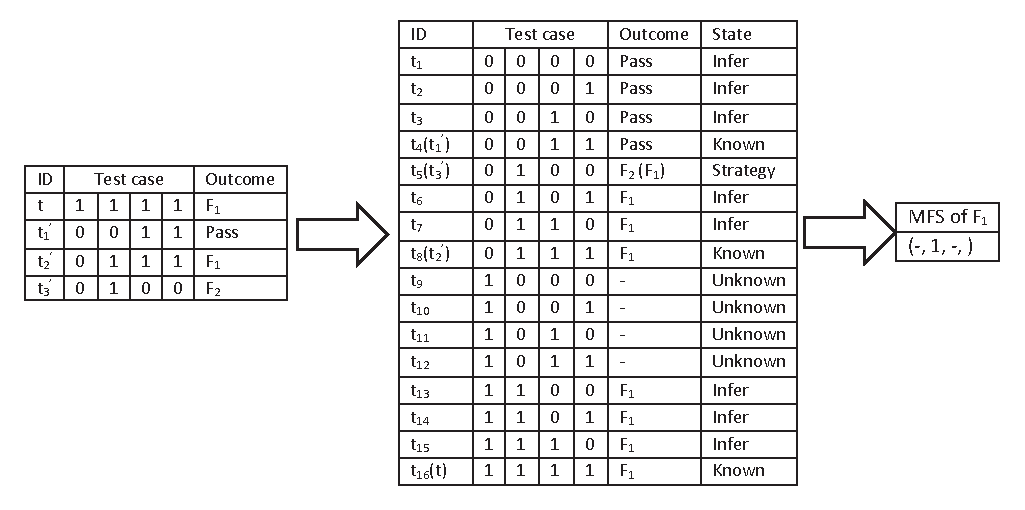
\includegraphics[width=4.99in]{example-of-masking-effects1.eps}
\caption{Masking effects of strategy Regarded as same failure}
\label{fig:maskingeffects1}
\end{figure}

For the second strategy, i.e., \emph{distinguishing failures}, we list the result in Fig. \ref{fig:maskingeffects2}. Different from the first strategy, it treats the different failures other than $F_{1}$ as pass. As a result, test cases $t_{5}$ and $t_{6}$ in the middle part of Fig. \ref{fig:maskingeffects2} are determined to be pass.  Then combining the inferred test cases, it finally gets the MFS (-, 1, 1, 1), which is also not correct (This schema is the super-schema of the original MFS of $F_{1}$ (-, 1, -, 1)).

%only $t_{3}$ breaks the MFS. In this case, the MFS is considered to be (-, -, 1, -), which is the sub-schema of the original one.  While for the second strategy, i.e., \emph{distinguishing failures}, it determines $t_{1}$ and $t_{2}$ as \emph{pass}. Under this condition, test cases $t_{1}$, $t_{2}$ and $t_{3}$ breaks the MFS; hence, the MFS is (1, 1, 1, -), which is the super-schema of the original MFS.

\begin{figure}[htbp]
\centering
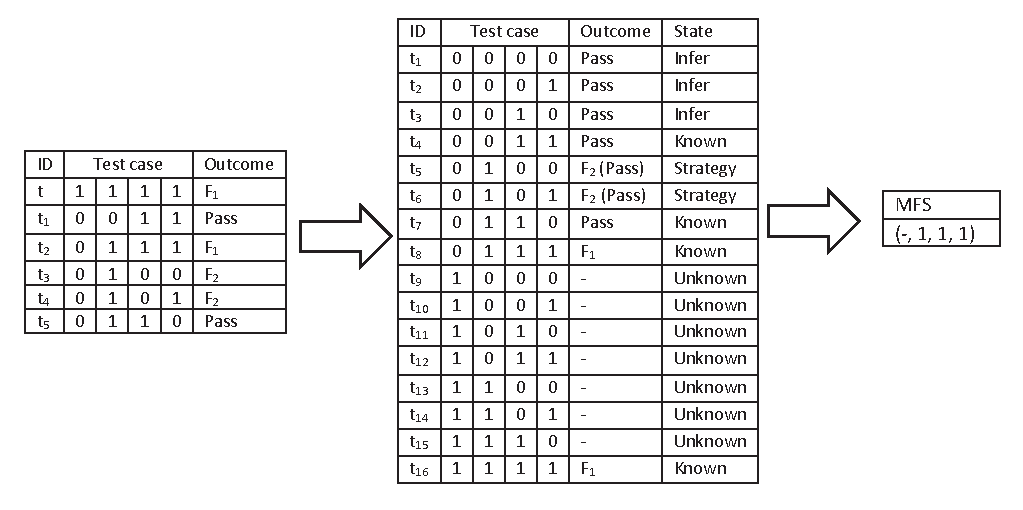
\includegraphics[width=4.99in]{example-of-masking-effects2.eps}
\caption{Masking effects of strategy Distinguishing failures}
\label{fig:maskingeffects2}
\end{figure}


Such deviations from these two strategies are caused by the reduction of the test cases which are known to be failing with specific fault. Here, test cases (0, 1, 0, 0) and (0, 1 0, 1) both triggered other faults, among which the second test case (0, 1, 0, 1) should trigger $F_{1}$ if fault $F_{2}$ was not triggered first, while the first test case not. Hence, neither strategy \emph{Regarded as same failure} nor \emph{Distinguishing failures} can make a perfect determination of the result of these two test cases. Besides this, the incorrect determination of these test cases negatively affect the the inference of FII approach-- FIC\_BS.  For example, with  strategy \emph{Regarded as same failure}, it wrongly inferred the test case $t_{15}$ (1, 1, 1 ,0) to be fail with $F_{1}$ (See the middle part of Fig. \ref{fig:maskingeffects1}), which should be marked as `Unknown' in Table \ref{realMFS-for-11}. With strategy \emph{Distinguishing failures}, however, it marked test case $t_{14}$ (1, 1, 0, 1) as `Unknown' (See the middle part of Fig. \ref{fig:maskingeffects2}), which should be inferred to be fail with $F_{1}$ in Table \ref{realMFS-for-11}.

%\begin{table}[ht]
%\centering
%\tbl{Inferred test cases for two strategies\label{ofot-infer-two}}{
%  \begin{tabular}{ccc}
%\multicolumn{3}{c}{\bfseries  regarded as same failure} \\ \hline
%$\mathcal{T}((-, -, 1, -))$&observed $T_{f}$ &inferred $T_{f}$\\ \hline
%(0, 0, 1, 0)&               & (0, 0, 1, 0) \\
%(0, 0, 1, 1)&               & (0, 0, 1, 1)\\
%(0, 1, 1, 0)&               & (0, 1, 1, 0)\\
%(0, 1, 1, 1)&               & (0, 1, 1, 1)\\
%(1, 0, 1, 0)&               & (1, 0, 1, 0) \\
%(1, 0, 1, 1)&               & (1, 0, 1, 1)\\
%(1, 1, 1, 0)& (1, 1, 1, 0)  & \\
%(1, 1, 1, 1)& (1, 1, 1, 1)  & \\
%\hline
%  \end{tabular}
%  \hspace{1em}
%  \begin{tabular}{ccc}
%\multicolumn{3}{c}{\bfseries  distinguishing failures} \\ \hline
%$\mathcal{T}((1, 1, 1, -))$&observed $T_{f}$ &inferred $T_{f}$\\ \hline
%(1, 1, 1, 0)& (1, 1, 1, 0)  &    ---      \\
%(1, 1, 1, 1)& (1, 1, 1, 1)  &          \\
%\hline
%  \end{tabular}
%  }
%  \end{table}

As masking effect has significant impact on the FII approaches, alleviating this negative effect is desired to improve the quality of the identified MFS.

%\subsection{Summary of the masking effects on the FII approach}
%From the analysis of the formal model, we can learn that masking effect does influence the FII approaches, and even worse, both the \emph{regarded as same failure} and \emph{distinguishing failures} strategies have their own problems in handling this effect. Specifically when compared with the \emph{knowing masking effects} condition, the strategy \emph{regarded as same failure} has a larger possibility of getting more sub-schemas of the actual MFS and getting more schemas which are irrelevant to the MFS, while strategy \emph{distinguishing failures}  may get more super schemas of the MFS and can also get more irrelevant MFS. Note that strategy \emph{regarded as same failure} has a larger chance than \emph{distinguishing failures} at identifying irrelevant schemas. Further, both strategies may ignore the actual MFS with the \emph{distinguishing failures} strategy more likely to ignore the MFS than the \emph{regarded as same failure} strategy.

%Note that our discussion is based on a SUT using deterministic software, i.e., the random failing information of a test case will be ignored. The non-deterministic problem will result in a more complex test scenario, which will not be discussed in this paper.

\section{Test case replacing strategy} \label{sec:method}
The main reason that the FII approach fails to work properly is that it cannot determine $T_{mask(F_{m})}$. In other words, if the test case triggers other unexpected failures which are different from the currently analysed $F_{m}$, it cannot figure out whether this test case will trigger $F_{m}$ because of the masking effects. So to limit the impact of this effect on the FII approach, it is important to reduce the number of test cases that trigger other different failures, as this can reduce the probability that the expected failure may be masked by other different failures.
% strategies cannot accurately identify the MFS is that we cannot figure out the $T(mask_{F_{m}})$.  As $T(mask_{F_{m}}) \subseteq \bigcup_{i = 1 \& i \neq m }^{L}T_{F_{i}}$, in order to weaken the influence of $T(mask_{F_{m}})$, we need to reduce the number of test cases that trigger other failures as much as possible.

For the exhaustive testing model, i.e., $\mathcal{C}(T_{F_{m}})$, as all the test cases will be used to identify the MFS, there is no room left to improve its performance unless we fix other different failures and re-execute all the test cases. However, if only a subset of all test cases is used to identify the MFS (which is how the traditional FII approach works), it is important to make the right selection to limit the size of $T_{mask(F_{m})}$ to be as small as possible.
\subsection{Replacing test cases that trigger unexpected failures}\label{sec:method:describe}
The basic idea is to pick the test cases that trigger other faults and generate new test cases to replace them. The regenerated test cases should either pass in the execution or trigger $F_{m}$.
%The replacement must satisfy the condition that the newly generated ones will not negatively influence the original identifying process.

Normally, when we replace the test case that triggers an unexpected failure with a new test case, we should keep some part of the original test case. We call this part the \emph{fixed part}, and mutate the other part with different values from the original one. For example, assume that a test case (1,1,1,1) triggered an unexpected failure, and the fixed part is (-,-,1,1). Then, we can replace it with a test case (0,0,1,1) which may either pass or trigger the same failure as currently analysed.

The \emph{fixed part} can vary for different FII approaches. For example, for the OFOT \cite{nie2011minimal} algorithm, all parameter values are the fixed part except for the one that needs to be validated, while for the FIC\_BS \cite{zhang2011characterizing} approach, the fixed parts can be dynamically changed, depending on the outcome of the execution of last generated test case.

This replacement process may need to be executed multiple times for one fixed part as it may not always be possible to find a test case that satisfies our requirement. One replacement method is randomly choosing test cases until the satisfied test case is found. While this method may be simple and straightforward, however, it may require many tries. To address this problem and reduce the cost, we propose a replacement approach by computing the \emph{suspiciousness} of the test case with the other faults, and then selecting the test case from a group of candidate test cases that has the least \emph{suspiciousness} with other faults.

% which during the originally test, record the test cases that trigger other test cases and next replacement process will consult this set to avoid some test cases with a high probability to trigger other failures.

To explain the \emph{suspiciousness} notion, we first introduce the \emph{suspiciousness} of a parameter value $o$ with respect to a particular fault $F_{i},  1 \leq i  \leq L$. We use $all(o)$ to represent the number of executed test cases that contain this parameter value, and $f_{i}(o)$ to indicate the number of test cases that trigger the failure of $F_{i}$, and contain this parameter value. Then, the \emph{suspiciousness} of a parameter value \emph{o} with respect to the given fault $F_{i}$, i.e., $\mathcal{SP}(o, F_{i})$, is $\frac{f_{i}(o)}{all(o) + 1}$. This heuristic formula is based on the idea that if a parameter value frequently appears in the test cases that trigger a particular failure, then it is more likely to be an inducing factor that triggers this fault. We add 1 in the denominator for two reasons:  (1)to avoid division by zero when the parameter value has never appeared before, (2)to reduce the bias when a parameter value rarely appears in the test set but coincidentally appears in a failing test case with a particular fault.

Table \ref{suspciousness_example} gives an example to compute the suspiciousness of parameter values with respect to particular faults. The left part of this table gives 4 executed test cases with their outcomes, in which faults $F_{1}$ and $F_{2}$ are triggered. The right part shows the suspiciousness of each parameter value w.r.t. these two faults. Specifically, consider the parameter $P_{1}$ taking value 0. There are three test cases $t_{1}$, $t_{2}$, and $t_{4}$ that contain this parameter value, and only  $t_{2}$ triggered $F_{1}$. Hence, $\mathcal{SP}(P_{1} = 0, F_{1})$ = $\frac{f_{1}(o)}{all(o) + 1}$ = $\frac{1}{3 + 1}$ = 1/4.

\begin{table}[ht]
\centering
\tbl{Suspiciousness example \label{suspciousness_example}}{
  \begin{tabular}{ccc}
ID &  Test cases executed& Outcomes  \\ \hline
$t_{1}$ &(0, 0, 0)& $Pass$ \\
$t_{2}$ &(0, 1, 1)&  $F_{1}$ \\
$t_{3}$ &(1, 1, 0)&  $F_{2}$\\
$t_{4}$ &(0, 1, 1)&  $F_{2}$\\
\hline
  \end{tabular}
  \hspace{1em}
  \begin{tabular}{c|c|ccc}
 \multicolumn{4}{c}{  Suspiciousness for $F1$} \\ \hline
    & $P_{1}$ & $P_{2}$ & $P_{3}$ \\ \hline
 $0$ & 1/4 &  0   & 0 \\
 $1$ &  0  &  $ 1/4 $  & $ 1/3$ \\
\hline
 \multicolumn{4}{c}{  Suspiciousness for $F2$} \\ \hline
 & $P_{1}$ & $P_{2}$ & $P_{3}$ \\ \hline
$0$ & $1/4$  & 0   & $1/3$\\
$1$ & $1/2$  & $1/2$  &  $1/3$ \\
\hline
  \end{tabular}
  }
  \end{table}


With the \emph{suspiciousness} associated with a parameter value, we then define the \emph{suspiciousness} between a test case $t$ and a particular fault $F_{i}$ as:

\begin{displaymath} \mathcal{SP}(t,F_{i})  = \frac{1}{k}\sum_{o \in t} \mathcal{SP}(o, F_{i}) \tag{EQ1} \label{eqn - 00p} \end{displaymath}

where $k$ is the number of parameters in $t$, and $o$ is the specific parameter value in $t$. The \emph{suspiciousness} of a test case w.r.t. a fault is actually the average \emph{suspiciousness} of each parameter value in the test case w.r.t. this fault. For example, considering an unexecuted test case (1, 0, 0). With the suspiciousness of all the parameter values listed in Table \ref{suspciousness_example}, $\mathcal{SP}((1,0,0),F_{1})$ = $1/3 \times (0 + 0 + 0 ) = 0 $ and $\mathcal{SP}((1,0,0),F_{2})$ = $1/3 \times (1/2 + 0 + 1/3 ) = 5/18$.


For a selected test case, we want its ability  to trigger failures of other faults to be as small as possible, such that the masking effects can be alleviated. In practice, the \emph{suspiciousness} varies between test cases and different faults.  As a result, we cannot always find a test case that, for any fault, the \emph{suspiciousness} of this test case w.r.t. that fault is the least.

Table \ref{minimal_maximal} illustrates such a scenario for SUT($2^4$). Suppose the FII approach is analysing MFS for fault $F_{1}$, and needs to replace test case (0,0,0,0) with fixed part (0, -, -, -) that triggers failures of other faults, i.e., $F_{2}$ or $F_{3}$.  This table lists five candidate test cases, with their suspiciousness with $F_{2}$ and $F_{3}$ given in the corresponding columns.  It is obvious that $t_{1}$ has the least suspiciousness with fault $F_{3}$ and $t_{2} $ has the least suspiciousness with $F_{2}$. These two test cases, however, should not be selected because their suspiciousness with another fault is too high. Instead, $t_{3}$ is a good choice as both its suspiciousness with $F_{2}$ and $F_{3}$ is not high (The higher one is just 0.4).

\begin{table}[ht]
\centering
\tbl{Select minimal maximal suspiciousness \label{minimal_maximal}}{
  \begin{tabular}{ccccc}
ID & Candidate test cases& $\mathcal{SP}(t,F_{2})$& $\mathcal{SP}(t,F_{3})$ & $Max\ \mathcal{SP}(t, F_{m}), m = 2,3$ \\ \hline
$t_{1}$ & (0, 0, 0, 1)&     0.7  & 0.2 &   $\mathcal{SP}(t_{1},F_{2})$ : 0.7 \\
$t_{2}$ &(0, 0, 1, 0)&      0.2  & 0.6 &   $\mathcal{SP}(t_{2},F_{3})$ : 0.6\\
$\textbf{t}_{\textbf{3}}$ &\textbf{(0, 0, 1, 1)}&\textbf{0.4} &  \textbf{0.3} & $\textbf{$\mathcal{SP}$(}\textbf{t}_{\textbf{3}},\textbf{F}_{\textbf{2}}\textbf{)}$ : \textbf{0.4}\\
$t_{4}$ &(0, 1, 0, 0)&   0.3 & 0.5  &$\mathcal{SP}(t_{4},F_{3})$ : 0.5\\
$t_{5}$ &(0, 1, 0, 1)&   0.5 & 0.3  &$\mathcal{SP}(t_{5},F_{2})$ : 0.5\\
\hline
  \end{tabular}
  }
  \end{table}

With this in mind, we have to settle for a test case, such that the most likely fault (except for the one that is currently analysed) it can trigger should be the least likely to be triggered when compared with that of other test cases. In other words, we need to find a test case, so that the maximal \emph{suspiciousness} of this test case w.r.t. a given fault is minimized. Formally, we should choose a test case $t$, such that,

\begin{displaymath} \min_{t \in R} \max_{1 \leq i \leq L \& i \neq m}  \mathcal{SP}(t, F_{i}) \tag{EQ2} \label{eqn - 0p}\end{displaymath}

%*******
% F_{m} F_{n} F_{k} needs to be unified
%*******

where $L$ is the number of faults, and $m$ is the current analysed fault. $R$ is the set of all possible test cases that contain the $fixed$ part except those that have been tested. As the $fixed$ part is a set of parameter values which can be deemed as a schema, then obviously $R = \mathcal{T}(fixed)  \backslash T_{executed}$, where $\mathcal{T}(fixed)$ represents all the test cases that contain this fixed part and $T_{executed}$ represents those executed test cases. Additional test cases need to be selected in set $R$, so that FII approaches can work properly.

%We can further resolve this problem. Consider the test case $t$ satisfies \ref{eqn - 0p}. Without loss of generality, we assume that the failure $F_{i}, i \neq m $ is the failure with which the test case $t$ has the maximal \emph{suspiciousness} compared to the other failures. Then, a natural property for $t$ is that $Sp(t, F_{i}) <= Sp(t', F_{i})$, in which test case $t'$ is any other test case which has the maximal suspiciousness with failure $F_{i}$ than other failures.  For example in Table \ref{minimal_maximal}, test cases $t_{1}$,$t_{3}$ and $t_{5}$ have the maximal \emph{suspiciousness} with $F_{2}$ than other failures. Obviously, $ Sp(t_{3}, F_{2}) = 0.4 < Sp(t_{5}, F_{2}) = 0.5 < Sp(t_{1}, F_{2}) = 0.7$.  This property can be formulated as :
%
%\begin{alignat}{2}
%\min\quad &  Sp(t, F_{i}) &{}& \tag{EQ3} \label{eqn - lp}\\
%\mbox{s.t.}\quad
%&t \in R &\quad& {}\nonumber\\
%&Sp(t, F_{i}) > Sp(t, F_{j}), &{}& 1 \leq j \leq L\ \&\ j\neq i, m \nonumber
%\end{alignat}
%
%
%In fact, for each failure $F_{i}, 1 \leq i \leq L \ \& \ i \neq m$, there exists a test case satisfies \ref{eqn - lp}. In other words, for each failure $F_{i}$, exists a test case such that it has the maximal suspiciousness with $F_{i}$ than other failures, and the its suspiciousness with $F_{i}$ is smaller than other test cases which have the maximal suspiciousness with $F_{i}$.  We refer to such test case as $t_{F_{i}}$. Hence to find a test case that satisfies \ref{eqn - 0p}, we just need to find:
%
%\begin{alignat}{2}
%\min\quad &  t_{F_{i}} &{}& \tag{EQ4} \label{eqn - 2p}\\
%\mbox{s.t.}\quad
%& 1 \leq i \leq L \ \& \ i \neq m &\quad& {}\nonumber
%\end{alignat}
%
%Going back to the example in Table \ref{minimal_maximal}, $t_{F_{2}}$ is $t_{3}$ and $ t_{F_{3}}$ is $t_{4}$. As $Sp(t_{3}, F_{2}) = 0.4 < Sp(t_{4}, F_{3}) = 0.5$, $t_{3}$ is a better choice.

%According to \ref{eqn - 2p}, to determine such a test case lies in solving \ref{eqn - lp} because if it is solved we just need to rank the one that has the minimal value from the solutions to \ref{eqn - lp}. For example in Table \ref{minimal_maximal}, $Sp(t_{3}, F_{2})$ is the minimal when comparing with that of other test cases ($t_{1}$, $t_{5}$) has the maximal suspiciousness with $F_{2}$, while $Sp(t_{4}, F_{3})$ is the minimal for $F_{3}$. As $Sp(t_{3}, F_{2}) < Sp(t_{4}, F_{3})$, $t_{3}$ is better choice.
%
%As to \ref{eqn - lp}, it can be formulated as an 0-1 integer linear programming (ILP) problem. Assume the SUT has $K$ parameters in which the $i$th parameter has $V_{i}$ values. And the SUT has $L$ failures. We then define the variable $x_{i,j}$ as:
%\begin{displaymath}
%x_{i,j} = \begin{cases}1 & the\ \emph{i}th\ parameter\ of\ the\ test\ case\  take\ the\ \emph{j}th\ value\ for\ that\ parameter\\0 & otherwise\end{cases}
%\end{displaymath}
%We then take $Sp((i,j), F_{m})$ to be the \emph{suspiciousness} between the \emph{j}th value of the \emph{i}th parameter of the SUT and the failure $F_{m}$. A set $Fix$ of parameter values to define the fixed part in the test case we should not change, i.e., $Fix = \{(i, j)\ |\ i\ is\ the\ fixed\ parameter\ in\ the\ test\ case, j\ is\ the\ corresponding\ value\}$. As we can generate redundant test cases, so we keep a test set $T_{executed}$ to guide the generation of different test cases. Then \ref{eqn - lp} can be transformed into following ILP formula:
%
%\begin{alignat}{2}
%\min\quad & \frac{1}{|K|}\sum_{i = 0}^{K-1}\sum_{j = 0}^{V_{i}-1} Sp((i,j), F_{m}) \times x_{i,j} &{}& \tag{EQ5} \label{eqn - 3p}\\
%\mbox{s.t.}\quad
%& 0 \leq x_{i,j} \leq 1 &\quad& { i = 0 .. K - 1, j = 0,.. V_{i} - 1 }\\
%&  x_{i,j} \in  \mathbb{Z}&\quad& { i = 0 .. K - 1, j = 0,.. V_{i} - 1 }\\
%& \sum_{j = 0}^{V_{j}-1} x_{i,j} = 1&\quad& { i = 0 ... K - 1}\\
%&  x_{i,j} = 1 &\quad& { (i,j) \in Fix }\\
%& \sum_{i = 0}^{K-1}\sum_{j = 0}^{V_{i}-1} (Sp((i,j), F_{m}) - Sp((i,j), F_{m'}) ) \times  x_{ij} \geq 0 &\quad& {1 \leq m'  \leq L, m' \neq m}\\
%& \sum_{i = 0}^{K-1}  x_{i,t[i]} < K &\quad& {t \in T_{executed}}
%\end{alignat}
%
%In \ref{eqn - 3p}, constraints (1) and (2) indicate that the variable $x_{i,j}$ is a 0-1 integer. Constraint (3) indicates that a parameter in one test case can only take on one value. Constraint (4) indicates that the test case should not change values of the fixed part. Constraint (5) indicates that the suspiciousness between the test case and failure $F_{m}$ is higher than that of the other failures. In Constraint (6), $t[i]$ indicates the value of the $i$th parameter of test case $t$ in $T_{executed}$. Hence, this constraint points out that the test cases generated should not be the same as the test cases in $T_{executed}$.

%As we have formulated the problem into a 0-1 integer programming problem, we just need to utilize an ILP solver to solve this formula.
%\ref{eqn - 0p} can be further converted into an integer satisfaction and optimization problem (Details in Section \ref{sec:appendixs:covert} in the Appendix),
% As \ref{eqn - 0p} is actually an integer satisfaction and optimization problem, we can utilize an ILP solver to solve this problem. In this paper, we use the solver introduced in \cite{Berkelaar2004}, which is a mixed Integer Linear Programming (MILP) solver suitable for satisfaction and optimization problems.
The complete process of replacing a test case with a new one while keeping some fixed part is depicted in Algorithm \ref{alg:one}.

\begin{algorithm}[ht]
%\SetAlgoNoLine
\KwIn{ fault $F_{m}$, all the candidate test cases $R$, the suspiciousness matrix $\mathcal{SP}$}
\KwOut{ $t_{new}$ the regenerate test case }
%$index$ = 0; $FreNum_{\alpha}$ = -1\;
\While{\textbf{not} $R$ is empty }{
       $t_{new} \leftarrow \min_{t \in R} \max_{1 \leq i \leq L \& i \neq m}  \mathcal{SP}(t, F_{i})$\;
       $result \leftarrow execute(t_{new})$\;
       $R \leftarrow R \backslash t_{new} $\;
       $update\_SP(t_{new})$ \;
        \eIf  {$result == PASS\ or\ result ==  F_{m}$}{
         \Return $t_{new}$\;
           }{
         continue\;
         }
       }
       \Return \emph{null}

\caption{Replacing test cases triggering unexpected failures}
\label{alg:one}
\end{algorithm}
%
%
The inputs to this algorithm consist of the fault $F_{m}$ under analysis, the candidate test cases $R = \mathcal{T}(fixed)  \backslash T_{executed}$  and the suspiciousness matrix $\mathcal{SP}$, which records the suspiciousness of each factor $o$ with respect to each fault $F_{i}$, i.e., $\mathcal{SP}(o, F_{i})$ ($1 \leq i \leq L $). The output of this algorithm is a test case $t_{new}$ which either triggers the expected $F_{m}$ or passes.

The outer loop of this algorithm (lines 1 - 11) contains three parts:

The first part (lines 2 - 3) generates and executes a new test case which is supposed to be least likely to trigger faults different from $F_{m}$. The new test case is generated according to \ref{eqn - 0p}. In our implementation,  we use the solver introduced in \cite{Berkelaar2004}, which is a mixed Integer Linear Programming (MILP) solver suitable for satisfaction and optimization problems. (Note that a simpler linear search algorithm can also be applied in our approach to find a proper test case. However, as the problem to search a proper test case is related to Integers (a test case consists of discrete parameters with discrete values), we use Integer Linear Programming (ILP) technique instead.) When a test case is generated, we remove it from the candidate test case set $R$ to avoid redundancy (line 4).

The second part (line 5) updates the suspiciousness matrix ($\mathcal{SP}$) for each parameter value that is involved in this newly generated test case (line 5). Specifically, for a particular parameter value $o$, the number of executed test cases that contain $o$, i.e., $all(o)$, increases by 1. Additionally, if this test case triggers failure of $F_{i}$ ($1 \leq i \leq L $) , then the number of test cases that contain $o$ and trigger failure of $F_{i}$, i.e., $f_{i}(o)$, increases by 1. At last, the suspiciousness value will be re-computed according to formula $\mathcal{SP}(o, F_{i}) = \frac{f_{i}(o)}{all(o) + 1}$ ($1 \leq i \leq L $).

% basic idea for this part is to search each failure different from $F_{m}$ (line 3) and find the best test case that has the least suspiciousness with other failures. In detail, for each failure we set up an ILP solver (line 4) and use it to get an optimal test case for that failure, i.e., $t_{F_{i}},1 \leq i \leq L\ \&\ j\neq m$, according to \ref{eqn - lp} (line 5). We compare the optimal value for each failure, and choose the one with less suspiciousness with other failures (lines 6 - 9).

The last part (lines 6 - 10) checks whether the newly generated test case is as expected. Specifically, if the test case passes or triggers the same failure of fault -- $F_{m}$, a satisfied test case is obtained (line 6) and returned (line 7). Otherwise, we will repeat the process, i.e., generate a new test case and check again (lines 8 - 9).

%Note that the ending condition of this  algorithm has another exit, besides finding an expected test case (line 6), which is when the function \emph{MeetEndCriteria()} returns \emph{true} (line 1). We did not explicitly show function \emph{MeetEndCriteria()}, because this is dependent on the computing resource and the desired accuracy. In detail, if we want to get a high quality result and have enough computing resource, it is desirable to try many times to get the expected test case; otherwise, a relatively small number of attempts to find a proper test case is recommended.

%In this paper, we just set 3 as the greatest number of iterations for this function. When it ends with \emph{MeetEndCriteria()} returning true, it will return null (line 18), which means we cannot find an expected test case.



\section{Illustration of the approach}\label{sec:appraoch}

This section will illustrate the complete MFS identification approach that combines the traditional MFS identification procedure with test cases replacement strategy.

%which give a description for the MFS identification with the test cases replacement operation. Before we talk about this, let us first recall the basic theory for the MFS identification.
%
%\subsection{MFS identification}
%
%fixed part is that . The additionl test case just need to maintain the fixed part.


\subsection{MFS identification with replacement strategy}

Algorithm \ref{alg:two} shows the procedure of our approach. The inputs to this algorithm are the fault $F_{m}$ that is currently focused on and an original failing test case $t$. The output of this algorithm is to give the MFS for fault $F_{m}$ in the test case $t$. Variable $\mathcal{SP}$ is to record the suspicious value between each parameter value with each fault. $T_{Unknown}$ is the set of test cases that is not yet determined to be fail with fault $F_{m}$ or not, and $T_{F-Known}$ is the set of test cases that are deemed to trigger the fault $F_{m}$. This algorithm loops until some MFS are determined (line 25 - 27). This is based on Lemma \ref{pro:dsmfs} in Section 3.3. Specifically,  by computing the minimal schemas of $T_{F-Known}$, i.e., $\mathcal{C}(T_{F-Known})$, and minimal schemas of $T_{F-Known} \bigcup T_{Unknown}$, i.e., $\mathcal{C}(T_{F-Known} \bigcup T_{Unknown})$, respectively, we can determine $\mathcal{C}(T_{F-Known})$ are MFS if they are contained in $\mathcal{C}(T_{F-Known} \bigcup T_{Unknown})$.

In each iteration,  this algorithm will generate one additional test case (line 7) to execute. This test case is randomly selected from a candidate set $R$ which has the same fixed part (line 6). The fixed part is different in each iteration.
%(See Algorithm \ref{alg:fic} in the Appendix for detail)
Then the approach will execute this test case (line 8) and update the suspiciousness matrix (line 9) according to the execution result. If the result is pass or fail with the same fault $F_{m}$, then the generated test case is a proper test case for MFS identification; otherwise, we should run the replacement strategy (line 10 - 15) based on Algorithm \ref{alg:one}. Note that if we cannot find a proper test case by Algorithm \ref{alg:one}, we need to randomly select one test case in $R$ (line 13), and regard it as fail with $F_{m}$ (line 14). Next we will infer the result of some unknown test cases according to the result of the generated test case $t_{next}$ (line 17 - 24). This inferring procedure is exactly based on corollaries \ref{lemma:inferpassing} and \ref{lemma:inferfailing}. After that, we update the $T_{F-known}$ and $T_{Unknown}$ (line 19 - 20, line 23), and re-check if the ending condition is satisfied (line 27).

\begin{algorithm}[ht]
%\SetAlgoNoLine
\KwIn{ fault $F_{m}$, original failing test case $t$ }
\KwOut{ $MFS$ returning the determined MFS }
%$index$ = 0; $FreNum_{\alpha}$ = -1\;

$\mathcal{SP} \leftarrow init\_Suspicious\_Matrix(t)$ \;
$T_{Unknown} \leftarrow  T_{ALL} \setminus t $ \;
$T_{F-Known} \leftarrow \{ t \} $ \;
$MFS \leftarrow empty$ \;
\While{ $true$}{
%       $optimal \leftarrow MAX$,
%       $t_{new} \leftarrow null$ \;
%       \ForAll {$F_{i} ( i = 1, ... m-1 , m+2,...L )$}{
%                $solver \leftarrow setup(Param, fixed, T_{executed}, F_{i}, Sp)$\;
%               \DontPrintSemicolon $(optimal', t_{new}') \leftarrow solver.getOptimalTest()$; \tcc*[f]{Use ILP solver to get $t_{F_{i}}$} \;
%                \If (\tcc*[f]{Select $t_{F_{i}}$ which has smaller suspiciousness}){$optimal' < optimal$}{
%                       $t_{new} \leftarrow t_{new}'$\;
%                       $optimal \leftarrow optimal'$\;
%                    }
%          }
       $ R \leftarrow  \mathcal{T}(current\_fixed\_part)$ \;
       $t_{next} \leftarrow random\_pick(R)$\;
       $result \leftarrow execute(t_{next})$\;
       $update\_SP(t_{next})$ \;
        \If  {$result \neq PASS\ and \ result \neq  F_{m}$}{
         $t_{next} \leftarrow Replacing(F_{m}, \mathcal{SP}, R) $\;
          \If  {$t_{next}  ==  null$}{$t_{next} \leftarrow random\_pick(R)$\;
          $result \leftarrow F_{m}$}{}
           }{ }
            \eIf  {$result == F_{m}$}{
           $T_{infer-F} \leftarrow InferringFailing (t_{next}, SV) $\;
           $T_{F-Known} \leftarrow T_{F-Known} \bigcup t_{next} \bigcup T_{infer-F}$\;
           $T_{Unknown} \leftarrow T_{Unknown} \setminus (t_{next} \bigcup T_{infer-F}) $ \;
           }{ $T_{infer-P} \leftarrow InferringPassing (t_{next}, SV) $\;
           $T_{Unknown} \leftarrow T_{Unknown} \setminus  (t_{next} \bigcup T_{infer-P}) $ \;}


           $MFS \leftarrow \mathcal{C}(T_{F-Known})$ \;
           $M_{Possible} \leftarrow \mathcal{C}(T_{F-Known} \bigcup T_{Unknown})  $ \;
            \If{ $ MFS \subseteq M_{Possible} $}{break\;}{}

       }
       \Return $M_{Candidate}$

\caption{MFS identification with Replacing test cases strategy}
\label{alg:two}
\end{algorithm}



\subsection{A case study using the replacement strategy}\label{sec:method:case}
%Next we will take the FII approach--OFOT algorithm as the subject to see how our approach works on them.

In this section, we will give a case study to illustrate our approach. Suppose we want to test a system with eight parameters, each of which has three options, i.e., SUT($3^8$). When we execute the test case $t_{0}$ -- (0, 0, 0, 0, 0, 0, 0, 0), a failure of fault--$e1$ is triggered. Furthermore, there are two more potential faults, $e2$ and $e3$, that may be triggered during the testing and they will mask the desired fault $e1$. Next, we will use FIC\_BS \cite{zhang2011characterizing} with replacement strategy to identify the MFS of $e1$.  The process is shown in Figure \ref{fig:fci_case_study}. In this figure, there are two main columns. The left main column indicates the executed test cases during testing as well as the executed results, with each executed test case corresponding to a specific label, $t_{1}$ -- $t_{8}$, at the left. The underline part for each test case is the $fixed$ part according to FIC\_BS \cite{zhang2011characterizing}.  The right main column lists the suspiciousness matrix when a test case triggers $e2$ or $e3$.  The executed test case, shown in bold, indicates the one that triggers the failure of other faults and should be replaced in the next iteration.
%In detail, the matrix records the suspiciousness between each parameter (Columns $P1$ -- $P8$) for each value it can take (Column v) with the unexpected failure (Column F).
%%the test case which are labeled with a deleted line represent the original test case generated by OFOT, and it will be replaced by the regenerated test case which are labeled with a wave line under it.
\begin{figure}[htbp]
\centering
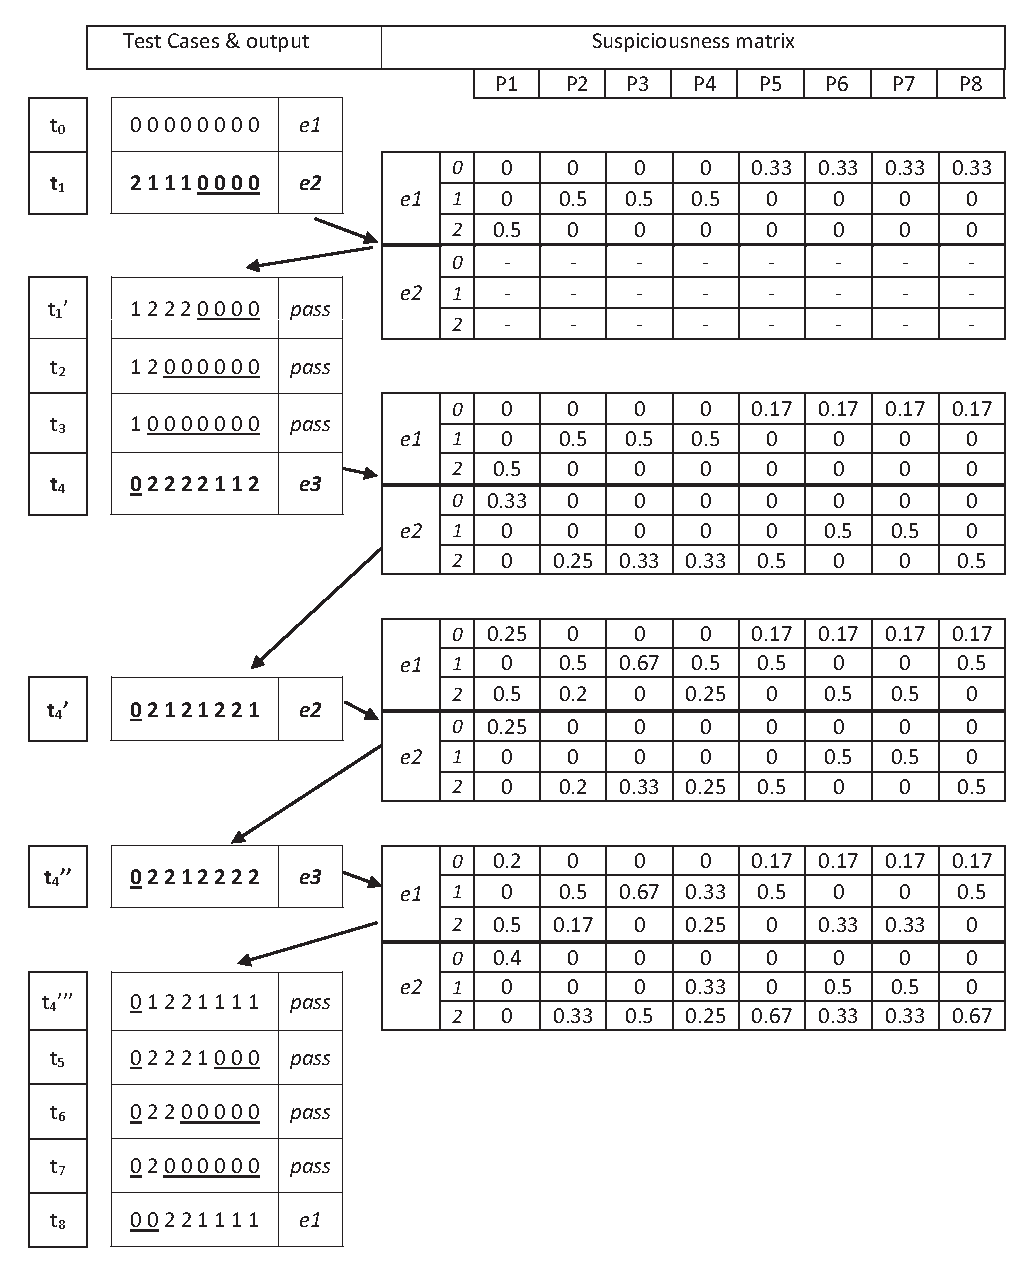
\includegraphics[width=4.31in]{table.eps}
\caption{A case study using our approach}
\label{fig:fci_case_study}
\end{figure}

The completed MFS identifying process listed in Figure \ref{fig:fci_case_study} works as follows. Firstly the original FII approach determines which $fixed$ part needed to be tested in each iteration. Then an extra test case will be generated to fill in the remaining part. After executing the extra test case, if the execution did not trigger any unexpected faults ($e_{2}, e_{3}$), the original FII process will continue until the MFS is identified. Otherwise,  the replacement strategy starts when an unexpected failure of other faults is triggered. The replacement process will mutate the parameter values that are not in the $fixed$ part according to \ref{eqn - 0p}. After the replacement process, the control for the MFS identifying process will be passed back to the original FII approach.  Next we will specifically explain how the replacement works with an example in Figure \ref{fig:fci_case_study}.

From Figure \ref{fig:fci_case_study}, for the test case that triggered $e2$ -- (2, 1, 1, 1, 0, 0, 0, 0) (in this case, the fixed part of the test case is (-, -, -, -, 0, 0, 0, 0), in which the last four parameter values are the same as the original test case $t_{0}$), we generate the related matrix at left. Each element in this matrix is computed according to \ref{eqn - 00p}. All the suspiciousness with $e3$ is labeled with a short slash as there is no test case triggering this fault in this iteration.  After this matrix is determined, we can obtain the optimal test case with the ILP solver, which is $t_{1}'$--(1, 2, 2, 2, 0, 0, 0, 0), with its suspiciousness 0.167, which is smaller than all other test cases.

This replacement process is started each time a new test case triggered another fault until we finally get a proper test case. Sometimes we could not find a satisfied replacement test case in just one trial like $t_{1}$ to $t_{1}'$.  When this happens, we need to repeat searching for the proper test case. For example, for $t_{4}$ which triggered $e3$, we tried three times-- $t_{4}', t_{4}'', t_{4}'''$ to finally get a satisfied $t_{4}'''$ which passes the testing. Note that the \emph{suspiciousness} matrix continues to change as the test case is generated and executed so that we can adaptively find an optimal one.

With the replacement test cases, the FII approach can work properly. At last, the MFS identified for fault $e1$ is (0,0, -, -, -, -, -, - ) (Test cases passed when we mutated the first two parameter values of the original failing cases). Note that, we did not show the complete process to obtain the MFS (0, 0, -, -, -, -, -, -). This is because we need to list all the possible test cases ($3^8 = 6561$ test cases in total) to illustrate this process, which is not possible in this paper.

Another notable point is that, in this example, test cases that trigger $e2$ and $e3$ do not contribute to the MFS identification. In a real-world scenario, however, it is appealing to iteratively start MFS identification for $e2$ and $e3$ based on these test cases.

%\subsection{Complexity analysis}
%The complexity of our approach relies on two variables: the number of test cases that triggered other failures which need to be replaced, and the number of test cases that need to be tried to generate a non-masking-effect test case. The complexity is the product of these two variables.
%
%The first variable is dependent on the extra test cases that are needed to identify the MFS, and this number varies in different FII approaches. Table \ref{extra-testcases-complexisty} lists the number of test cases that each algorithm needed to get the MFS, where \emph{d} indicates the number of MFS in the SUT. \emph{k} means the number of the parameters of the SUT. \emph{t} is the degree of MFS in the SUT. \emph{c} is an upper bound, and satisfies $d \leq \frac{c}{2} loglog k$. \emph{v} is the number of values that a parameter can take.
%
%\begin{table}
%\centering
%\tbl{The number of test cases each FII approach needed to identify MFS\label{extra-testcases-complexisty}}{
%  \begin{tabular}{c | c} \hline
%\bfseries Method & \bfseries number of test cases to identify MFS\\ \hline
%Charles ELA & depends on the  covering array \\
%Martinez with safe value \cite{martinez2008algorithms,martinez2009locating} & $O(\hat{d}log k + \hat{d}^{2})$ \\
%Martinez without safe values \cite{martinez2008algorithms,martinez2009locating} & $O(d^{2} + dlog k + log^{c} k)$  \\
%Martinez' ELA \cite{martinez2008algorithms,martinez2009locating} &  $O(ds^{v}log k)$\\
%Shi SOFOT \cite{shi2005software}& $O(k)$ \\
%Nie OFOT \cite{nie2011minimal} & $O(k \times d)$\\
%Ylimaz classification tree & depends on the  covering array\\
%FIC \cite{zhang2011characterizing} &  $O(k)$ \\
%FIC\_BS \cite{zhang2011characterizing}& $O(t(log k + 1) + 1)$\\
%Ghandehari's suspicious based  \cite{ghandehari2012identifying}& depends on the number and size of MFS\\
%TRT \cite{niu2013identifying}&  $O(d\times t \times log k + t^{d})$\\ \hline
%  \end{tabular}
%  }
%  \end{table}
%
%Note that each algorithm may have some restrictions, details of which are shown in \cite{zhang2011characterizing}.
%
%To get the magnitude of the second variable, we need to figure out the probability of a test case that could trigger other failure. The first consideration is the \emph{fixed} part, as the additional generated test case should somehow contain this part. As mentioned before, we can generate $(v-1)^{k - p} $  (\emph{p} is the number of parameter values in the \emph{fixed} part) possible test cases that contain the \emph{fixed} part. Apart from the one that needs to be replaced, there remain $(v-1)^{k - p}- 1$ candidate test cases, which indicates the complexity is $O((v-1)^{k - p} - 1)$. However, to avoid the exponential computation, we use the $MeetEndCriteria()$ function to end Algorithm 1 when the attempts to find a proper test case is over a prior given constant, say $N$, so the complexity for the second part is $O( min (N, (v-1)^{k - p} - 1))$.
%%
%%While for adaptive approach, as the $\emph{fixed}$ part is derived from the existed failing test case, which in fact make the test cases to be selected one more less (the existed one), so the complexity is  $O(v^{k - p} - 2)$.
%
%We note that exponent $k - p$ has a significant effect on the complexity of the second value. The greater $p$ is, the less test cases that can be generated. Different approach has different $p$. For example, for the OFOT approach, $p$ is equal to $k - 1$.  And for the FIC\_BS approach, $p$ varies ranging from $k-1$ to $1$. While for the non-adaptive approaches, as the $fixed $ part is commonly the schemas that are needed to be covered, so the $p$ for these approaches is at least equal to $t$. We have listed all of them in Table \ref{fixed-part-complexisty}. It is noted that the approach $Martinez\ without\ safe values$ has no such complexity, because it works when $v = 2$, and this results in not having other test cases to be replaced if we test a fixed part when triggering other failures.
%
%\begin{table}
%\centering
%\tbl{The complexity of the second part\label{fixed-part-complexisty}}{
%  \begin{tabular}{c | c} \hline
%\bfseries Method & \bfseries fixed part\\ \hline
%Charles ELA &   $O( min (N, (v - 1)^{k - t} - 1))$\\
%Martinez with safe value \cite{martinez2008algorithms,martinez2009locating} &$O( min (N, (v-1) - 1)) \sim O( min (N, (v-1)^{k - 1} - 1))$\\
%Martinez without safe values \cite{martinez2008algorithms,martinez2009locating} &$ - $  \\
%Martinez' ELA \cite{martinez2008algorithms,martinez2009locating} & $O( min (N, (v - 1)^{k - t} - 1))$\\
%Shi SOFOT \cite{shi2005software}& $O( min (N, (v-1) - 1))) $\\
%Nie OFOT \cite{nie2011minimal} & $O( min (N, (v-1) - 1)))$\\
%Ylimaz classification tree & $O( min (N, (v - 1)^{k - t} - 1)$\\
%FIC \cite{zhang2011characterizing} &  $O( min (N, (v-1) - 1)) \sim O( min (N, (v-1)^{k - 1} - 1))$\\
%FIC\_BS \cite{zhang2011characterizing}& $O( min (N, (v-1) - 1)) \sim O( min (N, (v-1)^{k - 1} - 1))$\\
%Ghandehari's suspicious based  \cite{ghandehari2012identifying}&$ O( min (N, (v - 1)^{k - t} - 1))$\\
%TRT \cite{niu2013identifying}&$ O( min (N, (v-1) - 1)) \sim O( min (N, (v-1)^{k - 1} - 1)) $\\ \hline
%  \end{tabular}
%  }
%  \end{table}
%
%Above all, the cost of replacement strategy varies in different FII approaches. Note that this cost is computed for the worst case, and in practice much less test cases are needed to identify the MFS. This is because first, not every test case generated by the FII approach needs to be replaced; and second, a satisfied test case can usually be found before the whole searching space is explored. From complexity analysis, in fact, we cannot determine which approach is better than others, as the cost of each approach is dependent on different factors. For example in Table \ref{extra-testcases-complexisty}, the extra test cases needed for OFOT\cite{nie2011minimal} and FIC\_BS\cite{zhang2011characterizing} are $O(k \times d)$ and $O(t(log k + 1) + 1)$ , respectively. Values $t$, $k$ and $d$ determine which one is better in practice. So for different SUT with different MFS, which FII approach is better can be completely changed. Besides, the less cost in practice is not always good for identifying MFS.  A potential problem is, with less candidate test cases, the replacement strategy may not find a satisfied test case, which will result in a low quality of the identified schemas.


%we can find that  the worst is . However, this is not means that it , because the less candidate cases also can give a less chance to get the satisfied test case.  In this paper, we choose the FII BS as the candidate, because it can probably, and its test cases are less, but, it is not necessary the best, because these approaches has its own restrictions. And in some partucal, For example, if there are overlapped, a better choice is TRT \cite{niu2013identifying}.

%The production of this two complexity is the final complexity for our approach. This result is a upper bond, most times the system will just contain small size of failures which will significantly not reach this bond. Also, if a system with too many bugs that make the replacement too costly will just need to rewrite instead of identifying. Further more our "suspicious set" will largely reduce the replacement cost comparing with previous work, which will be validated in the empirical study later.
%
%This complexity is well lay on the number of failures and the magnitude and location of the MFS of each schema, we only analysis the average performance of our approach. Also this approach also lay on the number of tests need to be executed about each algorithm.

\section{Discussion about the influence of the assumptions}\label{sec:assumptions}

In section \ref{sec:introd:mfs}, we introduced three assumptions that can simplify our formal modeling and proposed approach, and in section \ref{subsec:Formal:identi}, we introduced the safe value assumption which can reduce the number of test cases to identify MFS. In this section, we will discuss their influence on our propositions and approach, as well as some measures to alleviate their impact.

\subsection{Deal with non-deterministic problem}
The first assumption is that the outcomes of all the tests are deterministic. In practice, re-executing the same test case may result in different outcomes. For example, if the program using some random variables, different runs of the test case will assign different values to these random variables. As a result, the control flow of the program may be changed and hence the outcome will be different. We called this type of failure the non-deterministic failure \cite{yilmaz2006covering,fouche2009incremental}. Non-deterministic failure will complicate the MFS identification, and even worse, it may lead to an unreliable result of the MFS identification. Consider the the following example in Table \ref{non-deterministic-example}, the only difference between the left and the right test set is the outcome of test case (0, 1, 1). This subtle difference leads to different results of the MFS identification. Hence, if there is one or more test cases which have non-deterministic executing results, the MFS identification is not reliable.
 \begin{table}[ht]
\centering
\tbl{MFS of two similar test sets\label{non-deterministic-example}}{
   \begin{tabular}{c c  c }
$T_{fail}$ &$T_{pass}$ &  $MFS$\\ \hline
 (0, 0, 0) &           &  (0, 0, -)\\
 (0, 0, 1) &           &  (0, -, 0)\\
 (0, 1, 0) &           & \\
           & (0, 1, 1) & \\
           & (1, 0, 0) & \\
           & (1, 0, 1) & \\
           & (1, 1, 0) & \\
           & (1, 1, 1) & \\
\hline  \end{tabular}
  \hspace{1em}
   \begin{tabular}{c c  c }
$T_{fail}$ &$T_{pass}$ &  $MFS$\\ \hline
 (0, 0, 0) &           &  (0, -, -)\\
 (0, 0, 1) &           &  \\
 (0, 1, 0) &           & \\
 (0, 1, 1) &           & \\
           & (1, 0, 0) & \\
           & (1, 0, 1) & \\
           & (1, 1, 0) & \\
           & (1, 1, 1) & \\
\hline  \end{tabular}
  }
  \end{table}

Inspired by the idea that using multiple same-way covering arrays to identify the MFS \cite{fouche2009incremental}, one potential solution to alleviate this non-deterministic failure is by adding redundancy, i.e., through re-executing the same test case to obtain the relatively stable outcome. However, this measure will increase the overall cost of the MFS identification, so the tradeoff between cost and the quality of MFS identification should be further studied.

\subsection{Deal with failures distinguishing problem}
The second assumption is that different errors in the software can be easily distinguished by information such as exception traces, state conditions, or the like. If we cannot directly distinguish them, our approach does not work. This is because we cannot determine which test case should be replaced and with what. In such case, one potential solution is to use the clustering techniques to classify the failures according to available information \cite{zheng2006statistical,jones2007debugging,podgurski2003automated}. If we cannot classify them because we do not have enough information (e.g., the black box testing) or it is too costly, we believe the only approach is to take the \emph{regarded as same failure} strategy. With this strategy, we must aware that the MFS identified are likely to be sub-schemas or irrelevant schemas of the actual MFS. Note that in the next section, all the failures can be distinguished from each other according to the exception traces in our experiments.

\subsection{Deal with inter-option constraints}
The third assumption is that all the test cases are valid, i.e., SUT does not have any inter-option constraint. This is a very strong assumption. In this section, we will try to remove this assumption. In fact, with constraints known in prior, many studies in CT have proposed approaches to avoid them when generating test cases \cite{cohen2007exploiting,cohen2007interaction,cohen2008constructing,calvagna2008logic,yu2013efficient,petke2013efficiency,yu2015constraint}.
Generally, with constraints known in prior, not all test cases in the SUT are valid.  We use $T_{valid}$ to denote those valid test cases, i.e., test cases that do not contain any of the constraints. Hence, the test cases we generated for MFS identification or replacement are limited to those in $T_{valid}$. Note that this can also make MFS identification invalid. For example, in Table \ref{MFS-with-constriants}, assume test case(0, 1, 1) is invalid. Then without any more information, we cannot determine the MFS (See two different results in Table \ref{non-deterministic-example}).

\begin{table}[ht]
\centering
\tbl{MFS identification with constraints\label{MFS-with-constriants}}{
   \begin{tabular}{c c c c }
$T_{fail}$ &$T_{pass}$ &  $T_{invalid}$ \\ \hline
 (0, 0, 0) &           &             \\
 (0, 0, 1) &           &             \\
 (0, 1, 0) &           &             \\
           &           &  (0, 1, 1)  \\
           & (1, 0, 0) &             \\
           & (1, 0, 1) &             \\
           & (1, 1, 0) &             \\
           & (1, 1, 1) &             \\
\hline  \end{tabular}
  }
  \end{table}


Another type of constraint includes those that can not be found at first, but triggered a failure later in testing\cite{yilmaz2013reducing}. The same as the approach proposed in \cite{yilmaz2013reducing}, we can just treat them as one type of failure, and then use the MFS identification approach to identify them when encountering any invalid test cases.

\subsection{Deal with safe values}
The last assumption is the safe value, i.e., each parameter has one value that is not the part of any MFS. With this assumption, based on corollaries \ref{lemma:inferfailing} and \ref{lemma:inferpassing}, we can infer the result of many test cases without executing them. On the contrary, if this assumption does not hold, those test cases may be inferred incorrectly. As a result, the MFS that identified by FII approaches are not accurate.

In theory, to solve this problem, we should exhaustively execute all the test cases of which the results could be inferred. This is a costly process, and hence, some approaches have been proposed to handle such problem.  Mart{\'\i}nez \cite{martinez2008algorithms,martinez2009locating} proposed two approaches without the safe value assumption, but both of them needs to know the number of MFS or the degrees of them in prior. Then either through generating higher-way covering array or adaptively generating additional test case, they can determine the MFS. We \cite{niu2013identifying} have also proposed an approach to alleviate this problem. In that work, we repeatedly check the same schema to reduce the impact of non-safe values.

\section{empirical studies}\label{sec:emprical}
To investigate the impact of masking effects on FII approaches in real software testing scenarios and to evaluate the performance of our approach in handling this effect, we conducted several empirical studies. Each of the studies focuses on addressing one particular issue, as follows:

%In this section, we conducted several empirical studies to address the following questions:
\textbf{Q1}: Do masking effects exist in real software that contains multiple faults?

\textbf{Q2}: How well does our approach perform compared to traditional approaches?

\textbf{Q3}: Is the ILP-based test case searching technique efficient compared to the random selection?

\textbf{Q4}: Compared to the masking effects handling approach FDA-CIT \cite{yilmaz2013reducing}, does our approach have any advantages ?
%et improvement in handling effects and limiting the costs(reducing extra test cases).

%\textbf{Q5}: Does voting system that consists of different approaches can make improvements?
%
%Specifically, section 6.1 surveyed several open-source software to gain a insight of the existence of multiple faults and their masking effects. Section 6.2 directly applied three MFS-identifying programs on the surveyed software and analysis their results. Section 6.3 applied our approach on the software and a comparison with traditional approaches will be discussed. Section 6.4 discuss the threats to validity of our empirical studies.

\subsection{The existence and characteristics of masking effects}\label{sec:emprical:exist}
In the first study, we surveyed three kinds of open-source software systems to gain an insight into the existence of multiple faults and their effects. The software under study were HSQLDB, JFlex and Grep. The first is a database management software written in pure Java, the second is a lexical analyser generator, and the last one is a command-line utility for searching plain-text data sets for lines matching a regular expression.  The reason that we chose these systems is because they  contain different versions and are all highly configurable so that the options and their interactions can affect their behaviour. Additionally, they all have a developer community so that we can easily obtain the real bugs reported in the bug tracker forum. Table \ref{software description} lists the program, the versions surveyed, number of lines of code, number of classes in the project, and the bug's ids \footnote{ http://sourceforge.net/p/hsqldb/bugs \\
http://sourceforge.net/p/jflex/bugs \\ http://savannah.gnu.org/bugs/ } for each of the software.

%\begin{table}\renewcommand{\arraystretch}{1.3}
%\caption{Software under survey}
%\label{software description}
%
%\end{table}
%\begin{table}\renewcommand{\arraystretch}{1.3}
%\tbl{Software under survey\label{software description}}{
%\begin{tabular}{c|c|c|c|c} \hline
%software & versions & LOC & classes & bug pairs\footnote{ http://sourceforge.net/p/hsqldb/bugs
%http://sourceforge.net/p/jflex/bugs  } \\ \hline
%
%HSQLDB  &2.0rc8 & 139425 & 495 &  \#981 \& \#1005\\
%	   &2.2.5 & 156066 & 508 & \#1173 \&  \#1179\\
%	    &2.2.9 & 162784 &525 & \#1286 \& \#1280\\
%JFlex  &1.4.1 &  10040 &58 & \#87 \& \#80 \\
%      &1.4.2 &  10745 &61 &  \#98 \& \#93  \\
%\hline\end{tabular}
%}
%\end{table}
\begin{table}[ht]\renewcommand{\arraystretch}{1.3}
\tbl{Software under survey\label{software description}}{
\begin{tabular}{c|c|c|c|c} \hline
software & versions & LOC & classes & bugs' id \\ \hline

HSQLDB  &2.0rc8 & 139425 & 495 &  \#981 \& \#1005 \\
	   &2.2.5 & 156066 & 508 & \#1173 \&  \#1179\\
	    &2.2.9 & 162784 &525 & \#1286 \& \#1280\\
JFlex  &1.4.1 &  10040 &58 & \#87 \& \#80 \\
      &1.4.2 &  10745 &61 &  \#98 \& \#93  \\
Grep  &2.6.3 &  27046 &156 & \#7600 \& \#29537 \\
      &2.22 &  48101 &297 &  \#33080 \& \#28588  \\
\hline\end{tabular}
}
\end{table}
%http://hsqldb2.0.sourcearchive.com/downloads/2.0.0$\scriptsize{\sim}$rc8/

%\footnote{http://sourceforge.net/projects/jflex/files/jflex}

% \footnote{http://sourceforge.net/projects/hsqldb/files/hsqldb/ }

\subsubsection{Study setup}\label{sec:emprical:exist:set}
We first looked through the bug tracker forum and focused on the bugs which are caused by the options interactions. For each of them, we derived its MFS by analysing the bug description report and the associated test file which can reproduce the bug. For example, through analysing the source code of the test file of bug\#981 for HSQLDB, we found the failure-inducing interaction for this bug is (\emph{preparestatement}, \emph{placeHolder}, \emph{Long string}). These three parameter values together form the condition that triggers the bug. The analysed result was referred to as the ``prior MFS" later.

We further built the testing file for each version of the software listed in Table \ref{software description}. The testing file is constructed so that we can reproduce different failures by controlling the inputs to the test file. For each version, the source code of the testing file as well as other detailed information is available at http://gist.nju.edu.cn/doc/multi/.

Next, we built the input model which consists of the options related to the failure-inducing interactions and additional options that are commonly used. The detailed model information is shown in Table \ref{modelHSQLDBJFlex} for HSQLDB, JFLex and Grep, respectively. Each table is organised into three groups: (1) \emph{common options}, which lists the options as well as their values under which every version of this software can be tested; (2) \emph{specific options}, under which only the specific version can be tested; and (3) \emph{configure space}, which depicts the input model for each version of the software, presented in the abbreviated form $\#values^{\#number\ of\ parameters} \times ...$, e.g., $2^{9} \times 3^{2} \times 4^{1}$ indicates the software has 9 parameters that can take 2 values, 2 parameters 3 values, and only one parameter 4 values.

\begin{table}[ht]
\tbl{Input models of HSQLDB, JFlex and Grep \label{modelHSQLDBJFlex}}{
\setlength\tabcolsep{0.8pt}
\begin{tabular}{llllll}
\multicolumn{6}{c}{ \emph{HSQLDB}} \\
  \hline
\multicolumn{3}{c}{\bfseries common options} & \multicolumn{3}{c}{\bfseries values}  \\
  \hline
 \multicolumn{3}{c}{Server Type} & \multicolumn{3}{c}{3}  \\
  \multicolumn{3}{c}{  existed form}  & \multicolumn{3}{c}{2}  \\
   \multicolumn{3}{c}{ resultSetTypes}  & \multicolumn{3}{c}{3} \\
   \multicolumn{3}{c}{ resultSetConcurrencys}  & \multicolumn{3}{c}{2}  \\
  \multicolumn{3}{c}{  resultSetHoldabilitys}  &\multicolumn{3}{c}{ 2} \\
  \multicolumn{3}{c}{ StatementType }  &\multicolumn{3}{c}{2}  \\
  \multicolumn{3}{c}{ sql.enforce\_strict\_size}  & \multicolumn{3}{c}{2}  \\
  \multicolumn{3}{c}{  sql.enforce\_names}  &\multicolumn{3}{c}{2} \\
  \multicolumn{3}{c}{ sql.enforce\_refs }  &\multicolumn{3}{c}{2}  \\
    \hline
%   \multicolumn{6}{c}{  \bfseries common Boolean options }\\
%    \hline
%    \multicolumn{6}{c}{   sql.enforce\_strict\_size, sql.enforce\_names, sql.enforce\_refs}\\
%      \hline
   \bfseries versions &   \multicolumn{2}{c}{  \bfseries specific options}  & \multicolumn{3}{c}{  \bfseries values}\\
     \hline
    2.0rc8 & \multicolumn{2}{c}{ more} & \multicolumn{3}{c}{2}\\
      & \multicolumn{2}{c}{ placeHolder} & \multicolumn{3}{c}{2}\\
      & \multicolumn{2}{c}{ cursorAction }& \multicolumn{3}{c}{4}\\
    2.2.5 &\multicolumn{2}{c}{  multiple} & \multicolumn{3}{c}{3}\\
       & \multicolumn{2}{c}{ placeHolder} & \multicolumn{3}{c}{2}\\
    2.2.9 & \multicolumn{2}{c}{ duplicate }& \multicolumn{3}{c}{3}\\
     & \multicolumn{2}{c}{ defailure\_commit} & \multicolumn{3}{c}{2} \\
        \hline
   \bfseries versions &  \multicolumn{3}{c}{\bfseries Config space}&\multicolumn{2}{c}{}\\
   \hline
   2.0rc8 & \multicolumn{3}{c}{$2^{9} \times 3^{2} \times 4^{1}$} &\multicolumn{2}{c}{} \\
    2.2.5 &  \multicolumn{3}{c}{$2^{8} \times 3^{3}$ } & \multicolumn{2}{c}{} \\
     2.2.9 & \multicolumn{3}{c}{$2^{8} \times 3^{3}$} &\multicolumn{2}{c}{} \\ \hline
\end{tabular}
%\hspace{1em}
\begin{tabular}{llllll}
\multicolumn{6}{c}{\emph{JFlex}} \\
  \hline
\multicolumn{3}{c}{\bfseries common options} & \multicolumn{3}{c}{\bfseries values}  \\
  \hline

 \multicolumn{3}{c}{ generation} & \multicolumn{3}{c}{3}  \\
  \multicolumn{3}{c}{  charset}  & \multicolumn{3}{c}{4}  \\

   \multicolumn{3}{c}{ public} & \multicolumn{3}{c}{2}  \\
  \multicolumn{3}{c}{  apiprivate}  & \multicolumn{3}{c}{2}  \\
   \multicolumn{3}{c}{ cup} & \multicolumn{3}{c}{2}  \\
      \multicolumn{3}{c}{ caseless} & \multicolumn{3}{c}{2}  \\
  \multicolumn{3}{c}{  char}  & \multicolumn{3}{c}{2}  \\
   \multicolumn{3}{c}{ line} & \multicolumn{3}{c}{2}  \\
  \multicolumn{3}{c}{  column}  & \multicolumn{3}{c}{2}  \\
     \multicolumn{3}{c}{ notunix} & \multicolumn{3}{c}{2}  \\
  \multicolumn{3}{c}{  yyeof}  & \multicolumn{3}{c}{2}  \\

    \hline
   \bfseries versions &   \multicolumn{2}{c}{  \bfseries specific options}  & \multicolumn{3}{c}{  \bfseries values}\\
     \hline
    1.4.1 & \multicolumn{2}{c}{ hasReturn} & \multicolumn{3}{c}{3}\\
      & \multicolumn{2}{c}{ normal} & \multicolumn{3}{c}{2}\\
    1.4.2 &\multicolumn{2}{c}{ lookAhead} & \multicolumn{3}{c}{3}\\
       & \multicolumn{2}{c}{ type} & \multicolumn{3}{c}{2}\\
     & \multicolumn{2}{c}{ standalone }& \multicolumn{3}{c}{2}\\

        \hline
   \bfseries versions &  \multicolumn{3}{c}{\bfseries Config space}&\multicolumn{2}{c}{}\\
   \hline
  1.4.1  & \multicolumn{3}{c}{$2^{10} \times 3^{2} \times 4^{1} $} &\multicolumn{2}{c}{} \\
   1.4.2 &  \multicolumn{3}{c}{$2^{11} \times 3^{2} \times 4^{1} $ } & \multicolumn{2}{c}{} \\ \hline
\end{tabular}

\begin{tabular}{llllll}
\multicolumn{6}{c}{\emph{Grep}} \\
  \hline
\multicolumn{3}{c}{\bfseries common options} & \multicolumn{3}{c}{\bfseries values}  \\
  \hline

 \multicolumn{3}{c}{ -E } & \multicolumn{3}{c}{2}  \\
  \multicolumn{3}{c}{  -i }  & \multicolumn{3}{c}{2}  \\

   \multicolumn{3}{c}{ -V or --color } & \multicolumn{3}{c}{3}  \\

    \hline
   \bfseries versions &   \multicolumn{2}{c}{  \bfseries specific options}  & \multicolumn{3}{c}{  \bfseries values}\\
     \hline
    2.6.3 & \multicolumn{2}{c}{ ascii} & \multicolumn{3}{c}{2}\\
      & \multicolumn{2}{c}{ command} & \multicolumn{3}{c}{2}\\
    &\multicolumn{2}{c}{ word } & \multicolumn{3}{c}{2}\\
       & \multicolumn{2}{c}{ charset} & \multicolumn{3}{c}{2}\\
  2.22  &\multicolumn{2}{c}{ -A or -B or -C } & \multicolumn{3}{c}{3}\\
       & \multicolumn{2}{c}{ value} & \multicolumn{3}{c}{4}\\
       & \multicolumn{2}{c}{ only-matching} & \multicolumn{3}{c}{2}\\
      & \multicolumn{2}{c}{ --count} & \multicolumn{3}{c}{2}\\
        \hline
   \bfseries versions &  \multicolumn{3}{c}{\bfseries Config space}&\multicolumn{2}{c}{}\\
   \hline
  2.6.3  & \multicolumn{3}{c}{$2^{5} \times 3^{1} \times 4^{1} $} &\multicolumn{2}{c}{} \\
   2.22 &  \multicolumn{3}{c}{$2^{4} \times 3^{2} \times 4^{1} $ } & \multicolumn{2}{c}{} \\ \hline
\end{tabular}
}
\end{table}

We then generated the exhaustive test set consisting of all possible interactions of these options. For each of them, we executed the prepared testing file. We recorded the output of each test case \footnote{A test case is a test configuration (consists of the assignments of options of the SUT) in our experiments. } to observe whether there were test cases containing prior MFS that did not produce the corresponding bug. Later we refer to those test cases that contain the MFS but did not trigger the expected failure as the \emph{masked} test cases.
\subsubsection{Results and discussion}\label{sec:emprical:exist:rs}

Table \ref{masking effect condition} lists the results of our survey. Column ``all tests" gives the total number of test cases executed.  Column ``failure" indicates the number of test cases that failed during testing. Specifically, we give the specific number of failing test cases of each fault (labeled in the form \#\emph{n}(\emph{m}), in which \emph{n} indicates the \emph{n}th fault, and \emph{m} is the number of failing test cases with respect to this fault.).
%Note that the faults we listed include some uncontrolled dependencies, so there are more faults than Table \ref{software description}.
Column ``masking" indicates the specific number of test cases (in the parentheses) that are masked by fault. In this column, we use the form (\#\emph{m} $>$ \#\emph{n}\#\emph{n}'... ) to indicate that fault \#\emph{m} masks faults (\#\emph{n}\#\emph{n}'...).  The last column ``total'' shows the number of \emph{masked} test cases in total (for all the faults). The percentage in the parentheses in this column indicates the proportion of \emph{masked} test cases and the failing test cases.

%[!ht]
\begin{table}\renewcommand{\arraystretch}{1.3}
\tbl{Number of failures and their masking effects\label{masking effect condition}}{
\setlength\tabcolsep{2pt}
\begin{tabular}{c|c|c|c|c|c|c|c} \hline
software & versions & all tests & \multicolumn{3}{c|}{failure} & masking & total\\ \hline
HSQLDB & 2rc8 & 18432 & \#1(2304) &\#2(1152) & \#3(1152)&\#1$>$\#2\#3(768) &768 (16.7\%)\\ \hline
     - & 2.2.5 & 6912 & \#1(1728) &\#2(1728) &- & \#1$>$\#2(576)&576 (16.7\%)\\ \hline
     - & 2.2.9 & 6912 & \#1(2304) &\#2(768) & \#3(384)&\#1$>$\#2\#3(960) \#2$>$\#3(768) &1728 (50\%)\\ \hline
JFlex & 1.4.1 & 36864 & \#1(12288) &\#2(12288) & -&\#1$>$\#2(6144) &6144 (25\%)\\ \hline
     -& 1.4.2 & 73728 & \#1(18432) &\#2(18432) & -&\#1$>$\#2(6144) &6144 (16.7\%)\\ \hline
Grep  & 2.6.3 & 384 & \#1(128) &\#2(64) &\#3(72)   &\#1$>$\#2\#3(80) \#2$>$\#3(16) &96 (36.4\%)\\ \hline
     -& 2.22 & 576 & \#1(192) &\#2(64) &\#3(80)     &\#1$>$\#2\#3(80) \#2$>$\#3(16) &6144 (28.6\%)\\ \hline
\end{tabular}
}
\end{table}

We observed that for each version of the software under analysis listed in Table \ref{masking effect condition}, test cases with masking effects do exist, i.e., test cases containing MFS did not trigger the corresponding bug. In fact, there are  768 out of 4608 test cases (about 16.7\%) in hsqldb with 2rc8 version. This rate is about 16.7\%, 50\%, 25\%, 16.7\%, 36.4\%, and 28.6\% respectively, for the remaining software versions.

So the answer to \textbf{Q1} is that in practice, when SUTs have multiple faults, masking effects do exist widely.

It is notable that in Yilmaz's \cite{yilmaz2013reducing} paper, a similar study about the existence of the masking effects has been conducted. The main difference between that work and ours is that their work quantifies the impact of the masking effects as the number of $\tau$-degree schemas that only appear in the test cases that triggered failures of other faults. Here, the $\tau$-degree schemas may not be MFS. Our work, however, quantifies the masking effects as the number of test cases that are masked by different failures. These test cases should contain some MFS, i.e., they should have triggered the expected failure if they did not trigger any other different failure.  The reason that we quantify the masking effects in such way is because our work seeks to overcome the masking effects in the MFS identifying process. As these test cases which contain the MFS but fail to produce the corresponding failure will significantly affect the MFS identifying results, their number can better reflect the impact of the masking effects on the FII approach.

\subsection{Comparing our approach with traditional approaches}\label{sec:emprical:cmtradition}
The second study aims to compare the performance of our approach with traditional approaches in identifying MFS under the impact of masking effects. To conduct this study, we need to apply our approach and traditional algorithms to identify MFS in a  variety of software and evaluate their results. The seven versions of software in Table \ref{software description} used as test objects are far from the requirement for a general evaluation. However, to construct real testing objects for evaluations is time-consuming. This is because we must carefully study the detail of software systems as well as their bug tracker reports.  To compromise, we synthesized 5 more testing objects. These synthesized objects are five small programs which work as follows: 1) first judge whether a given test case contain some prior MFS and 2) output a failure with respect to the MFS it contains (if there exists multiple MFS in one test case, output the failure of the MFS which will not be masked by others) (details of them are also available at http://gist.nju.edu.cn/doc/multi/). These synthesized objects are created such that their testing models are similar to those real systems, i.e., to make the number of parameters, the number of faults, and the possible masking effects similar to that of those real ones listed in Table \ref{masking effect condition}. Specifically, we limited the number of parameters of the SUT ranged from 7 to 15, the number of different failures in the SUT ranged from 2 to 5, and the number of MFS of a fault ranged from 1 to 2, in which the degree of the MFS ranged from 1 to 3.
%To make the synthetic objects as similar as possible to the real software, we firstly analysed the characterizations, such as the number of parameters, the number of faults, and the possible masking effects, of the real software. We observed that the number of parameters of the SUT ranged from 8 to 30, the number of different failures in the SUT ranged from 2 to 4, and the number of MFS of a fault ranged from 1 to 2, in which the degree of the MFS ranged from 1 to 6. Then for each characterization, we randomly selected one value in the corresponding range and assigned it to the input model by adjusting the relationships between the inputs and outputs of these programs.

Table \ref{testing_models} lists the testing model for both the real and synthetic testing objects. In this table, column `Object' indicates the SUT under test. For the real SUT listed in Table \ref{software description}, we label the seven software as $H2cr8$, $H2.2.5$, $H2.2.9$, $J1.4.1$, $J1.4.2$, $G2.6.3$ and $G2.22$ respectively. While for the synthesized ones, we label them in the form of `\emph{syn}+ \emph{id}'. Column `Model' presents the input space for each testing object. Column 'Faults' shows the different faults in the software and their masking relationships. In this column, `$>$' means the left fault can mask the right fault, i.e., if a failure of the left fault is triggered, then the failure of the right fault will not be triggered. Furthermore, '$>$' is transitive so that the left fault can mask all the faults in the right.  For example, for the $H2cr8$ object, we can find three faults : $e_{1}$, $e_{2}$, and $e_{3}$. The notation of $e_{1} > e_{2} > e_{3}$ indicates that fault $e_{2}$ will mask $e_{3}$; and $e_{1}$ will mask both $e_{2}$ and $e_{3}$. Here for the simplicity of the experiment, we did not build more complex testing scenarios such as masking effects in the form $e_{1} > e_{2},\ e_{2} > e_{3},\ e_{3} > e_{1}$ or even $e_{1} > e_{2},\ e_{2} > e_{1}$. The last column shows the MFS of each fault. The MFS is presented in an abbreviated form $\{\#index_{\#value}\}_{fault}$, e.g., for the object $H2cr8$, $(5_{1},6_{0},7_{0})_{e_{1}}$ actually means (-, -, -, -, -, 1, 0, 0, -, -, -, - ) is the MFS of fault $e_{1}$.

\begin{table}\renewcommand{\arraystretch}{1.3}
\tbl{The testing models used in the case study\label{testing_models}}{
\setlength\tabcolsep{0.1pt}
\begin{tabular}{c|c|c|c} \hline
Object & Model & Faults & MFS of each fault\\ \hline
H2cr8 & $2^{9} \times 3^{2} \times 4^{1}$ & $e_{1} > e_{2} > e_{3} $ & $ (5_{1},6_{0},7_{0})_{e_{1}}, (5_{1},8_{2},9_{2})_{e_{2}}, (5_{1},8_{2},9_{1})_{e_{2}}, (5_{1},8_{3},9_{2})_{e_{3}}, (5_{1},8_{3},9_{1})_{e_{3}}$ \\ \hline
H2.2.5 & $2^{8} \times 3^{3}$ & $ e_{1} > e_{2}$ & $ (6_{1},7_{0})_{e_{1}}, (5_{2})_{e_{2}}$ \\ \hline
H2.2.9 & $2^{8} \times 3^{3}$& $e_{1} > e_{2} > e_{3}$ & $ (6_{0})_{e_{1}}, (0_{1},5_{1},7_{0})_{e_{2}}, (0_{0},5_{1},7_{0})_{e_{2}}, (5_{1},7_{0})_{e_{3}} $ \\ \hline
J1.4.1 & $2^{10} \times 3^{2} \times 4^{1}$& $ e_{1} > e_{2} $ &$(0_{0})_{e_{1}}, (1_{0})_{e_{2}} $ \\ \hline
J1.4.2 & $2^{11} \times 3^{2} \times 4^{1}$& $e_{1} > e_{2}$ &$(1_{0},2_{1})_{e_{1}}, (0_{1})_{e_{2}}  $\\ \hline
G2.6.3 & $2^{5} \times 3^{1} \times 4^{1} $& $ e_{1} > e_{2} > e_{3} $ &$(0_{0})_{e_{1}}, (1_{1},2_{1})_{e_{2}}, (3_{0},4_{1})_{e_{3}},(3_{1},4_{1})_{e_{3}},(3_{2},4_{1})_{e_{3}} $ \\ \hline
G2.22 & $2^{4} \times 3^{2} \times 4^{1} $& $e_{1} > e_{2} > e_{3}$ &$(0_{0})_{e_{1}}, (1_{0},2_{3})_{e_{2}}, (1_{1},2_{3})_{e_{2}},(3_{0},4_{0})_{e_{3}} $ \\ \hline
syn1 & $2^{7}\times 3^{2}\times 4^{1}$& $e_{4} > e_{3} > e_{2}> e_{1}$ &$ (2_{0},7_{0})_{e_{1}}, (3_{1},5_{1})_{e_{2}}, (4_{0})_{e_{2}}, (6_{0},7_{2})_{e_{3}}, (6_{1},8_{2})_{e_{4}}$ \\ \hline
syn2 & $2^{4} \times 3^{2} \times 4^{1} $ & $e_{3} > e_{2} > e_{1} $ &$ (2_{0},3_{0})_{e_{1}}, (2_{0},5_{1})_{e_{1}}, (4_{0},6_{1})_{e_{2}}, (3_{1},6_{0})_{e_{2}}, (2_{2},4_{3})_{e_{3}}$\\ \hline
syn3 & $2^{4}\times 3^{3} \times 4^{1}$ & $e_{4} > e_{3} > e_{2}> e_{1}$ &$ (0_{0},1_{0})_{e_{1}}, (1_{1},2_{1})_{e_{2}}, (2_{1},3_{1})_{e_{2}}, (4_{1},7_{1})_{e_{3}}, (5_{2},6_{2})_{e_{4}}$\\ \hline
syn4 & $2^{7}\times 3^{2}\times 4^{1}$ & $e_{5} > e_{4} > e_{3}> e_{2}> e_{1}$ &$ (0_{0})_{e_{1}}, (1_{1},3_{0})_{e_{2}}, (2_{1})_{e_{3}}, (4_{0},5_{0})_{e_{4}}, (6_{0})_{e_{5}} $\\ \hline
syn5 & $3^{7}$ & $e_{4} > e_{3} > e_{2}> e_{1}$ &$ (0_{0})_{e_{1}}, (2_{0},3_{0})_{e_{2}}, (2_{1},4_{1})_{e_{2}}, (1_{2},2_{2})_{e_{3}}, (0_{2},6_{0})_{e_{4}} $\\ \hline
\end{tabular}
}
\end{table}


\subsubsection{Study setup}\label{sec:emprical:cmtradition:set}
After preparing the objects under testing, we then applied our approach (FIC\_BS with replacement strategy) to identify the MFS. Specifically, for each SUT we selected each test case that failed during testing and fed it into our FII approach as the input. Then, after the identifying process was completed, we recorded the identified MFS and the extra test cases needed. For the traditional FIC\_BS approach, we designed the same experiment. But as the objects being tested have multiple faults for which the traditional FIC\_BS can not be applied directly, we adopted two traditional strategies on the FIC\_BS algorithm, i.e., \emph{regarded as same failure} and \emph{distinguishing failures} as described in Section \ref{sec:mask:fci}.  The purpose of recording the generated additional test cases is to quantify the additive cost of our approach.

We next compared the identified MFS of each approach with the prior MFS to quantify the degree that each approach suffers from masking effects. There are five metrics used in this study, listed as follows:
 \begin{enumerate}
 \item \emph{Accurate number} : the number of identified MFS which are actual prior MFS.
 \item \emph{Super number}: the number of identified MFS that are the super schemas of some prior MFS.
 \item \emph{Sub number} : the number of identified MFS that are the sub schemas of some prior MFS.
 \item  \emph{Ignored number} : the number of schemas that are in the prior MFS, but irrelevant to the identified MFS.
 \item \emph{Irrelevant number} : the number of schemas in the identified MFS that are irrelevant to the prior MFS.
\end{enumerate}

Among these five metrics, the \emph{accurate number} directly indicates the effectiveness of the FII approaches, since the target for every FII approach is to identify as many actual MFS as possible.  Metrics \emph{ignored number} and \emph{irrelevant number} indicate the extent of deviation for the FII approaches. Specifically, the former indicates how much information about the MFS will miss, while the latter indicates how serious the distraction would be due to the ``useless'' schemas identified by the FII approach.  \emph{Super number} and \emph{sub number} are the metrics in between, i.e., to identify some schemas that is \emph{super} or \emph{sub} schemas of the actual MFS is better than identifying \emph{irrelevant} ones or ignoring some MFS, but it is worse than identifying the schema that is identical to the actual MFS. This is intuitive, as given the \emph{super} / \emph{sub} schemas, we just need to \emph{remove} / \emph{add} some elements of the original schemas to get the actual MFS.  While for the \emph{irrelevant} or \emph{ignore} schemas, however, more efforts will be needed (e.g., both \emph{adding} and \emph{removing} operations will be needed to revise the irrelevant schemas to the actual MFS).

Besides these specific metrics, we also define a composite metric to measure the overall performance of each approach. The composite metric \emph{aggregate} is defined as follows:

$$ Aggregate =  \frac{accurate + related(super) + related(sub)}{accurate + super + sub + irrelevant + ignored} $$

In this formula, \emph{accurate, super, sub, irrelevant, } and \emph{ignored} represent the value of specific metric. To refine the evaluation of different \emph{super} / \emph{sub} schemas, we design a \emph{related} function which gives the similarity between the schemas (either super or sub) and the real MFS, so that we can quantify the specific effort for changing a \emph{super} / \emph{sub} schema to the real MFS. The similarity between two schemas $c_{1}$ and $c_{2}$ is computed as:

\begin{displaymath} Similarity(c_{1},c_{2})= \frac{number\ of\ same\ elements\ in\ c_{1}\ and\ c_{2}}{\max (Degree(c_{1}),Degree(c_{2})) } \end{displaymath}

For example, the similarity of  (- 1\ 2 - 3) and  (- 2\ 2 - 3) is $\frac{2}{3}$. This is because  (- 1\ 2 - 3) and (- 2\ 2 - 3) have the same third and last elements, and both of them are 3-degree.

The \emph{related} function gives the summation of similarity of all the super or sub schemas with their corresponding MFS.

\subsubsection{Results and discussion}\label{sec:emprical:cmtradition:rs}

 \begin{figure*}[htbp]
%\centering
\centering
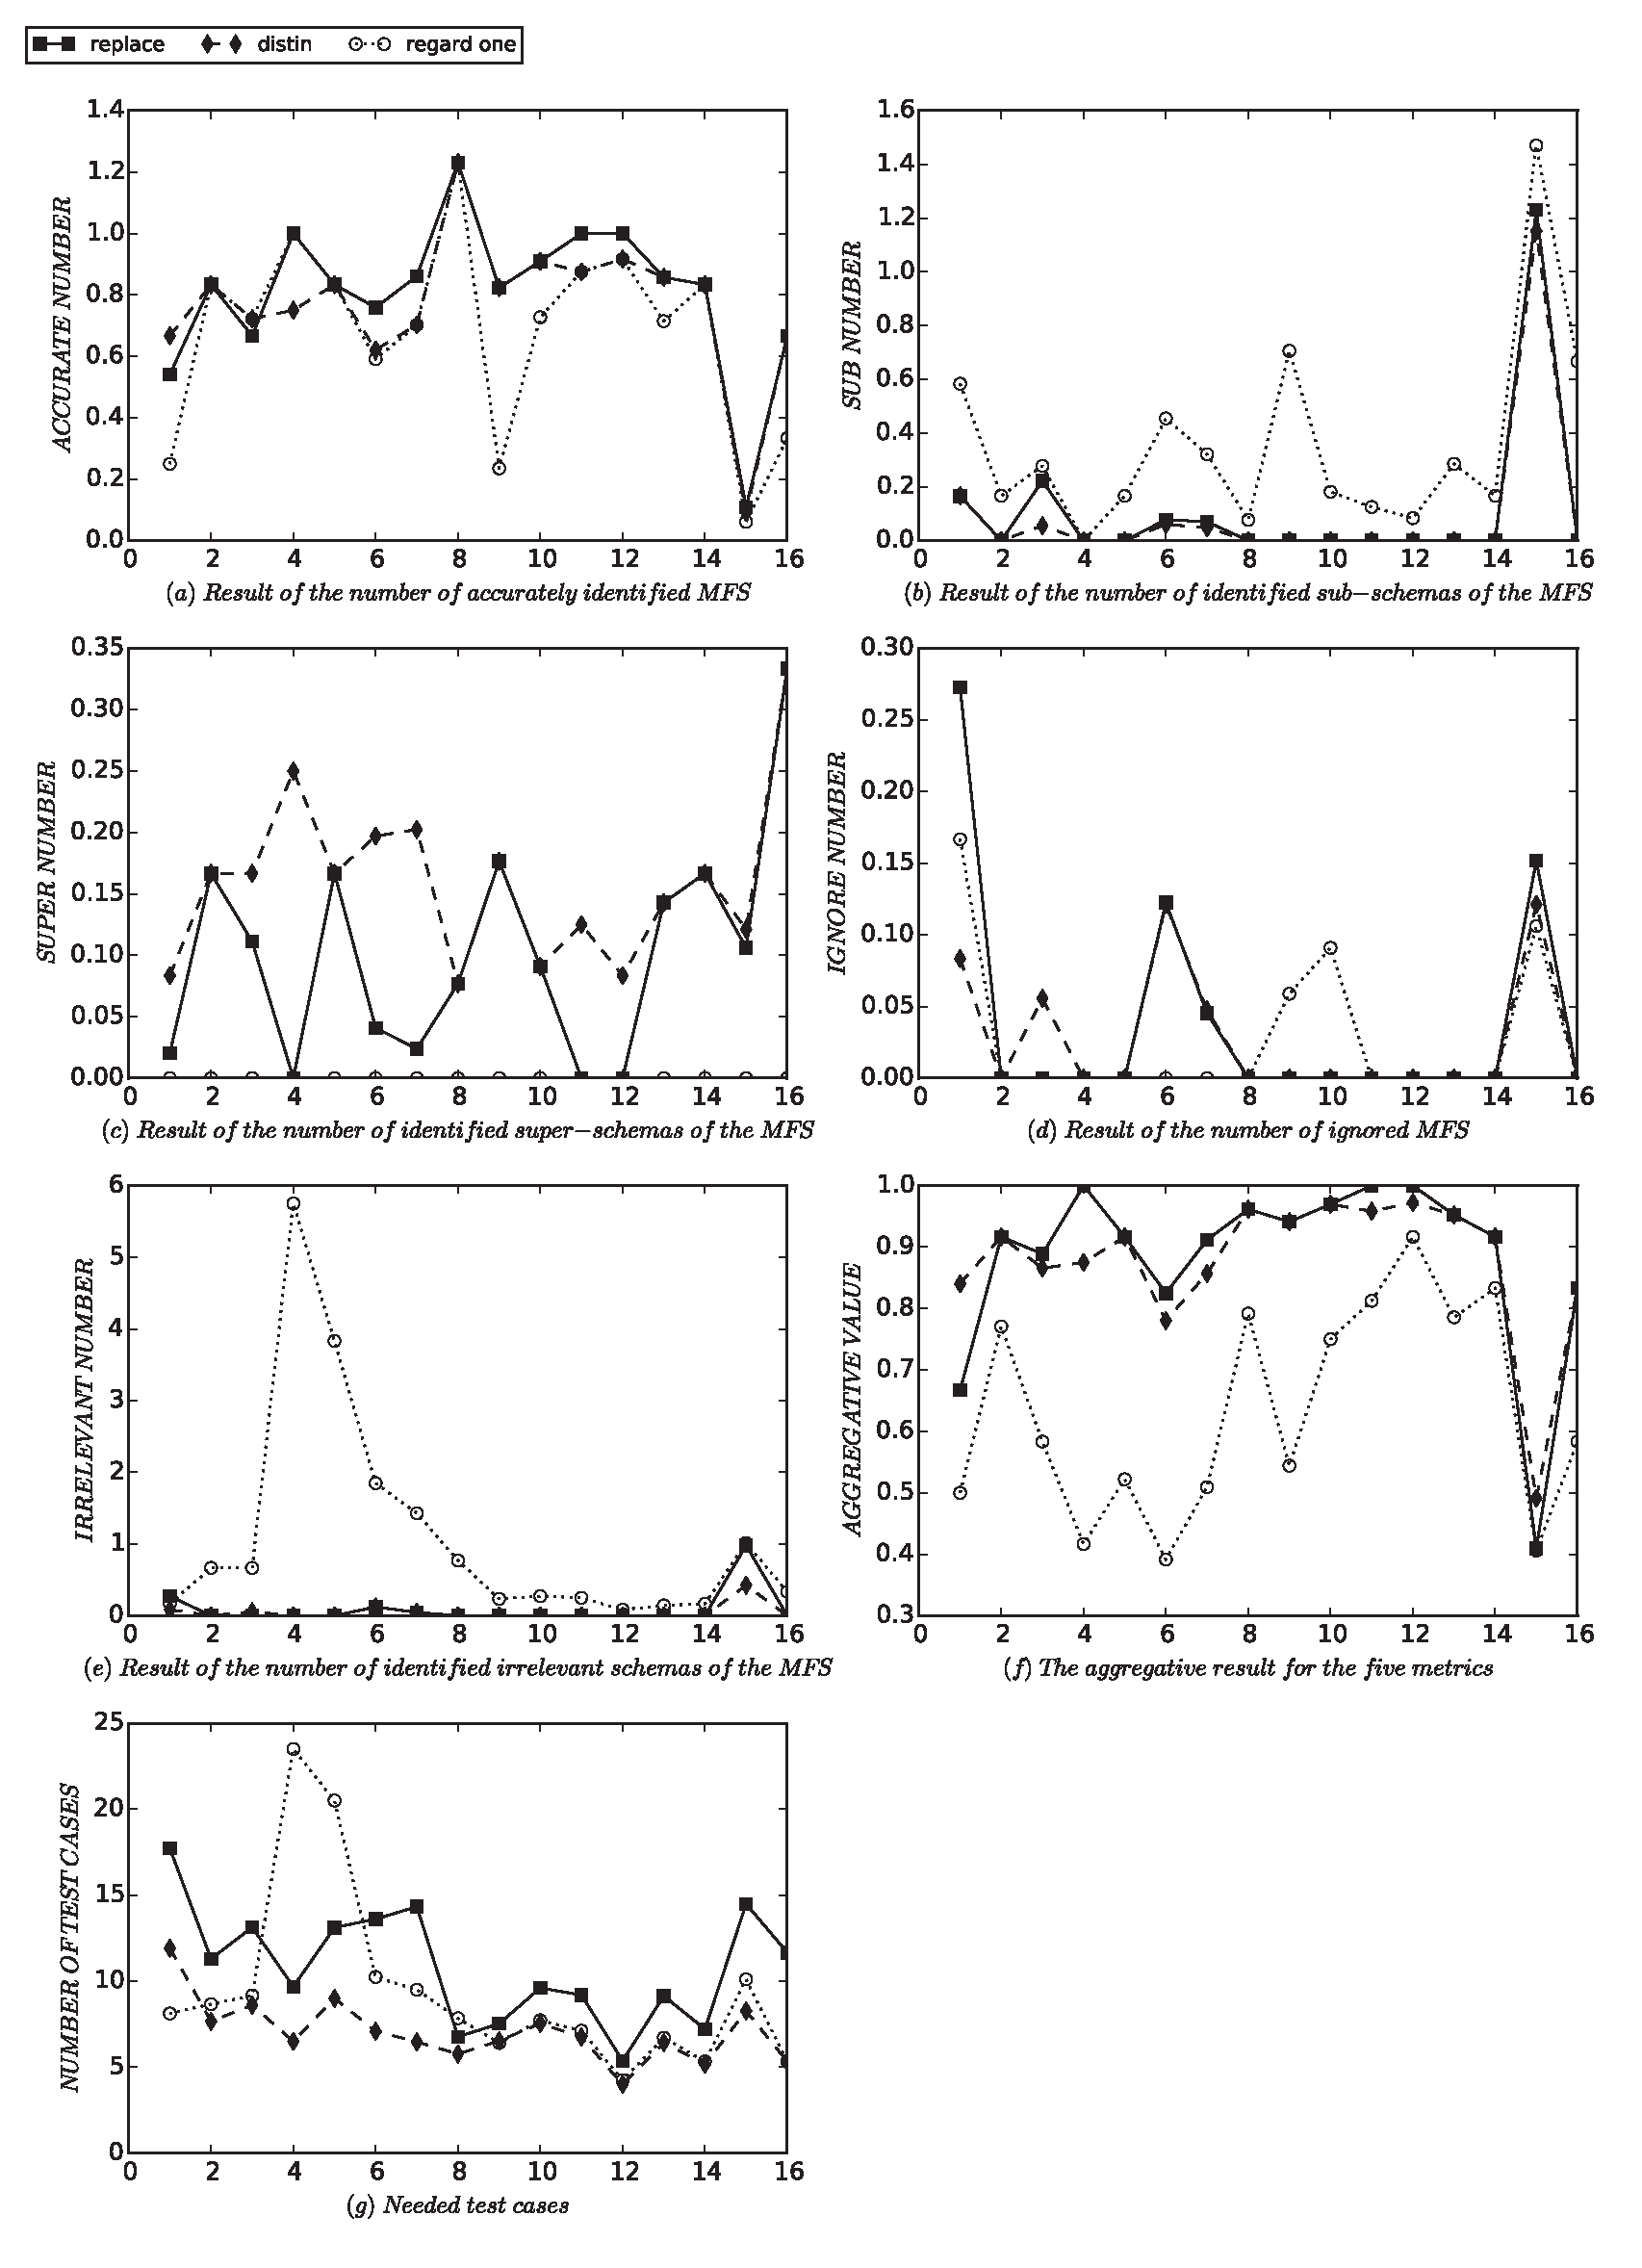
\includegraphics[width=5.60in]{study2.eps}
\caption[Optional caption for list of figures]{Result of the evaluation for the second case study}
\label{fig:comparetotraditional}
\end{figure*}


% Table generated by Excel2LaTeX from sheet 'Sheet1'

Figure \ref{fig:comparetotraditional} depicts the results of the second case study. There are seven sub-figures in this figure, i.e., Figure \ref{fig:comparetotraditional}(a) to Figure \ref{fig:comparetotraditional}(g). They indicate the results of the number of accurate MFS each approach identified, the number of identified schemas which are the sub-schema / super-schema of some prior MFS, the number of ignored prior MFS, the number of identified schemas which are irrelevant to all the prior MFS, the aggregate value, and the extra test cases each algorithm needed, respectively.

In each sub-figure, there are four polygonal lines, each of which shows the results for one of the four strategies: \emph{regarded as same failure}, \emph{distinguishing failures},  \emph{replacement strategy based on ILP searching},  \emph{replacement strategy based on random searching} (The last one will be discussed in the next case study). Specifically, each point in the polygonal line indicates the specific result of a particular strategy for the corresponding testing object. For example in Figure \ref{fig:comparetotraditional}(a), the point marked with `$\blacksquare$' at (1,0.25) indicates that the approach using \emph{regarded as same failure} strategy identified 0.25 accurate MFS on average for each failing test case of the testing object--HSQLDB 2cr8. The raw data for this experiment can be found in Table \ref{evaluation_all} of the Appendix. Note that all these data are average values, i.e., the average performance of these approaches when identifying the MFS for each failing test case.


\textbf{Accurate number: }
Figure \ref{fig:comparetotraditional}(a) shows the average number of accurate schemas that each approach achieved.  It appears that \emph{ILP} performed the best among the three approaches. In fact, for most testing objects (testing objects 1, 4, 5, 6, 7, 9, 10, 11 and 12),  \emph{ILP}  either obtained the most number of accurate MFS, or tie with the most number of accurate MFS.  The second best approach is \emph{distinguishing failures}, which obtained better results than  \emph{regarded as same failure} for testing objects 1, 6, 8, 9, 10, 11, and 12.
% We believe the reason why

%This result shows that our approach can offer the best information for MFS idenr when as it identified the most accurate MFS. For approach .

%We can further find that strategies \emph{replacement strategy based on ILP searching} (short for \emph{ILP}
%later) and \emph{distinguishing failures} have similar results. This can be easily understood, as strategy \emph{ILP} is actually a refinement version of the strategy \emph{distinguishing failures}, which also make the failures distinguished from each other. The main difference between \emph{ILP} and \emph{distinguishing failures} is that the former has to replace the test cases that triggered any failure other than the currently analysed one while the latter will not change the generated test cases. As a result, the comparison of other metrics ( sub, super, ignore, irrelevant numbers) also showed the similarity between strategy \emph{ILP} and \emph{distinguishing failures}.

\textbf{Sub number \& super number: }
Figure \ref{fig:comparetotraditional}(b) and \ref{fig:comparetotraditional}(c) depict the results for \emph{sub number} and \emph{super number}, respectively. These two figures firstly showed a clear trend for strategies \emph{regarded as same failure} and \emph{distinguishing failures}, i.e., the former identified more sub schemas of actual MFS than the latter, while the latter identified more super schemas of actual MFS than the former. This is consistent with our formal analysis in Section \ref{sec:mask:ro} and Section \ref{sec:mask:df}.

%there are 6 scenarios (scenarios 3, 5, 6, 7, 8, 9 listed in Table \ref{conditions-for-ro}) for  strategy \emph{regarded as same failure} that can lead to the identified schemas being sub schemas of actual MFS, while \emph{distinguishing failures} strategy has 2 such scenarios (scenarios 3, 7  in Table \ref{conditions-for-df}). But for the scenarios that can result in the schemas being super schemas of actual MFS, strategy \emph{regarded as same failure} only has one (scenario 2 in Table \ref{conditions-for-ro}), while \emph{distinguishing failure} has 5 such scenarios (scenarios 2, 5, 6,7, 8 in Table \ref{conditions-for-df}).
The performance of our strategy \emph{ILP} for these two metrics are in between. Specifically, ILP identify more sub schemas  than strategy \emph{distinguishing failures} but fewer than \emph{regarded as same failure}; and ILP identify more super schemas than \emph{regarded as same failure}, but fewer than \emph{distinguishing failures}.

  %testing objects 3, 4,7,9,10 13 in Figure \ref{fig:comparetotraditional}(c)). We believe this is an improvement, because too many sub or super schemas in fact point to the same actual MFS, which results in duplication and makes it hard to identify the actual MFS.


\textbf{Ignore number \& irrelevant number: }
The results of the two negative performance metrics are given in Figure \ref{fig:comparetotraditional}(d) and \ref{fig:comparetotraditional}(e), respectively. One observation is that, comparing with strategy \emph{regarded as same failure},  \emph{distinguishing failures} obtained fewer irrelevant schemas, but ignored more actual MFS. This is also consistent with the formal analysis in Section \ref{sec:mask}. Note that for metric \emph{irrelevant number}, strategy \emph{regarded as same failure} obtained significantly much more irrelevant schemas than the remaining strategies, which make it hard to distinguish each other if we post them together on one figure. Hence, we draw this figure with only three polygonal lines (for \emph{distinguishing failures}, \emph{ILP} , and \emph{random} respectively). Besides this, we offer an additional smaller  figure in Figure \ref{fig:comparetotraditional}(e), which includes the strategy \emph{regarded as same failure}, to depicts the comparison of all these approaches.
%***************************************
% if not well, add the fact, particularly that distingusih most no irrelevant shcemas, (objects), indicating that a good control for giving useless information of MFS
%****************************************

%because in our formal analysis the strategy \emph{regarded as same failure} has more scenarios than \emph{distinguishing failures} that can lead to the schemas being irrelevant to the actual MFS,
% in detail, the former has 4 such scenarios (scenarios 4, 6, 8, 9 in Table \ref{conditions-for-ro} ) while the latter has three (scenarios 4, 7,8 in Table \ref{conditions-for-df}).  And for strategy \emph{distinguishing failures}, five scenarios (scenarios 3,6,8,9,10) in Table \ref{conditions-for-df-ignore} increases the chance to ignore the actual MFS than the strategy \emph{regarded as same failure} (scenarios 5, 7 in Table \ref{conditions-for-ro-ignore} ).

The second observation is that \emph{ILP} did a good job at reducing the scores for these two negative metrics. Specifically, for \emph{ignored number}, our approach performed better than strategy \emph{distinguishing failures} for testing objects (1, 3, 7, 10, 11, 12) in Figure \ref{fig:comparetotraditional}(d), but is not as good as strategy \emph{regarded as same failure}. In fact, strategy \emph{regarded as same failure} has a significant advantage at reducing the number of ignored MFS as it tends to associate the failures with all the failing test cases. However, when we consider the \emph{irrelevant number}, our approach is the best among all three strategies ( better than \emph{distinguishing failures} at testing objects 1, 3, 6, 7, 11, 12 in Figure \ref{fig:comparetotraditional}(e), and better than strategy \emph{regarded as same failure} for  almost all the testing objects) . We believe this improvement is caused by our test cases replacing strategy, as it can increase the test cases that are useful for identifying the MFS and decrease those useless test cases.


\textbf{Aggregative for the five metrics: }
The composite results are given in Figure \ref{fig:comparetotraditional}(f). This metric gives an overall evaluation of the quality of the identified schemas. From this figure, we can find that \emph{ILP} performed the best, next the \emph{distinguishing failures}, the last is the \emph{regarded as same failure} (See the testing objects 1, 3, 4, 6, 7, 10, 11, and 12 in Figure \ref{fig:comparetotraditional}(f)).

It is as expected  that \emph{ILP} performed better than \emph{distinguishing failures} as it is actually the refinement version of latter. In fact, \emph{ILP} also make the failures distinguished from each other. The main difference between \emph{ILP} and \emph{distinguishing failures} strategy is that the former has to replace the test cases that triggered any failure other than the currently analysed one while the latter will not change the generated test cases.

It is a bit of surprise to find, however, that strategy \emph{distinguishing failures} performed better than \emph{regarded as same failure} at almost all the testing objects. This result cannot be derived from the formal analysis. We believe the reason is that the masking effects are \emph{monotonic} in the testing objects we constructed for evaluation. That is, our study includes only the case that bug \emph{A} always mask bug \emph{B}, and does not consider cases that bug \emph{A} can mask bug \emph{B} and  bug \emph{B} can also mask bug \emph{A}. This condition is favorable for the \emph{distinguishing failures} strategy. For example, assume bug \emph{A} masks bug \emph{B}; then when we identify the MFS of bug \emph{A}, the \emph{distinguishing failures} is the correct strategy, as if there is a test case trigger the bug \emph{B}, then it must not trigger the bug \emph{A} (otherwise, bug \emph{B} will not be triggered). Hence, the probability that \emph{distinguishing failures strategy} makes the correct operation is at least 50\% .

\textbf{Test cases: }
The number of test cases generated for identifying the MFS indicates the cost of FII approach. The result is shown in Figure \ref{fig:comparetotraditional}(g).  We can find that strategy \emph{ILP} generated more test cases than the other strategies. Specifically, the gap between \emph{ILP} and the other two strategies ranged from about 2 to 5. This is acceptable when comparing to all the test cases that each approach needed. The increase in test cases for our approach is necessary, as additional test cases must be generated when some test cases cannot help to identify the MFS of the currently analysed failure.  As for strategies \emph{distinguishing failures} and \emph{regarded as same failure}, there is no significant difference between them.


Above all, we draw three conclusions, which help to answer \textbf{Q2}:

1)  \emph{Distinguishing failures} strategy obtained more \emph{super number} and \emph{ignored number} than \emph{regarded as same failure} strategy, while the latter identified more \emph{sub number} and \emph{irrelevant number} than the former.  This result is consistent with the previous formal analysis in Section \ref{sec:mask}.

2) Considering the quality of the MFS each approach identified, we can find that our \emph{ILP} approach achieves the best performance, followed by the strategy \emph{distinguishing failures}.

3) Although our approach need more test cases than the other two strategies, it is acceptable.

 %the answer we got for \textbf{Q2} is that: our approach achieves better performance than two traditional strategies when handling masking effects at an acceptable % extra cost.

\subsection{Evaluating the ILP-based test case searching method}\label{sec:emprical:cmILP}
%***************************************
% gives the data for the replacing times and replacing numbers
%****************************************
The third empirical study aims to evaluate the efficiency of the ILP-based test case searching component of our approach. To conduct this study, we implemented an additional FII approach that is augmented by the \emph{replacing test cases} strategy with test case randomly replaced.

%observe the performance of our approach and compare it with the result got by the traditional approaches. Our approach augments the three traditional FII approaches with replacing test cases strategy described in Section 4.
%, and then we applied these augmented approaches to identify the failure-inducing combinations in the prepared subjects.

\subsubsection{Study setup}\label{sec:emprical:cmILP:set}
The setup of this case study is based on the second case study, and uses the same SUT model as shown in Table \ref{testing_models}. We applied the new random searching based FII approach to identify the MFS in the prepared SUTs. To avoid the bias coming from the randomness, we repeated the new approach 30 times to identify the MFS in each failing test case. We then computed the average additional test cases as well as other metrics listed in section \ref{sec:emprical:cmtradition:set} for the random-based approach. As the approach involves the random replacement, we conducted t-test on the original 30 groups of data to test the difference between the random-based approach and the ILP-based approach.

% We will also take a look at how many scores can the new approach get when measuring the aforementioned metrics, as the same, we just compare the average scores with traditional ones.
%Additionally, comparisons between the augmented approaches and three traditional ones will be quantified.

\subsubsection{Results and discussion}\label{sec:emprical:cmILP:rs}
The evaluation of this random-based approach is also shown in Figure \ref{fig:comparetotraditional}, in which the polygonal line marked with  `$\star$' indicates the results. The raw data can also be found in the Row `R' of Table \ref{evaluation_all} in the appendix. It is noted that for the random approach we just give the average result of 30 tries.  We offer the p-value in the Row `P(I,R)' of Table \ref{evaluation_all}. Note that A p-value smaller than 0.05 indicates that the performance of these two approaches are statistically different with each other at 95\% confidence.

Compared to the ILP-based approach, we can firstly observe that there is little distinction between them in terms of the metrics super-schemas and sub-schemas. For metric accurate number, the ILP-based approach performs slightly better (see testing objects 1, 6, 7, 11, where ILP obtained more accurate MFS), and for metrics ignore and irrelevant number, the ILP-based approach also has a slightly better performance, i.e., ILP obtained smaller number of these schemas which are of no-use for testing. Combining these results, we conclude that the ILP-based approach has a similar performance as random-based approach at the quality of identified MFS (The former may perform slightly better at some testing objects). This is consistent to Figure \ref{fig:comparetotraditional}(f).

The similar quality of MFS identification of these two approaches can also be embodied with the p-values we obtained. From Table \ref{evaluation_all} in the Appendix, we can learn that, for all these metrics except for `testNum'( which will be discussed later), there exists some p-values that are \emph{NaN} (Not a number). This is because for these testing objects, the results are the same for all the 30 tries. The reason that the results are the same is because the only random part of the approach is the test case replacement. This random process normally does not affect the determination of whether a schema is failure-inducing or not, as no matter which test case we choose, the replacement has the same ending condition, i.e., to find some test case that triggers the same failure or pass (The only exception is that different test cases for replacement may introduce some newly MFS of the same failure, which will interfere with the MFS identification process \cite{zhang2011characterizing} ). As a result, the MFS identified will be the same for the 30 tries for most cases.  Then as the random part normally does not affect the quality of the MFS identification, it is conceivable that these two approaches have a similar performance as they both use the \emph{test case replacement} strategy.

%even if we repeated 30 times, the basic strategy is to replace a test case . For most cases, it will not, but for two the approach will not accurate, this is becasue safe value is not satisfied. As


\begin{figure}[htbp]
\centering
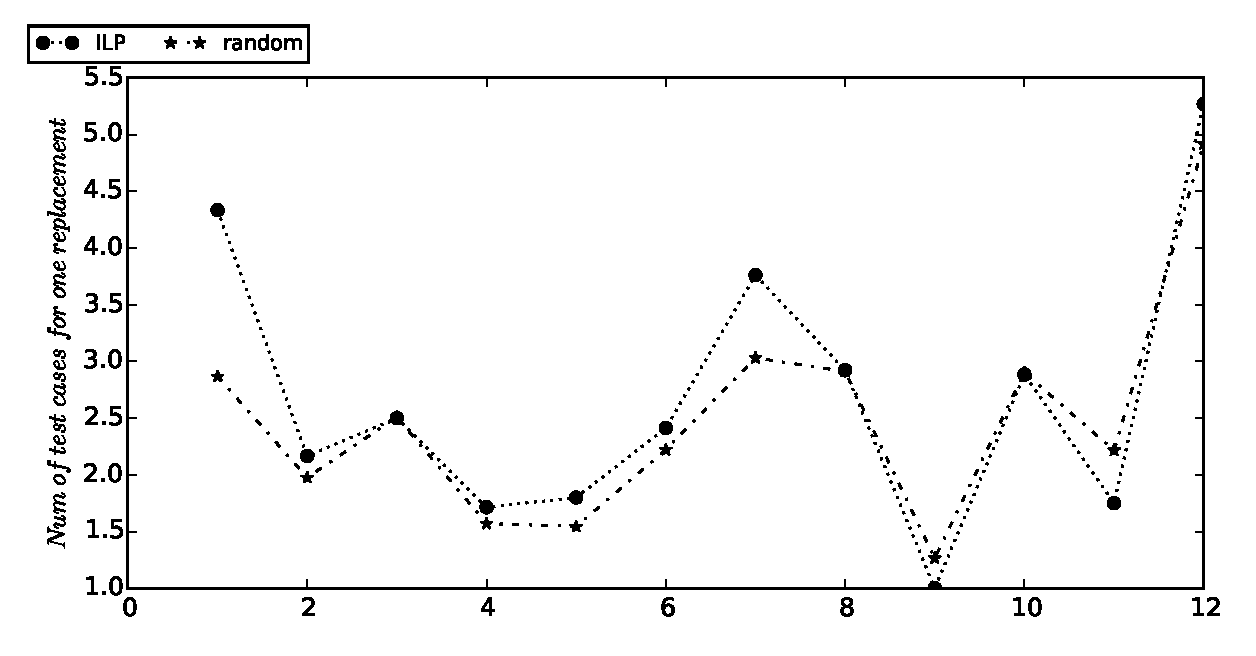
\includegraphics[width=4.10in]{replacingtimes.eps}
\caption{The comparison of the number of replacement test cases}
\label{fig:replacing}
\end{figure}


Secondly, when considering the cost, we find that the ILP-based approach performs better. In fact, for each failing test case, it can reduce on average 1 to 2 test cases (about 7.1\% to 14.2\% of the overall number of test cases needed for MFS identification) when compared to the random-based procedure (See testing objects of Figure \ref{fig:comparetotraditional}(g)). This reduction is impressive, as when considering the total number of failing test cases for one software (See Table \ref{masking effect condition}), it can reduce thousands of test cases in total when conducting MFS identification on each software.
This conclusion is statistically significant, as we can learn that the p-value of these two approaches for this metric is extremely small, which ranged from 1.74E-26 to 1.26E-71 (See Row `testNum' of Table \ref{evaluation_all} in the Appendix).


To be precise, we next compared the test cases only used for replacement of the two approaches. By this we can eliminate the interference of other test cases for identifying MFS, and focus on the performance of the key part of these two approaches --- the replacement strategy. Figure \ref{fig:replacing} shows the result. We can learn that on average,  for each call of the replacement algorithm, ILP can save about 1 test case. Note that this reduction is not trial when considering the overall number of test cases for MFS identification.  We listed the original data and p-values in Table \ref{replacementavg}. It can be easily learned that the difference between these two approaches is also statistically significant, as the Row `$\mathcal{P}$' shows all p-values are very small.

\begin{table}\renewcommand{\arraystretch}{1.3}
\tbl{The average test cases needed for one replacement\label{replacementavg}}{
\setlength\tabcolsep{1.3pt}
\begin{tabular}{|l|llllllllllll|}
\hline
&H2cr8 & H2.2.5 & H2.2.9 & J1.4.1 & J1.4.2 & G2.6.3 & G2.22 & syn1     & syn2     & syn3     & syn4     & syn5               \\ \hline
ILP      & 1         & 1         & 1.77       & 1.75       & 1.66      & 2.34     & 1.73     & 2.24     & 0.16     & 3.3      & 1.04     & 2.81     \\
Rand   & 2.11      & 1.66      & 2.22       & 2.5        & 2.66      & 3.37     & 2.64     & 2.29     & 0.24     & 3.38     & 1.54     & 2.85     \\
$\mathcal{P}$  & 1.6E-60  & 1.1E-51  & 1.3E-51   & 2.5E-67   & 3.9E-70  & 8.0E-37 & 1.5E-42 & 2.5E-28 & 2.1E-28 & 1.1E-28 & 4.3E-45 & 3.2E-16 \\ \hline
\end{tabular}
}
\end{table}


In summary, the answer for \textbf{Q3} is that searching for a satisfied test case affects the performance of our approach, especially regarding the number of extra test cases, and the ILP-based approach can handle the masking effects at a relatively smaller cost than the random-based approach.

%\subsection{Voting System}
%The last empirical study aims to observe the performance of our approach and compare it with the result got by the traditional approaches. Our approach augments the three traditional FII approaches with replacing test cases strategy described in Section 4.
%%, and then we applied these augmented approaches to identify the failure-inducing combinations in the prepared subjects.
%
%\subsubsection{Study setup}
%The setup of this case study is almost the same as the second case study. The difference is that the algorithms we choose are three augmented ones.
%
%%Additionally, comparisons between the augmented approaches and three traditional ones will be quantified.
%
%\subsubsection{Result and discussion}
\subsection{Comparison with Feedback driven combinatorial testing}\label{sec:emprical:cmFD}
The \emph{FDA-CIT} \cite{yilmaz2013reducing} approach handle masking effects by generating covering array that can cover all the $\tau$-degree schemas without being masked by the MFS. There is an integrated FII approach in the FDA-CIT, which has two versions, i.e., \emph{ternary-class} and \emph{multiple-class}. In this paper, we use the multiple-class version for comparison, as it performs better than the former \cite{yilmaz2013reducing}.   %, the configuration options for J48, is .


The FDA-CIT process starts with generating a covering array (In \cite{yilmaz2013reducing}, this is a test case-aware covering array \cite{yilmaz2013test}). After executing the test cases in this covering array, it records the outcome of each test case and then applies the classification tree method on the test cases to characterize the MFS of each fault. It then labels these MFS as the schemas that can trigger masking effects. Later, if the interaction coverage is not satisfied (here the interaction coverage criteria is different from the traditional covering array \cite{yilmaz2013reducing}), it will re-generate a covering array that aims to cover these schemas that were masked by the MFS and then repeat the previous steps.

The main target of FDA-CIT is to guarantee that the generated test cases should cover all the $\tau$-degree schemas. To achieve this goal, FDA-CIT needs to repeatedly identify the schemas that can trigger the masking effects. So to make the two approaches (FDA-CIT and ILP) comparable, we need to collect all the MFS that FDA-CIT characterized in each iteration and then compare them with the MFS identified by our approach.

\subsubsection{Study setup}\label{sec:emprical:cmFD:set}

As FDA-CIT used a post-analysis (classification tree) technique on covering arrays, we first generated 2 to 4 ways covering arrays. The covering array generating method is based on augmented simulated annealing \cite{cohen2003augmenting}, as it can be easily extended with constraint dealing and seed injection \cite{cohen2007interaction}, which is needed by the FDA-CIT process. As different test cases will influence the results of the characterization process, we generated 30 different 2 to 4 way initial covering arrays. Then before we feed them to the FDA-CIT approach, we extend the corresponding $\tau$-way covering array to $\tau$+1-way covering array. This is because FDA-CIT needs higher-way covering arrays to identify MFS \cite{yilmaz2013reducing}. The classification tree method which is integrated into FDA-CIT is implemented by Weka J48 \cite{hall2009weka}, of which the configuration options are set as follows:  the \emph{n}-fold of cross validation is set to 10, the accuracy cutoff is set to be 1 and the default confidence factor is 0.25 \cite{yilmaz2006covering}.  After running FDA-CIT, we recorded the MFS identified, and by comparing them with prior actual MFS, we can evaluate the quality of the identified schemas according to the metrics mentioned in the previous case study.

%which consists of the metrics mentioned in the second case study.

Besides the FDA-CIT, we also applied our ILP-based approach to the initial $\tau$-way covering array. Specifically, for each failing test case (except those test cases which contain existed identified MFS) in the covering array, we separately applied our approach to identify the MFS of that case. In fact, we can reduce the number of extra test cases if we utilize the other test cases in the covering array \cite{li2012improved}), but we did not utilize the information to simplify the experiment. Similarly, we then recorded the MFS identified by our approach, and evaluated them according to the corresponding metrics. In addition, we recorded the overall test cases (including the initially generated covering array) that this approach needed and compared the magnitude of these test cases with that of FDA-CIT.

%
% We then merged all the test cases that our approach needed for each failing test case in the covering array, and we also merged other metrics listed in the second case study for each failing test case.


%As mentioned before, the FII approach in FDA-CIT, i.e., classification tree algorithm, is a post-analysis technique. Given different test sets, the results identified by the classification tree algorithm are also different. Then a natural question is, what the schemas identified by FDA-CIT will be if the classification tree method is applied on the test cases generated by our ILP approach? This question is of importance as first, we can learn whether the test cases generated by ILP can help FDA-CIT approach to improve the quality of the identified schemas; second, the comparison between ILP and FDA-CIT will be more fair as they share the same test cases. For this, a new approach that is based on FDA-CIT is introduced, which is augmented by replacing the original test cases in FDA-CIT with those generated by ILP approach. Then the schemas identified by the classification tree algorithm in FDA-CIT are recorded and evaluated. This new approach is referred to as \emph{FDA-CITs} later.

\subsubsection{Result and discussion}\label{sec:emprical:cmFD:rs}

The result is shown in Figure \ref{fig:comparefda}. There are three sub-figures of Figure \ref{fig:comparefda}, which describe the results of the experiments based on 2-way, 3-way and 4-way covering arrays, respectively.  In each sub-figure, there are 7 columns, showing the outcomes for the previous mentioned 6 metrics and one more metric (Column \emph{Testcase}), which indicates the overall test cases that each approach needed. Each column has two bars, which indicate the results for approach FDA-CIT, and ILP respectively.

Note that in Figure \ref{fig:comparefda}, the results for each metric is the average evaluation for all the results of the experiments on the 12 testing objects in Table \ref{testing_models}. The raw results (as well as the p-values) for each testing object are listed in Table \ref{comparewithfda} in the appendix. The raw data is organised the same way as Table \ref{evaluation_all}.


 \begin{figure*}[htbp]
\centering
\subfigure[Result for the 2-way covering array]{
  %  \rule{4cm}{3cm}
    \label{fig:31}
    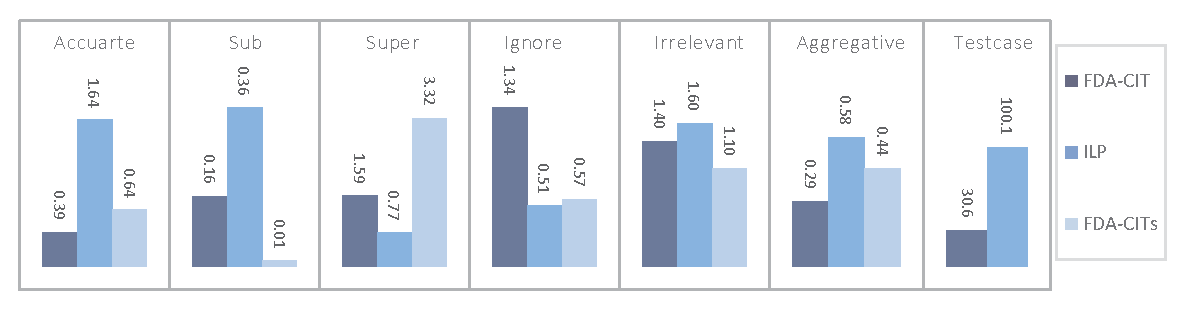
\includegraphics[width=4.4in]{2-way.eps}
}
\subfigure[Result for the 3-way covering array]{
  %  \rule{4cm}{3cm}
    \label{fig:32}
    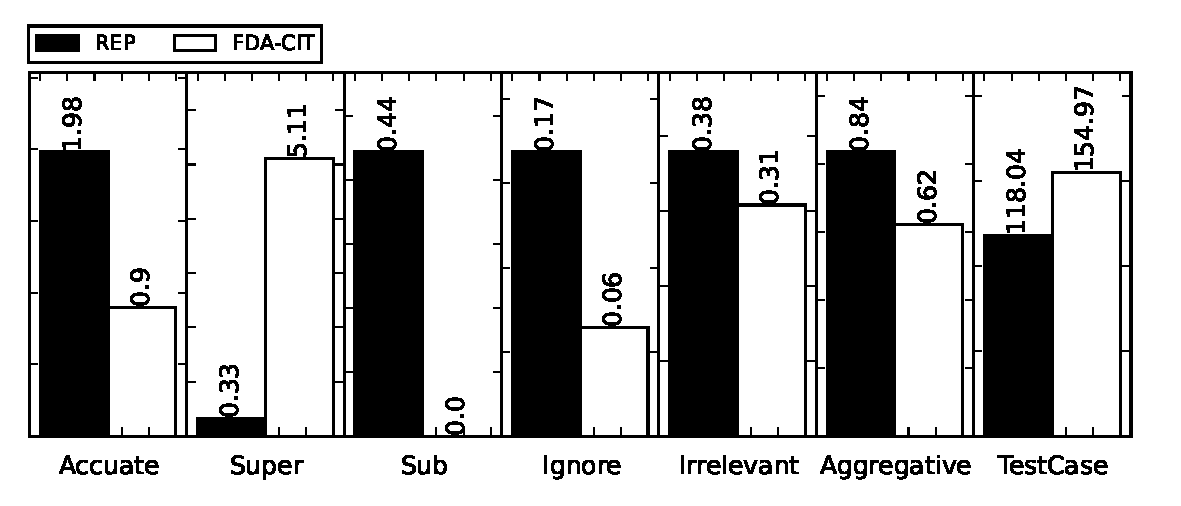
\includegraphics[width=4.4in]{3-way.eps}
}
\subfigure[Result of the 4-way covering array]{
  %  \rule{4cm}{3cm}
    \label{fig:33}
    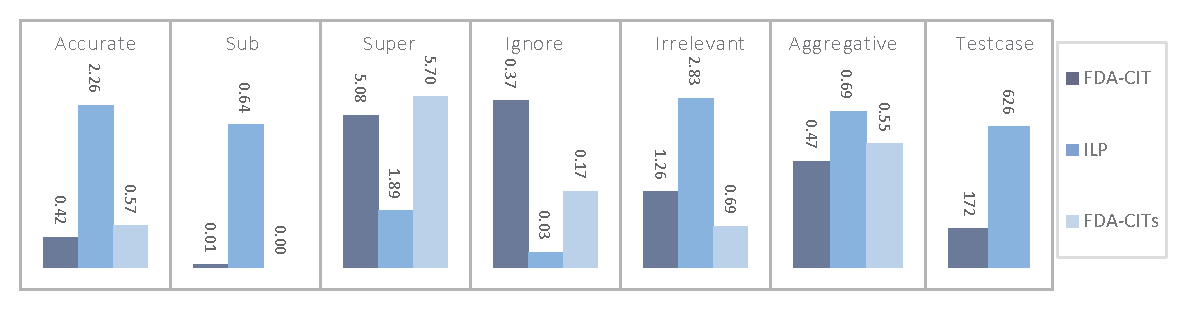
\includegraphics[width=4.4in]{4-way.eps}
}
\caption[Optional caption for list of figures]{Three approaches augmented with the replacing strategy}
\label{fig:comparefda}
\end{figure*}


From Figure \ref{fig:comparefda}, we have the following observations:

First, for most metrics in our study, the performance of each approach is relatively stable against the change of degree $\tau$. The only exceptions are metrics \emph{ignore number} and \emph{irrelevant number}. With increasing $\tau$, the value of ignore number and irrelevant number of approach \emph{FDA-CIT} decrease rapidly, while the performance of \emph{ILP} is relatively steady when compared to \emph{FDA-CIT}. Apart from these two metrics, the relationships between the two approaches for the other metrics are stable. Take for example the metric \emph{accurate number}. No matter what $\tau$ is (2, 3 or 4), \emph{ILP} always obtained more accurate schemas than \emph{FDA-CIT}. This observation indicates that the difference between the performance of these approaches is not dependent on the characteristics of the covering array, but instead on the approaches themselves.

From the perspective of p-values, we can also get the same observation. For all the metrics except \emph{ignore number} and \emph{irrelevant number}, the p-values are relatively small. Note that there also exist some test objects that the p-values are \emph{NaN}. This is because that the MFS of these testing objects are relatively simple (between  2 to 3 MFS). As a result, both approaches obtained the same schemas for the 30 tries. Besides the \emph{NaN} values, other values of these metrics indicates that the difference between these two approaches are statistically significant. As for metrics \emph{ignore number} and \emph{irrelevant number}, the p-values are relatively large. For example, for the 2-way experiment, some p-values of metric \emph{ignore} are around 0.3 (Column `\emph{syn1}') and 0.1 (Column `\emph{syn3}'), which show that there are no significant different between the two approaches for this metric.

%Second, with increasing \emph{t},  the overall performance of each approach is improved. For example, the score of the aggregative metric of \emph{ILP} is 0.55, 0.66 and 0.69, respectively, for \emph{t} equals to 2, 3 and 4. The improvement is mainly because with increasing \emph{t}, the number of test cases also increased. Accordingly, the approach will observe more failing test cases,
%%(See area B in Figure \ref{fig:fci_process}),
% so that we can get the schemas more close to the actual MFS.

Second, comparing to \emph{ILP}, the schemas identified by \emph{FDA-CIT} tend to be super schemas rather than sub schemas of the original MFS. We believe this result is due to the use of the classification tree analysis. Note that the way that CTA constructing decision trees usually work top-down, by choosing a parameter value at each step that best splits the set of test cases \cite{rokach2005top}. After that, one path (conjunction of nodes from the root to a leaf in the tree) in this tree is deemed as an MFS. Consequently, the MFS identified by FDA-CIT tends to share some common nodes (here, a node represents a parameter value), e.g. the root node, which result in the identified schemas containing some unnecessary parameter value. This induces the so-called `over fitting' problem. As a result, the schemas identified by \emph{FDA-CIT} tend to be the super schemas of the actual MFS.

%Note that the difference between the number of identified super schemas is statistically significant, as the p-values shown in the Column `super' are very small in Table \ref{comparewithfda} for all the three degrees.

%Other observations include:

%First, compared with the original approach \emph{FDA-CIT}, \emph{FDA-CITs} has obvious advantages at almost all the metrics except for \emph{super number}. In detail, \emph{FDA-CITs} obtained more schemas that are identical to the actual MFS (\emph{accurate number}), fewer schemas that are the sub schemas of actual MFS (\emph{sub number}), and lower scores for the two negative metrics (\emph{ignored number} and \emph{irrelevant number}). At last, the schemas identified by \emph{FDA-CITs} showed an overall higher quality than that of the original \emph{FDA-CIT} (\emph{aggregative metric}).  We have discussed previously that \emph{FDA-CIT} tends to identify super-schemas of actual MFS when the test cases increase. So for metric \emph{super number}, it is no surprise that \emph{FDA-CITs} identified more super schemas of actual MFS than \emph{FDA-CIT}, because it used the test cases generated by \emph{ILP}, which were more than that of the original FDA-CIT. The difference between the overall performance of \emph{FDA-CIT} and \emph{FDA-CITs} is also expected. In fact, this result is consistent with our previous observation that when \emph{t} increases, the overall performance for each approach also increases.

%
%This result indicates that the number of test cases is a key factor that affects the performance of the approach FDA-CIT. And the more test cases are, the better the FDA-CIT will perform, though FDA-CIT would also identified more super schemas of the actual MFS.

Third, in terms of the quality of the MFS identified, we can clearly find that our approach performed better than FDA-CIT. This is manifested in that our approach obtained more accurate schemas (the differences are statistically significant for all 3 degrees). We believe this gap is mainly caused by the FII approach. However, this result does not mean that FIC\_BS is better than the classification tree method under all conditions. In fact, the classification tree method has its own advantage, i.e., it is flexible and does not need to generate additional test cases. As a result, FDA-CIT can be applied to some complex testing scenarios, e.g., occasional failures, and incompatibilities between test cases and configurations \cite{yilmaz2013reducing}.

%and as a result, \emph{FDA-CIT} generated fewer test cases than that of \emph{ILP}.

At last, when considering the cost of these two approaches, our approach needs fewer test cases. However, it should be noted that FDA-CIT is conducted on $\tau$+1 way covering arrays. Hence, FDA-CIT can get better performance when using $\tau$-way covering array.

%It is noted that, these observations are all statistically significant.
%*************************************************************
% The second reason that why our approach generated more test cases than \emph{FDA-CIT} is that .


%for the approaches \emph{FDA-CIT} and \emph{FDA-CITs}, we can find the latter performed better than the former.
%In terms of , we can have the following
%When we fix the degree \emph{t}, we can learn the following with respect to
%
%We firstly
%
%
%Then we .

Above all, we can conclude three points in this experiment, which provide answer to \textbf{Q4}:

%1) FDA serial ����, and the ILP ���ӿ��ţ���˸����ʺϡ�

1)The degree $\tau$ of the covering array does not affect the overall performance of approaches, but for FDA-CIT, it may get better performance at reducing the \emph{ignore number} and \emph{irrelevant number} when using higher-$\tau$-way covering array.

2)When taking account of the quality of MFS identification, \emph{ILP} approach preforms better.

3)Without additional measures, FDA-CIT is a better choice when handling some complex testing scenarios.
%Considering the quality of the MFS each approach identified, \emph{ILP} performed better than the other two approaches, although it needed more test cases.

%Based on these observations, a recommendation for selecting masking handling techniques in practice is that to get a more precise identification of the  MFS in the SUT, \emph{ILP} is preferred, and for lower number of test cases,  \emph{FDA-CIT} may be a better choice.

It is noted that FDA-CIT's primary concern is to avoid masking effects and to give every $\tau$-degree a fair chance to be tested, not to perform fault characterization. FDA-CIT is also an established technique which can work with non-deterministic failures and in the presence of inter-option constraints. So even though our approach \emph{ILP} has shown a better performance at MFS identification, it is appealing and effective to use FDA-CIT to guide the test generation when taking into account the masking effects. In fact, considering FDA-CIT can work with other fault characterization approaches, it may also be appealing to combine these two approaches for MFS identification.

%3)The increasing t a overall improvement for the quality but also increasing the test cases.

%
%From this result, we can first observe that in all the cases our ILP-based approach can more accurately identify the MFS and ignored less MFS than the FDA-CIT approach. For the metric `super-schema', `sub-schema', and `irrelevant schemas', there are ups and downs on both sides. With respect to the `overall metric', we find our approach has a significant advantage over the FDA-CIT, but it also requires many more test cases than FDA-CIT.
%
%We note that, when applying the multiple-class FII to characterize the MFS with the test cases that were generated using our approach, their `overall' metric is still not as good as our ILP-based approach, but may show some improvement over the original FDA-CIT.
%
%Another interesting observation is that overall performance in most cases is increasing with the $t$, which can be easily understood. More test cases will contain more information about the MFS, so that we can utilize them to identify the MFS more precisely.
%
%%
%%the t more, the result is more good, but there must be the over-fit problem, for example, for.
%%
%%it is because the improvement by the t-coverage is increasing quickly when the bug is 2-4 or large than 2, if the bug itself is less than 2 -4 , than the improvement is not obviously.
%
%So the answer for \textbf{Q4} is that: our approach can achieved a more precise result for the MFS, and the FDA-CIT can perform the identifying process using a small amount extra test cases. Both of these two approaches have their ups and downs, choosing which approach in practice will depend on the specific scenario you test.
%% if you want to get a more precise result and more helpful test cases generating supply, you should choose our approach, however if you are limited to the test cases execution, you can choose the feedback driven.
%% but if
\subsection{Threats to validity}\label{sec:threats}

%This section gives the threats to internal validity and external validity of our study.
%\subsubsection{construct threats}
%We use the five metrics to demonstrate the validate the effectiveness of our approach, this is derived from the intuitive point.

\subsubsection{internal threats}\label{sec:threats:internal}
There are two threats to internal validity. First, the characteristics of the actual MFS in the SUT can affect the FII results.  This is because the magnitude and location of the MFS can make the FII approaches generate different test cases. As a result, it can lead to different observed failing test cases and inferred failing test cases. In the worst case, the FII approach happens to identify the exact actual MFS, then our test case replacing strategy is of no use. In this paper, we used 12 testing objects, in which 5 are real software systems with real faults and 10 synthetic ones with injected faults. To reduce the influence caused by different characteristics of the MFS, we need to build more testing objects and inject additional types of faults for a more comprehensive study of our approach.

%
% The identifying approach can affect.
%
%The second threat comes from the input model we built. As we focused on the options related to the perfect combinations and only augmented it with some noise options, there is a chance we will get different results if we choose other noise options. More options needed to be tested to see whether our result is common or just appears in some particular input models.

The second threat is that we just applied our test case replacing strategy on one FII approach -- FIC\_BS \cite{zhang2011characterizing}. Although we believe the test case replacing strategy can also improve the quality of the identified MFS for other FII approaches when the testing object is suffering from masking effects, the extent to which their results can be refined may vary for different FII approaches. For example, for FIC\_BS \cite{zhang2011characterizing} used in this paper, there are about $(v - 1)$ to $(v - 1)^{k - 1}$ ($k$ is the number of parameters in a test case, $v$ is the number of values each parameter can take) candidate test cases that can be replaced when one test case triggered failure of other fault, while for OFOT \cite{nie2011minimal}, there are $(v - 1)$ candidates. As a result, FIC\_BS can have a higher chance than OFOT to find a satisfied test case.  To learn the difference between the improvement of various FII approaches when applying our test case replacing strategy, we need to try more FII approaches in the future.

% And  so further works needed to examine more algorithms in this field to obtain a more general result.

\subsubsection{external threats}\label{sec:threats:external}

One threat to external validity comes from the real software we used.  In this paper we have only surveyed two types of open-source software with five different versions, of which the program scale is medium-sized. This may impact the generality of our results.
% Although we believe it is quite possibly a common phenomenon in most software that contains multiple faults which can mask each other, we need to investigate more software to support our belief.



%alleviate the impact of multiple faults is to take a trial-and-error process, i.e., initially classify failures by random and then identify the MFS and fix the bugs based on the classification, after which if the program still doesn't work, then the classification process will be refined and the previous steps continue.

The second threat comes from the possible masking relationships between multiple faults in the real software.  In this paper, we just focus on the condition that the masking effects are transitive, i.e., if fault \emph{A} masks \emph{B}, and fault \emph{B} masks \emph{C}, then fault \emph{A} must mask fault \emph{C}. In practice, the relationships between multiple faults may be more complicated. One possible scenario is that two faults are in a loop, for which they can even mask each other in a particular condition. Such a case will make our formal analysis invalid and will significantly complicate the relationships between schemas and their corresponding test cases. A new formal model should be proposed to handle that type of masking effects.

The third threat is that all the failures in the experiments are option-related. In practice, some failures may not be related to the parameters modeled in the SUT. For example, consider the Internet Explorer option-compliant testing problem \cite{nie2013adaptive}. Initially we may not properly model the options we tested, as a result, it can happen that the explorer will always crash no matter we change which option in the initial model. This will cause the MFS identification invalid, as all the test cases fail during testing. To solve this problem, one potential solution is to re-model the options we should test, as the error may be related to other options in the SUT (For example, those options which are set to default value). Or alternately, we should try other testing techniques to assist original CT. For example, if the error is related to the internal code instead of those configuration options, we may try program slicing technique \cite{weiser1981program} or spectrum-based approaches \cite{naish2011model}. In such case, the parameters that we model for the SUT should not only be limited to configuration options or simple inputs, but also those variables, predicates, or other logical structures and data in the software under test.

%
% not the directly linear about multiple faults, i.e., failure a can mask the failure b, failure b can mask a . and failure c can mask failure c. Even worse, two failures can mask each other. When such scenorias happened, we need to recoonsruct the formal model of the schemas that when can be either be.  as the condition will significantly completed the relationships between the failures and schemas. But anyhow, our appraohc can still work in such a way, as the will always good to identify the MFS.

\section{related works}\label{sec:related}

Shi and Nie \cite{shi2005software} presented an approach for failure revealing and failure diagnosis in CT , which first tests the SUT with a covering array, then reduces the value schemas contained in the failing test case by eliminating those appearing in the passing test cases. If the failure-causing schema is found in the reduced schema set, failure diagnosis is completed with the identification of the specific input values which caused the failure; otherwise, a further test suite based on SOFOT is developed for each failing test case, and the schema set is then further reduced, until no more faults are found or the fault is located. Based on this work, Wang \cite{wang2010adaptive} proposed an AIFL approach which extended the SOFOT process by adaptively mutating factors in the original failing test cases in each iteration to characterize failure-inducing interactions.

Nie et al. \cite{nie2011minimal} introduced the notion of Minimal Failure-causing Schema(MFS) and proposed the OFOT approach which is an extension of SOFOT that can isolate the MFS in the SUT. This approach mutates one value of that parameter at a time, hence generating a group of additional test cases each time to be executed. Compared with SOFOT, this approach  strengthens the validation of the factor under analysis and can also detect the newly imported faulty interactions.

Delta debugging \cite{zeller2002simplifying} is an adaptive divide-and-conquer approach to locate interaction failure. It is very efficient and has been applied to real software environment. Zhang et al. \cite{zhang2011characterizing} also proposed a similar approach that can efficiently identify the failure-inducing interactions that have no overlapped part. Later, Li \cite{li2012improved} improved the delta-debugging based approach by exploiting useful information in the executed covering array.

Colbourn and McClary \cite{colbourn2008locating} proposed a non-adaptive method. Their approach extends a covering array to the locating array to detect and locate interaction failures. Mart{\'\i}nez \cite{martinez2008algorithms,martinez2009locating} proposed two adaptive algorithms. The first one requires safe value as the assumption and the second one removes this assumption when the number of values of each parameter is equal to 2. Their algorithms focus on identifying faulty tuples that have no more than 2 parameters.

Ghandehari et al. \cite{ghandehari2012identifying} defined the suspiciousness of tuple and suspiciousness of the environment of a tuple. Based on this, they ranked the possible tuples and generated the test configurations. They \cite{ghandehari2013fault} further utilized the test cases generated from the inducing interaction to locate the fault.

Yilmaz \cite{yilmaz2006covering} proposed a machine learning method to identify inducing interactions from a combinatorial testing set. They constructed a classification tree to analyze the covering arrays and detect potential faulty interactions. Beside this, Fouch{\'e} \cite{fouche2009incremental} and Shakya \cite{shakya2012isolating} made some improvements in identifying failure-inducing interactions based on Yilmaz's work.

Our previous work \cite{niu2013identifying} proposed an approach that utilizes the tuple relationship tree to isolate the failure-inducing interactions in a failing test case. One novelty of this approach is that it can identify the overlapped faulty interaction. This work also alleviates the problem of introducing new failure-inducing interactions in additional test cases.

In addition to the studies that aim at identifying the failure-inducing interactions in test cases, there are others that focus on working around the masking effects.

Constraints handling becomes more and more popular in CT these years. A constraint is an invalid interaction that should not appear in the test case. It can be deemed as the masking effect which are known in prior \cite{yilmaz2013reducing}.  Cohen \cite{cohen2007exploiting,cohen2007interaction,cohen2008constructing} studied the impact of the constraints that render some generated test cases invalid in CT. They also proposed an approach that integrates the incremental SAT solver with the covering arrays generating algorithm to avoid those invalid interactions. Further study was conducted \cite{petke2013efficiency} to show that with consideration of constraints, higher-strength covering arrays with early failure detection are practical.

Besides, there are additional works that aim to study the impact of constraints for CT \cite{garvin2011evaluating,bryce2006prioritized,calvagna2008logic,grindal2006handling,yilmaz2013test}.
Among them, \cite{bryce2006prioritized} distinguished the constraints into two types: \emph{hard} and \emph{soft}, which the former cannot be included in the test case, while the latter can be permitted, but not desirable.  \cite{grindal2006handling} comprehensively compared the performance of four strategies at handling the constraints in the covering array. \cite{calvagna2008logic} proposed an heuristic strategy to handle the constraints. It can support an ad-hoc inclusion or exclusion of interactions such that the user can customize output of the covering array. \cite{garvin2011evaluating} refined the simulated annealing algorithm to efficiently construct the covering array while considering the constraints. \cite{yilmaz2013test} introduced the test case-specific constraints; differing from the system-wide constraints, these constraints can only be triggered in some specific test cases.
 %These approaches use some rules or to avoid these invalidated test cases to improve the efficiency when examine the test cases.

Chen et al. \cite{chen2010combinatorial} addressed the issues of shielding parameters in combinatorial testing and proposed the Mixed Covering Array with Shielding Parameters (MCAS) to solve the problem caused by shielding parameters. The shielding parameters can disable some parameter values to expose additional interaction errors, which can be regarded as a special case of masking effects.

Dumlu and Yilmaz \cite{dumlu2011feedback}. proposed a feedback-driven approach to work around the masking effects Specifically, they first used classification tree to classify the possible failure-inducing interactions and eliminate them. Then they generate new test cases to detect possible masked interaction in the next iteration. They \cite{yilmaz2013reducing} further extended their work by proposing a multiple-class CTA approach to distinguish failures in the SUT. In addition, they empirically studied the impact of masking effects on both ternary-class and multiple-class CTA approaches.


 All works above can be categorized into 3 groups according to their relationships with our work. First, we discuss the works that aim to identifying the MFS in the SUT. Our work also focuses on identifying the MFS, but instead of single fault, our work considers the impact of multiple faults on the FII approaches, and based on this, a test case replacement strategy is proposed that can assist these FII approaches in reducing the negative effects. Second, the works that aim to deal with the constraints. As discussed before the constraints can be deemed as a special masking effect. Our work differs from them in that the masking effects handled in this paper are those that can be dynamically triggered; that is, we did not know them in prior. Another difference between our work with these constraints handling works is that their target is to avoid the constraints when generating covering array. However, our work aims to remove the masking effects of the FII approaches.  Last, the work\cite{yilmaz2013reducing} that is most similar to our work, which also considered the masking effects that are dynamically appeared in test cases. But different from our work, it mainly focused on reducing the masking effects in the covering array, so that the covering array can support a comprehensive validation of all the $\tau$-degree schemas. The approach used to reduce this negative effect is to use the FII approach to identify the schemas that can trigger this effect in each iteration. Our approach, however, addresses the masking effects that happened in these FII approaches themselves, and our approach alleviates the masking effects by augmenting the FII approaches with a test case replacement strategy.
%\cite{shi2005software,wang2010adaptive,nie2011minimal,zhang2011characterizing,li2012improved,colbourn2008locating,martinez2008algorithms ,martinez2009locating,yilmaz2006covering,shakya2012isolating,ghandehari2012identifying,niu2013identifying}
%Our work differs from these mainly in that we formally studied the masking effects on FII approaches and further proposed a divide-and-conquer strategy to alleviate this impact.

\section{Conclusions}\label{sec:conclusion}
Masking effects of multiple faults in the SUT can bias the results of traditional failure-inducing interactions identification approaches. In this paper, we formally analysed the impact of masking effects on FII approaches and showed that the two traditional strategies, i.e., \emph{regarded as same failure} and \emph{distinguishing failures}, are both inefficient in handling such impact. We further presented a test case replacement strategy for FII approaches to alleviate such impact.

%This strategy separately handle each failure in SUT, and for a particular failure, it will discard these test cases that trigger failures different from the one under analysis and only keep those that either pass or trigger the expected failure. Additional test cases for compensation will be generated after discarding unsatisfied test cases.

In our empirical studies, we extended FIC\_BS \cite{zhang2011characterizing} with our strategy. A comparison between our approach and traditional approaches was performed on several open-source software. The results indicate that our strategy assists the traditional FII approach in achieving better performance when facing masking effects in the SUT. We also empirically evaluated the efficiency of the test case searching component by comparing it with the random searching based FII approach. The results showed that the ILP-based test case searching method can perform more efficiently. Last, we compared our approach with existing technique for handling masking effects -- FDA-CIT \cite{yilmaz2013reducing}, and observed that our approach achieved a more precise result which can better support  debugging.
%, though our approach required more test cases than FDA-CIT.

As for the future work, we plan to do more empirical studies to make our conclusions more general. Our current experiments focus on medium-sized software. We would like to extend our approach to more complicated, large-scaled testing scenarios. Another promising work in the future is to integrate the white-box testing technique into the FII approaches. We believe gaining insight into source code can help figure out the relationships between multiple faults, and hence facilitate the FII approaches obtaining more accurate results. And last, because the extent to which the FII suffers from masking effects varies with different algorithms, combining these different FII approaches would be desired in the future to further improve identifying MFS of multiple faults.



% Start of "Sample References" section

%\section{Typical references in new ACM Reference Format}
%%A paginated journal article \cite{Abril07}, an enumerated
%%journal article \cite{Cohen07}, a reference to an entire issue \cite{JCohen96},
%%a monograph (whole book) \cite{Kosiur01}, a monograph/whole book in a series (see 2a in spec. document)
%%\cite{Harel79}, a divisible-book such as an anthology or compilation \cite{Editor00}
%%followed by the same example, however we only output the series if the volume number is given
%%\cite{Editor00a} (so Editor00a's series should NOT be present since it has no vol. no.),
%%a chapter in a divisible book \cite{Spector90}, a chapter in a divisible book
%%in a series \cite{Douglass98}, a multi-volume work as book \cite{Knuth97},
%%an article in a proceedings (of a conference, symposium, workshop for example)
%%(paginated proceedings article) \cite{Andler79}, a proceedings article
%%with all possible elements \cite{Smith10}, an example of an enumerated
%%proceedings article \cite{VanGundy07},
%%an informally published work \cite{Harel78}, a doctoral dissertation \cite{Clarkson85},
%%a master's thesis: \cite{anisi03}, an online document / world wide web resource \cite{Thornburg01}, \cite{Ablamowicz07},
%%\cite{Poker06}, a video game (Case 1) \cite{Obama08} and (Case 2) \cite{Novak03}
%%and \cite{Lee05} and (Case 3) a patent \cite{JoeScientist001},
%%work accepted for publication \cite{rous08}, 'YYYYb'-test for prolific author
%%\cite{SaeediMEJ10} and \cite{SaeediJETC10}. Other cites might contain
%%'duplicate' DOI and URLs (some SIAM articles) \cite{Kirschmer:2010:AEI:1958016.1958018}.
%%Boris / Barbara Beeton: multi-volume works as books
%%\cite{MR781536} and \cite{MR781537}.
%
%% Appendix
%\appendix
%\section*{APPENDIX}
%\setcounter{section}{1}
%
%
%\appendixhead{ZHOU}

% Acknowledgments
%\begin{acks}
%The authors would like to thank Dr. Maura Turolla of Telecom
%Italia for providing specifications about the application scenario.
%\end{acks}

% Bibliography
\bibliographystyle{ACM-Reference-Format-Journals}
\bibliography{acmsmall-sample-bibfile}
                             % Sample .bib file with references that match those in
                             % the 'Specifications Document (V1.5)' as well containing
                             % 'legacy' bibs and bibs with 'alternate codings'.
                             % Gerry Murray - March 2012

% History dates
%\received{February 2007}{March 2009}{June 2009}

% Electronic Appendix
\elecappendix

\medskip
%\section{Proof of $\bigcup_{c \in \mathcal{S}(T)}\mathcal{T}(c) = T$}
%\section{Convert \ref{eqn - 0p}}\label{sec:appendixs:covert}
%
%Let $t_{F_{i}}$ be the solution of the following formula:
%
%\begin{alignat}{2}
%\min\quad &  Sp(t, F_{i}) &{}& \tag{EQ3} \label{eqn - lp}\\
%\mbox{s.t.}\quad
%&t \in R &\quad& {}\nonumber\\
%&Sp(t, F_{i}) > Sp(t, F_{j}), &{}& 1 \leq j \leq L\ \&\ j\neq i, m \nonumber
%\end{alignat}
%
%Then the test case which satisfies \ref{eqn - 2p} is the solution of \ref{eqn - 0p}.
%
%\begin{alignat}{2}
%\min\quad &  t_{F_{i}} &{}& \tag{EQ4} \label{eqn - 2p}\\
%\mbox{s.t.}\quad
%& 1 \leq i \leq L \ \& \ i \neq m &\quad& {}\nonumber
%\end{alignat}


%
%In fact, for each failure $F_{i}, 1 \leq i \leq L \ \& \ i \neq m$, there exists a test case satisfies \ref{eqn - lp}. In other words, for each failure $F_{i}$, exists a test case such that it has the maximal suspiciousness with $F_{i}$ than other failures, and the its suspiciousness with $F_{i}$ is smaller than other test cases which have the maximal suspiciousness with $F_{i}$.  We refer to such test case as $t_{F_{i}}$. Hence to find a test case that satisfies \ref{eqn - 0p}, we just need to find:
%

%Going back to the example in Table \ref{minimal_maximal}, $t_{F_{2}}$ is $t_{3}$ and $ t_{F_{3}}$ is $t_{4}$. As $Sp(t_{3}, F_{2}) = 0.4 < Sp(t_{4}, F_{3}) = 0.5$, $t_{3}$ is a better choice.
%
%According to \ref{eqn - 2p}, to determine such a test case lies in solving \ref{eqn - lp} because if it is solved we just need to rank the one that has the minimal value from the solutions to \ref{eqn - lp}. For example in Table \ref{minimal_maximal}, $Sp(t_{3}, F_{2})$ is the minimal when comparing with that of other test cases ($t_{1}$, $t_{5}$) has the maximal suspiciousness with $F_{2}$, while $Sp(t_{4}, F_{3})$ is the minimal for $F_{3}$. As $Sp(t_{3}, F_{2}) < Sp(t_{4}, F_{3})$, $t_{3}$ is better choice.
%\section{The detail algorithms of FIC\_BS}
%\begin{algorithm}[ht]
%%\SetAlgoNoLine
%\KwIn{ Failing test case $t_{original}$, Safe values of parameter $SV$}
%\KwOut{ The $MFS$ in the $t_{original}$ }
%%$index$ = 0; $FreNum_{\alpha}$ = -1\;
%
%$C_{free} \leftarrow NULL $ \;
%$MFS  \leftarrow NULL $ \;
%\While{true}{
%        $C_{cand} \leftarrow t_{original} \setminus C_{free}  \setminus MFS $ \;
%       % $U \leftarrow C_{free} $ \;
%        \While{$| C_{cand} | > 1$ \&\& $ContainMFS\_factor(\ C_{cand}\ )$}{
%            $(C_{low}, C_{high}) \leftarrow BinaryPartition(C_{cand})$ \;
%            $testCase \leftarrow  Mutate( t_{original},  SV,  C_{low} \bigcup  C_{free} )$\;
%            \eIf  {$Run (testCase) == PASS$}{
%                $C_{cand} \leftarrow C_{low} $\;
%            }{
%                $C_{cand} \leftarrow C_{high}$\;
%                $C_{free} \leftarrow C_{low} \bigcup C_{free}$\;
%            }
%        }
%      %  $C_{free} \leftarrow U$\;
%       % $element \leftarrow C_{cand}$\;
%
%        \If  {$C_{cand} == NULL$}{
%            break \;
%           }
%         $MFS  \leftarrow   MFS \bigcup {C_{cand}}$  \;
%     }
%     \Return $MFS$ \;
%
%\caption{The algorithm of  FIC\_BS }
%\label{alg:fic}
%\end{algorithm}
%
%Here, $C_{free}$ indicates the parameter values in $t_{original}$ that is not related to the failure. $C_{cand}$ represents the set of parameter values in $t_{original}$  that is needed to check in one iteration (Note that $C_{cand}$ must contain at least one factor of MFS (line 5)). This algorithm consists of two loops. The outer loop (line 3 - 19) repeatedly searches failure-inducing parameter values in $t_{original}$ and appends them in $MFS$ (line 18), until none of failure-inducing parameter value is found (line 15).  The inter loop (line 5 - 14) focuses on finding one failure-inducing parameter value in $C_{cand}$  (Those parameters which have been determined to be part of MFS or in $C_{free}$ is omitted (line 4) ). To reach this target, the inter loop repeatedly uses binary search technique to reduce the scope of parameter values ($C_{cand}$) that need to be checked (line 5 - 14). In each iteration, $C_{cand}$ is split into two equally size parts, i.e., $C_{low}$ and $C_{high}$ (line 6). Then a new test case is generated by mutating the $C_{free}$ part and $C_{low}$ part of the original failing test case $t_{original}$ (line 7). For example, assume the original failing test case is (1, 1, 1, 1). The $C_{free}$ is the second parameter value, i.e., (-, 1, -, -) and $C_{low}$ part is the third parameter value (-, -, 1, -). Then a new test case may be generated like (1, 0, 0, 1). Note that the mutated values should be one of safe values set ($SV$), and the parameter values that are not mutated in this iteration is called \emph{fixed} part. If the newly generated test case passed (This indicates that MFS was broken. As $C_{free}$ is not related to the failure, hence, at least one element in $C_{low}$ is failure-inducing), then the scope of failure-inducing elements will be reduced to $C_{low}$ (line 8 - 9). Otherwise, it will be reduced to $C_{high}$ part (line 11) (This is because MFS was not broken, indicating that MFS is in $C_{high}$). In this case, $C_{low}$ will be appended to the $C_{free}$ part (line 12), as it does not relate to the MFS. The inter loop ends when $C_{cand}$ has just one element (one failure-inducing parameter value is found, and should appended to MFS (line 18)), or is empty (no more failure-inducing parameter value can be found, and the algorithm ends (line 15- 17)).

%\begin{proposition}[{Determine failure-inducing parameter value}] \label{pro:mfs-identiy}
%For schemas $c_{1}$, $c_{2}$, if $c_{1} \prec c_{2}$, then all the test cases that contain $c_{2}$ must also contain $c_{1}$, i.e., $\mathcal{T}(c_{2}) \subseteq \mathcal{T}(c_{1})$.
%\end{proposition}
%
%\begin{proof}
%  $ \forall t \in \mathcal{T}(c_{2})$,  $t$ contains $c_{2}$. As $t$ is a $k$-degree schema, then it has $c_{2} \prec t$ .  As $c_{1} \prec c_{2}$, then $c_{1} \prec t$, indicating that $t$ contains $c_{1}$. Therefore, $t \in \mathcal{T}(c_{1})$. So it follows that $\mathcal{T}(c_{2}) \subseteq \mathcal{T}(c_{1})$.
%\end{proof}

%\begin{algorithm}[ht]
%%\SetAlgoNoLine
%\KwIn{ Failing test case $t_{original}$, Safe values of parameter $SV$}
%\KwOut{ The $MFS$ in the $t_{original}$ }
%%$index$ = 0; $FreNum_{\alpha}$ = -1\;
%
%$C_{free} \leftarrow NULL $ \;
%$MFS  \leftarrow NULL $ \;
%\While{true}{
%        $C_{cand} \leftarrow t_{original} \setminus C_{free}  \setminus MFS $ \;
%        $U \leftarrow C_{free} $ \;
%        \While{$| C_{cand} | > 1$}{
%            $(C_{low}, C_{high}) \leftarrow BinaryPartition(C_{cand})$ \;
%            $testCase \leftarrow  Mutate( t_{original},  SV,  C_{low} \bigcup  U )$\;
%            \eIf  {$Run (testCase) == PASS$}{
%                $C_{cand} \leftarrow C_{low} $\;
%            }{
%                $C_{cand} \leftarrow C_{high}$\;
%                $U \leftarrow C_{low}$\;
%            }
%        }
%        $C_{free} \leftarrow U$\;
%        $element \leftarrow C_{cand}$\;
%
%        \If  {$element == NULL$}{
%            break \;
%           }
%         $MFS  \leftarrow   MFS \bigcup {element}$  \;
%     }
%     \Return $MFS$ \;
%
%\caption{The algorithm of  FIC\_BS with replacement strategy}
%\label{alg:fic-replacement}
%\end{algorithm}

\section{The detail of the experiments}\label{sec:appdenxis:detailExper}


\begin{table}[htbp]
\begin{threeparttable}
\tbl{Result of the evaluation\label{evaluation_all}}{
\setlength\tabcolsep{2pt}
\begin{tabular}{|l|l|llllllllllll|}
\hline
           &                 &HSQL1      & HSQL2      & HSQL3      & JFlex1    & Jflex2   & Grep1    & Grep2    & syn1     & syn2     & syn3     & syn4     & syn5 \\ \hline
accurate   & O \tnote{1}     & 0.25      & 0.83       & 0.72       & 1         & 0.83     & 0.59     & 0.7      & 0.39     & 0.88     & 0.55     & 0.54     & 0.28     \\
           & D \tnote{2}     & 0.66      & 0.83       & 0.72       & 0.75      & 0.83     & 0.62     & 0.7      & 0.55     & 0.96     & 0.76     & 0.71     & 0.65     \\
           & I \tnote{3}     & 0.83      & 0.83       & 0.66       & 1         & 0.83     & 0.78     & 0.92     & 0.48     & 0.98     & 0.93     & 0.78     & 0.76     \\
           & R \tnote{4}     & 0.54      & 0.83       & 0.66       & 1         & 0.83     & 0.76     & 0.85     & 0.55     & 0.98     & 0.93     & 0.64     & 0.76     \\
           & p(I,R)\tnote{5} & 2.34E-57  & NaN        & NaN        & NaN       & NaN      & 3.29E-15 & 2.61E-27 & 1.87E-38 & NaN      & NaN      & 8.04E-42 & NaN      \\ \hline
super      & O               & 0         & 0          & 0          & 0         & 0        & 0        & 0        & 0        & 0        & 0        & 0        & 0        \\
           & D               & 0.08      & 0.16       & 0.16       & 0.25      & 0.16     & 0.19     & 0.2      & 0.32     & 0.03     & 0.23     & 0.08     & 0.19     \\
           & I               & 0.16      & 0.16       & 0.11       & 0         & 0.16     & 0.06     & 0.02     & 0.32     & 0.01     & 0.06     & 0        & 0.07     \\
           & R               & 0.02      & 0.16       & 0.11       & 0         & 0.16     & 0.04     & 0.02     & 0.32     & 0.01     & 0.06     & 0        & 0.07     \\
           & p(I,R)          & 2.32E-56  & NaN        & NaN        & NaN       & NaN      & 2.92E-10 & NaN      & NaN      & NaN      & NaN      & NaN      & NaN      \\ \hline
sub        & O               & 0.58      & 0.16       & 0.27       & 0         & 0.16     & 0.45     & 0.32     & 0.41     & 0.03     & 0.61     & 0.44     & 0.91     \\
           & D               & 0.16      & 0          & 0.05       & 0         & 0        & 0.06     & 0.04     & 0.11     & 0        & 0.02     & 0.13     & 0.12     \\
           & I               & 0         & 0          & 0.22       & 0         & 0        & 0.06     & 0.04     & 0.18     & 0        & 0.06     & 0.21     & 0.15     \\
           & R               & 0.16      & 0          & 0.22       & 0         & 0        & 0.07     & 0.07     & 0.11     & 0        & 0.06     & 0.22     & 0.15     \\
           & p(I,R)          & 7.84E-47  & NaN        & NaN        & NaN       & NaN      & 1.25E-06 & 5.15E-12 & 1.87E-38 & NaN      & NaN      & 1.15E-19 & NaN      \\ \hline
ignore     & O               & 0.16      & 0          & 0          & 0         & 0        & 0        & 0        & 0.25     & 0.07     & 0.02     & 0.05     & 0.08     \\
           & D               & 0.08      & 0          & 0.05       & 0         & 0        & 0.12     & 0.04     & 0.06     & 0        & 0.07     & 0.13     & 0.19     \\
           & I               & 0         & 0          & 0          & 0         & 0        & 0.09     & 0        & 0.06     & 0        & 0.03     & 0.07     & 0.15     \\
           & R               & 0.27      & 0          & 0          & 0         & 0        & 0.12     & 0.04     & 0.06     & 0        & 0.03     & 0.2      & 0.15     \\
           & p(I,R)          & 7.23E-56  & NaN        & NaN        & NaN       & NaN      & 2.15E-12 & 1.25E-22 & NaN      & NaN      & NaN      & 5.90E-40 & NaN      \\ \hline
irrelevant & O               & 0.16      & 0.66       & 0.66       & 5.75      & 3.83     & 1.84     & 1.42     & 0.58     & 0.07     & 2.22     & 0.95     & 2.2      \\
           & D               & 0.08      & 0          & 0.05       & 0         & 0        & 0.12     & 0.04     & 0.27     & 0        & 0.29     & 0.12     & 0.03     \\
           & I               & 0         & 0          & 0          & 0         & 0        & 0.09     & 0        & 0.27     & 0        & 0.29     & 0.08     & 0        \\
           & R               & 0.27      & 0          & 0          & 0         & 0        & 0.12     & 0.04     & 0.27     & 0        & 0.29     & 0.2      & 0        \\
           & p(I,R)          & 7.23E-56  & NaN        & NaN        & NaN       & NaN      & 2.15E-12 & 1.25E-22 & NaN      & NaN      & NaN      & 1.16E-36 & NaN      \\ \hline
aggregate  & O               & 0.49      & 0.77       & 0.58       & 0.41      & 0.52     & 0.39     & 0.5      & 0.45     & 0.91     & 0.35     & 0.52     & 0.3      \\
           & D               & 0.84      & 0.91       & 0.86       & 0.87      & 0.91     & 0.78     & 0.85     & 0.72     & 0.99     & 0.75     & 0.77     & 0.76     \\
           & I               & 0.95      & 0.91       & 0.88       & 1         & 0.91     & 0.85     & 0.96     & 0.69     & 0.99     & 0.82     & 0.81     & 0.81     \\
           & R               & 0.66      & 0.91       & 0.88       & 1         & 0.91     & 0.82     & 0.9      & 0.73     & 0.99     & 0.82     & 0.67     & 0.81     \\
           & p(I,R)          & 2.00E-60  & NaN        & NaN        & NaN       & NaN      & 1.65E-17 & 1.59E-28 & 1.87E-38 & NaN      & NaN      & 2.64E-40 & NaN      \\ \hline
testNum    & O               & 8.12      & 8.66       & 9.16       & 23.5      & 20.5     & 10.24    & 9.5      & 9.9      & 13.03    & 14.51    & 10.4     & 12.75    \\
           & D               & 11.91     & 7.66       & 8.61       & 6.5       & 9        & 7.09     & 6.47     & 13.02    & 13.69    & 9.96     & 8.49     & 8.33     \\
           & I               & 17        & 10.16      & 12         & 8         & 11.66    & 11.13    & 12.04    & 18.03    & 14.69    & 17.18    & 11.39    & 21.1     \\
           & R               & 17.72     & 11.29      & 13.13      & 9.67      & 13.11    & 13.56    & 14.26    & 18.45    & 14.83    & 17.66    & 12.49    & 20.47    \\
           & p(I,R)          & 7.19E-47  & 5.07E-50   & 8.32E-54   & 1.26E-71  & 8.87E-73 & 6.97E-40 & 2.75E-37 & 5.28E-39 & 1.74E-26 & 6.31E-42 & 5.79E-38 & 3.86E-44 \\ \hline
\end{tabular}
    }

     \begin{tablenotes}
        \footnotesize
        \item[1] $O$ denotes the strategy \emph{regarded as same failure}.
        \item[2] $D$ denotes the strategy \emph{distinguishing failures}.
        \item[3] $I$ denotes the replacement strategy based on ILP searching.
        \item[4] $R$ denotes the replacement strategy based on random searching.
        \item[4] $p(I,R)$ denotes the p-value of a test of significance for the probability that the results of ILP and Random are equal
      \end{tablenotes}
%  \label{tab:addlabel}%
\end{threeparttable}
\end{table}%

\begin{table}[htbp]
\begin{threeparttable}
\tbl{Comparison with FDA-CIT\label{comparewithfda}}{
\setlength{\tabcolsep}{2pt}
\begin{tabular}{|l|l|l|llllllllllll|}
\hline
                   & & & HSQL1      & HSQL2   & HSQL3    & JFlex1   & Jflex2   & Grep1    & Grep2    & syn1     & syn2     & syn3     & syn4     & syn5           \\ \hline
\multirow{21}{*}{\begin{turn}{90}2-way\end{turn}} & accurate   & Fda-cit & 1.63     & 0        & 1        & 0        & 0        & 0.7      & 1        & 0.3      & 0.83     & 0.13     & 0.96     & 1        \\
                   &            & ILP     & 3.66     & 2        & 2        & 2        & 2        & 2.2      & 3.93     & 1.23     & 1.56     & 4.03     & 1        & 4.63     \\
                   &            & p-value & 4.41E-12 & NaN      & NaN      & NaN      & NaN      & 1.12E-17 & 4.18E-28 & 5.95E-05 & 4.38E-08 & 1.77E-26 & 3.26E-01 & 4.14E-27 \\ \cline{2-15}
                   & super      & Fda-cit & 3.23     & 5.16     & 4.83     & 4        & 5.03     & 9.26     & 8.6      & 6.5      & 0.53     & 19.16    & 12.06    & 19.2     \\
                   &            & ILP     & 1.33     & 0.36     & 0.26     & 0        & 0.4      & 0.8      & 0.03     & 1.6      & 0        & 0.53     & 3.63     & 0        \\
                   &            & p-value & 2.95E-05 & 1.83E-41 & 3.47E-20 & NaN      & 1.25E-34 & 1.04E-16 & 2.93E-18 & 4.53E-12 & 3.65E-02 & 9.08E-18 & 4.86E-13 & 1.7E-26  \\ \cline{2-15}
                   & sub        & Fda-cit & 0        & 0        & 0        & 0        & 0        & 0        & 0        & 0        & 0        & 0        & 0        & 0        \\
                   &            & ILP     & 0        & 0        & 1        & 0        & 0        & 0.66     & 0.03     & 0.9      & 0        & 0.63     & 0        & 0.73     \\
                   &            & p-value & NaN      & NaN      & NaN      & NaN      & NaN      & 2.14E-08 & 3.26E-01 & 1.31E-07 & NaN      & 8.72E-08 & NaN      & 8.05E-10 \\ \cline{2-15}
                   & ignore     & Fda-cit & 1.2      & 0        & 0.2      & 0        & 0        & 0.09     & 0.06     & 0.93     & 0.63     & 0.06     & 0.2      & 0        \\
                   &            & ILP     & 0.3      & 0        & 0        & 0        & 0        & 0.46     & 0        & 0.23     & 0        & 0.03     & 0.4      & 0        \\
                   &            & p-value & 1.78E-04 & NaN      & 8.31E-02 & NaN      & NaN      & 2.02E-02 & 3.26E-01 & 7.9E-06  & 8.72E-08 & 5.62E-01 & 1.20E-01 & NaN      \\ \cline{2-15}
                   & irrelevant & Fda-cit & 2.53     & 0        & 0.1      & 0        & 0        & 2        & 1.93     & 3.1      & 0.7      & 4.63     & 1.56     & 3.1      \\
                   &            & ILP     & 0        & 0        & 0        & 0        & 0        & 0.46     & 0        & 0.56     & 0        & 0        & 0        & 0.03     \\
                   &            & p-value & 1.48E-13 & NaN      & 8.31E-02 & NaN      & NaN      & 2.05E-07 & 2.22E-07 & 1.59E-09 & 4.89E-07 & 2.32E-10 & 1.02E-09 & 1.61E-07 \\ \cline{2-15}
                   & aggregate  & Fda-cit & 0.46     & 0.51     & 0.61     & 0.5      & 0.52     & 0.47     & 0.48     & 0.36     & 0.58     & 0.36     & 0.31     & 0.41     \\
                   &            & ILP     & 0.88     & 0.93     & 0.82     & 1        & 0.93     & 0.63     & 0.98     & 0.59     & 1        & 0.86     & 0.6      & 0.92     \\
                   &            & p-value & 1.29E-16 & 6.32E-26 & 1.14E-13 & NaN      & 8.79E-23 & 2.42E-09 & 4.88E-35 & 1.04E-07 & 1.04E-07 & 2.14E-30 & 1.13E-25 & 3.06E-43 \\ \cline{2-15}
                   & testNum    & Fda-cit & 72.33    & 62.13    & 61.76    & 73       & 72       & 106.36   & 162.53   & 83.76    & 77.76    & 204.53   & 120.16   & 271.4    \\
                   &            & ILP     & 132.86   & 57.13    & 63.7     & 61.93    & 73.53    & 74.06    & 92.43    & 103.56   & 92.06    & 161.53   & 153.8    & 117.73   \\
                   &            & p-value & 1.65E-16 & 2.68E-01 & 6.66E-01 & 1.95E-26 & 4.13E-01 & 1.05E-03 & 1.24E-04 & 5.75E-03 & 6.61E-09 & 2.95E-02 & 1.99E-02 & 4.47E-06 \\ \hline
\multirow{21}{*}{\begin{turn}{90}3-way\end{turn}} & accurate   & Fda-cit & 0.86     & 0        & 1        & 0        & 0        & 0.96     & 1        & 0        & 1        & 0        & 1        & 1        \\
                   &            & ILP     & 4.63     & 2        & 2        & 2        & 2        & 2.3      & 3.73     & 3.13     & 3.43     & 4.03     & 1        & 4.66     \\
                   &            & p-value & 4.14E-35 & NaN      & NaN      & NaN      & NaN      & 5.14E-15 & 1.89E-19 & 2.93E-21 & 7.95E-14 & 3.04E-22 & NaN      & 1.7E-27  \\ \cline{2-15}
                   & super      & Fda-cit & 8.8      & 5        & 5.96     & 4        & 5        & 12.53    & 13.66    & 19.66    & 23.6     & 38.9     & 21.43    & 18.1     \\
                   &            & ILP     & 1.33     & 0.4      & 0.43     & 0        & 0.4      & 0.83     & 0.1      & 1.2      & 0        & 0.43     & 3.96     & 0        \\
                   &            & p-value & 2.01E-14 & 7.79E-30 & 3.94E-37 & NaN      & 7.79E-30 & 2.5E-21  & 3.5E-22  & 5.22E-25 & 9.59E-25 & 1.74E-30 & 2.69E-25 & 3.38E-53 \\ \cline{2-15}
                   & sub        & Fda-cit & 0        & 0        & 0        & 0        & 0        & 0        & 0        & 0        & 0        & 0        & 0        & 0        \\
                   &            & ILP     & 0        & 0        & 1        & 0        & 0        & 0.9      & 0.13     & 0.9      & 1.2      & 0.66     & 0        & 0.6      \\
                   &            & p-value & NaN      & NaN      & NaN      & NaN      & NaN      & 4.88E-16 & 4.34E-02 & 1.31E-07 & 8.42E-11 & 2.14E-08 & NaN      & 3.15E-07 \\ \cline{2-15}
                   & ignore     & Fda-cit & 0        & 0        & 0        & 0        & 0        & 0        & 0        & 0        & 0        & 0        & 0.03     & 0        \\
                   &            & ILP     & 0        & 0        & 0        & 0        & 0        & 0.1      & 0        & 0.2      & 0        & 0        & 0.09     & 0        \\
                   &            & p-value & NaN      & NaN      & NaN      & NaN      & NaN      & 8.31E-02 & NaN      & 3.14E-02 & NaN      & NaN      & 3.10E-01 & NaN      \\ \cline{2-15}
                   & irrelevant & Fda-cit & 0.8      & 0        & 0        & 0        & 0        & 1.2      & 0.96     & 1.23     & 2.16     & 2.53     & 1.13     & 0.43     \\
                   &            & ILP     & 0        & 0        & 0        & 0        & 0        & 0.46     & 0        & 1.06     & 0.36     & 0        & 0        & 0.03     \\
                   &            & p-value & 7.43E-06 & NaN      & NaN      & NaN      & NaN      & 1.05E-04 & 8.56E-07 & 5.51E-01 & 2.42E-11 & 5.4E-10  & 1.78E-06 & 0.066167 \\ \cline{2-15}
                   & aggregate  & Fda-cit & 0.66     & 0.52     & 0.63     & 0.5      & 0.52     & 0.48     & 0.48     & 0.38     & 0.49     & 0.38     & 0.27     & 0.48     \\
                   &            & ILP     & 0.94     & 0.93     & 0.81     & 1        & 0.93     & 0.66     & 0.96     & 0.67     & 0.77     & 0.86     & 0.64     & 0.93     \\
                   &            & p-value & 5.71E-30 & 5.47E-22 & 1.68E-35 & NaN      & 5.47E-22 & 3.63E-17 & 5.37E-29 & 2.67E-10 & 6.57E-16 & 2.42E-24 & 2.53E-35 & 9.19E-38 \\ \cline{2-15}
                   & testNum    & Fda-cit & 182.36   & 130      & 129.13   & 190.03   & 186.96   & 185.73   & 228.8    & 243.8    & 359.8    & 310.16   & 171.8    & 316.13   \\
                   &            & ILP     & 219.3    & 114.2    & 122.53   & 143.13   & 156.13   & 113.66   & 142.93   & 217.73   & 267.83   & 235.5    & 205.43   & 244.23   \\
                   &            & p-value & 2.69E-08 & 1.32E-11 & 8.66E-04 & 7.77E-54 & 2.31E-21 & 4.26E-04 & 2.10E-03 & 1.59E-04 & 9.18E-35 & 1.21E-02 & 2.55E-03 & 6.07E-10 \\ \hline
\multirow{21}{*}{\begin{turn}{90}4-way\end{turn}} & accurate   & Fda-cit & 0.9      & 0        & 1        & 0        & 0        & 1        & 1        & 0        & 1        & 0        & 1        & 1        \\
                   &            & ILP     & 5        & 2        & 2        & 2        & 2        & 2.16     & 3.76     & 3.2      & 3.5      & 3.86     & 1        & 4.63     \\
                   &            & p-value & 1.59E-34 & NaN      & NaN      & NaN      & NaN      & 1.59E-16 & 8.79E-21 & 7.47E-23 & 1.56E-12 & 5.52E-21 & NaN      & 4.14E-27 \\ \cline{2-15}
                   & super      & Fda-cit & 8.9      & 5        & 6        & 4        & 5        & 22       & 19.26    & 25.7     & 29.23    & 66.96    & 32.46    & 18       \\
                   &            & ILP     & 1.5      & 0.36     & 0.36     & 0        & 0.33     & 0.76     & 0.16     & 1.5      & 0        & 0.5      & 4.3      & 0        \\
                   &            & p-value & 5.78E-16 & 3.95E-30 & 1.43E-32 & NaN      & 1.71E-30 & 1.71E-43 & 6.47E-37 & 8.4E-28  & 9.14E-25 & 4.1E-36  & 3.6E-28  & NaN      \\ \cline{2-15}
                   & sub        & Fda-cit & 0        & 0        & 0        & 0        & 0        & 0        & 0        & 0        & 0        & 0        & 0        & 0        \\
                   &            & ILP     & 0        & 0        & 1        & 0        & 0        & 1        & 0.13     & 0.93     & 1.13     & 0.7      & 0        & 0.73     \\
                   &            & p-value & NaN      & NaN      & NaN      & NaN      & NaN      & NaN      & 4.34E-02 & 1.35E-07 & 8.04E-09 & 4.54E-09 & NaN      & 1.67E-08 \\ \cline{2-15}
                   & ignore     & Fda-cit & 0        & 0        & 0        & 0        & 0        & 0        & 0        & 0        & 0        & 0        & 0        & 0        \\
                   &            & ILP     & 0        & 0        & 0        & 0        & 0        & 0        & 0        & 0.09     & 0        & 0        & 0        & 0        \\
                   &            & p-value & NaN      & NaN      & NaN      & NaN      & NaN      & NaN      & NaN      & 1.84E-01 & NaN      & NaN      & NaN      & NaN      \\ \cline{2-15}
                   & irrelevant & Fda-cit & 0        & 0        & 0        & 0        & 0        & 0        & 0        & 0.5      & 0        & 1.03     & 0.2      & 0        \\
                   &            & ILP     & 0        & 0        & 0        & 0        & 0        & 0.56     & 0        & 1.1      & 0.13     & 0        & 0        & 0        \\
                   &            & p-value & NaN      & NaN      & NaN      & NaN      & NaN      & 1.03E-06 & NaN      & 1.42E-02 & 4.34E-02 & 2.28E-06 & 3.14E-02 & NaN      \\ \cline{2-15}
                   & aggregate  & Fda-cit & 0.7      & 0.52     & 0.63     & 0.5      & 0.52     & 0.44     & 0.47     & 0.37     & 0.5      & 0.36     & 0.26     & 0.49     \\
                   &            & ILP     & 0.94     & 0.93     & 0.82     & 1        & 0.94     & 0.64     & 0.95     & 0.67     & 0.81     & 0.85     & 0.64     & 0.93     \\
                   &            & p-value & 4.17E-40 & 2.36E-22 & 2.29E-32 & NaN      & 8.75E-23 & 1.59E-18 & 4.52E-25 & 3.47E-11 & 1.54E-15 & 3.86E-24 & 2.02E-39 & 3.52E-30 \\ \cline{2-15}
                   & testNum    & Fda-cit & 421.8    & 295.13   & 295.73   & 451.66   & 456.4    & 241.16   & 358.56   & 490.2    & 975.93   & 562.76   & 298.7    & 649.3    \\
                   &            & ILP     & 403.93   & 237.6    & 244.16   & 331.86   & 352.66   & 174.46   & 243.86   & 378.33   & 662.9    & 401.56   & 304.3    & 530.36   \\
                   &            & p-value & 4.32E-03 & 2.33E-36 & 4.39E-27 & 2.29E-64 & 1.62E-41 & 8.32E-04 & 2.41E-03 & 2.02E-19 & 2.46E-04 & 4.99E-06 & 7.41E-01 & 1.48E-19 \\ \hline
\end{tabular}
}

 %    \begin{tablenotes}
  %      \footnotesize
  %      \item[1] $F$ denotes the FDA-CIT approach.
 %       \item[2] $I$ denotes for the our approach with replacement strategy based on ILP searching.
 %       \item[3] $Fs$ denotes for the FDA-CITs approach.
%      \end{tablenotes}
%  \label{tab:addlabel}%
\end{threeparttable}
\end{table}
%
%

%The primary consumer of energy in WSNs is idle listening. The key to
%reduce idle listening is executing low duty-cycle on nodes. Two
%primary approaches are considered in controlling duty-cycles in the
%MAC layer.

\end{document}
% End of v2-acmsmall-sample.tex (March 2012) - Gerry Murray, ACM


